% ============================================================
%  DALSILENS -- Jurnal (mengikuti format Contoh Jurnal RCC PI)
%  Dokumen mandiri, terpisah dari main.tex (Penulisan Ilmiah)
%
%  BAHASA DRIVER -- pilih bahasa isi dengan toggle di bawah ini.
%  Toggle:
%     %% ============================================================
%  DALSILENS -- English content
%  This file holds the English body of the paper (title, abstract
%  through references). Included from paper.tex when the EN toggle
%  is on. Math, tables, figures, and references are identical
%  across languages; only the prose differs.
% ============================================================

\renewcommand{\figurename}{Figure}
\renewcommand{\tablename}{Table}

\begin{center}
  {\bfseries\fontsize{14}{14}\selectfont
  \parbox{1\textwidth}{%
    \centering
    \linespread{1.4}\selectfont
    DALSILENS: A MOBILE REAL-TIME ASSISTIVE TOOL FOR INDIVIDUALS WITH\\
    DICHROMACY USING LMS DALTONIZATION AND HSV-BASED COLOR IDENTIFICATION
  }}

  \vspace{0.8em}
  {\fontsize{12}{14}\selectfont\bfseries Anaf Naufalian$^{1}$, Bonang Waspadadi Ligar$^{2}$}

  \vspace{0.5em}
  {\fontsize{11}{13}\selectfont\bfseries Informatics$^{1,2}$}

  \vspace{0.3em}
  {\fontsize{11}{13}\selectfont\bfseries Universitas Gunadarma}

  \vspace{0.3em}
  {\fontsize{10}{12}\selectfont anaf@dalsicore.com$^{1}$, bonangligar@staff.gunadarma.ac.id$^{2}$}
\end{center}

\vspace{0.6em}
\hrule
\vspace{0.8em}

\begin{center}
  {\itshape\fontsize{12}{14}\selectfont Abstract}
\end{center}

\noindent\fontsize{10}{12}\selectfont
Individuals with Color Vision Deficiency (CVD) of the Dichromacy type (Protanopia, Deuteranopia, and Tritanopia) have difficulty distinguishing certain colors, while available solutions such as chromatic glasses are relatively expensive and hard to access, and many existing smartphone applications still process images statically (not in real-time) or burden the CPU due to manual color matrix calculations. This research designs and implements an Android application called Dalsilens that uses the smartphone camera in real-time to help people with dichromacy. The application applies the LMS Daltonization algorithm to simulate and correct missing colors, together with a color name identification feature based on the HSV color space using a rule-based thresholding approach. Color transformation is executed through a GPU-accelerated ColorMatrix so that the CPU is not burdened. Black Box Testing results on 15 functional scenarios show that all scenarios were \textbf{Successful}. Color classification accuracy reached 90\% under normal lighting and 50\% under dim lighting. Real-time performance testing shows an average of 57.2 FPS with a latency of 17.5 ms per frame, an average RAM usage of 218.54 MB with no sign of memory leaks, and a relative CPU utilization of only 19.21\% of the device's total capacity. Usability testing using the System Usability Scale (SUS) on 18 respondents produced an average score of 68.33 (Category B/Good). These results indicate that Dalsilens has the potential to become a lightweight, on-device, and accessible visual aid for people with dichromacy.

\vspace{0.6em}
\noindent{\bfseries\fontsize{10}{12}\selectfont Keywords:} \textit{\fontsize{10}{12}\selectfont Color Vision Deficiency, Dichromacy, LMS Daltonization, HSV Color Space, Android, Real-Time.}

\vspace{1em}

\twocolumn

% ============================================================
% 1. INTRODUCTION
% ============================================================
\section{Introduction}

Vision is the main human sense for processing information from the surrounding environment. Several studies mention that around 80\% of the information received and processed by the human brain comes from the visual system [1], which shows that the sense of sight plays a very important role in understanding the surrounding environment [2]. However, not everyone has this ability because of Color Vision Deficiency (CVD), or color blindness. People with color blindness, especially Protanopia and Deuteranopia, often have difficulty telling apart certain colors such as red (Protanopia) and green (Deuteranopia) [3]. This difficulty can affect a person's ability to tell apart colors, such as traffic lights, color codes on electronic devices, and even liquids.

Various solutions to this problem already exist, one of them being chromatic glasses specially designed to filter out certain light wavelengths that overlap between red and green [4]. However, using chromatic glasses still has some limitations, such as a relatively high price and limited availability.

Along with the growth of mobile technology, smartphones now have high computing power to perform digital image processing in real-time. Based on data from StatCounter, one of the most widely used platforms in the world is Android. The Android operating system dominates the global mobile device market with a share of 71.68\% in 2025 [7]. The Android platform also provides a built-in library for manipulating color matrices, namely the ColorMatrix, which allows efficient pixel modification of images without affecting device performance [8].

Based on this problem, this research aims to design and implement a visual aid application called Dalsilens, a mobile real-time aid for people with dichromacy using LMS Daltonization and HSV-based color identification. This application is designed to help people with color blindness distinguish colors of an object using the smartphone camera in real-time. One algorithmic approach applied in this research is the LMS Daltonization method. This method works by converting the RGB color matrix to the LMS color space, which represents the response of the cone cells of the human eye. Then, the system calculates the color information that is missing for people with dichromacy and shifts that information to other color spectra that can still be seen, thereby increasing visual contrast without changing the structure or shape of the original object. This solution is expected to become an alternative software-based aid that is on-device, practical, and easier to reach than conventional optical solutions.

% ============================================================
% 2. LITERATURE REVIEW
% ============================================================
\section{Literature Review}

Various approaches and technology solutions have been developed to help people with Color Vision Deficiency (CVD) improve their ability to tell colors apart. For example, research [5] carried out a smartphone-based comparison of four different algorithms: LMS Daltonization, Color Blind Filter Service (CBFS), LAB color corrector, and shifting color. Each algorithm was tested using a set of test images for each type of Dichromacy. The evaluation process used color blindness simulator software, namely Vischeck and Coblis, to compare the difference in color perception before and after the correction process, and to analyze the processing time required by each algorithm. However, the testing in that research was still based on static image processing that was uploaded manually, so the developed application does not process images in real-time. The researcher explained that the user must aim the camera, take a picture, then press the ``OK'' button, after which the application processes the image and shows it on the smartphone screen.

In addition, in research [6], the researchers developed a mobile application that works as a tool to improve color vision for people with CVD. This application also uses the LMS Daltonization algorithm to transform image colors in real-time using the camera, and applies the Farnsworth D-15 Color Arrangement Test to diagnose the type of color blindness experienced by the user directly inside the application. Although it successfully shows a real-time simulation, the matrix processing in that research still relies on manually calculating color values, so this sequential computing approach has the potential to burden CPU performance, especially on devices with high camera resolution.

Therefore, this research focuses on optimizing real-time visual computing efficiency by moving the operational load from the CPU to the GPU, in order to avoid heavy sequential computing. By using the CameraX library and ColorMatrix manipulation, Dalsilens is expected to achieve stable real-time color correction, so it can overcome the frame-drop and latency problems that often occur in conventional real-time image processing.

% ============================================================
% 3. RESEARCH METHOD
% ============================================================
\section{Research Method}

\subsection{System Architecture}

In general, the Dalsilens system architecture is designed to process images in real-time with low latency. Computing in this system is divided into two main stages: image acquisition for color detection, and color manipulation at the bitmap level using a color matrix plus GPU-accelerated filtering, as shown in Figure 1.

\begin{figure}[H]
  \centering
  \includegraphics[width=\linewidth]{arsitektur-umum}\\[0.3em]
  {\footnotesize\textit{Figure 1. General Architecture of the Dalsilens System}}
\end{figure}

\subsubsection{Image Acquisition and Color Identification}

The flowchart in Figure 2 describes the early process of processing the image captured by the camera hardware. First, when the user accesses the main interface of the application, the system automatically initializes the camera module. Next, the camera continuously captures each frame and forwards it to the ImageAnalysis component. The image received by this component is then converted into a raw bitmap representation for further processing by system memory. After the conversion process is complete, the system determines a certain Region of Interest (ROI) located exactly in the middle of the bitmap, representing the object that is the target of the crosshair. The system extracts a set of pixels within that ROI for analysis. The extracted pixels are then averaged to obtain a representative RGB value, which is then converted to the HSV color space. The resulting HSV value is then classified using a rule-based thresholding approach to determine the dominant color in the target area. In the final stage, the raw bitmap and the resulting dominant color label are stored in a state variable. Changes to this state then trigger a reactive update of the interface, allowing dynamic visual rendering.

\begin{figure}[H]
  \centering
  \includegraphics[width=0.8\linewidth]{flowchart-akuisisi}\\[0.3em]
  {\footnotesize\textit{Figure 2. Flowchart of Image Acquisition and Color Identification}}
\end{figure}

\subsubsection{Daltonization Process}

Based on the flowchart in Figure 3, after the bitmap and color label are obtained and stored, the system triggers a reactive update mechanism to update the user interface. Changes to the detected color label are reflected directly on the interface, while the bitmap goes through a verification stage to determine whether the filter has been activated. If the filter is not activated, the system applies an identity color matrix to keep the original color representation of the image. On the other hand, if the filter is activated, the color matrix transformation is applied according to the selected color blindness simulation model. Then, when the daltonization feature is activated, the image is processed further using the LMS-based daltonization algorithm to improve color perception. The bitmap and color matrix that have been determined are then forwarded to the Image component. At this stage, color manipulation is done using a Color Matrix Filter executed through GPU acceleration, so the rendering process can be done efficiently.

\begin{figure}[H]
  \centering
  \includegraphics[width=\linewidth]{flowchart-daltonisasi}\\[0.3em]
  {\footnotesize\textit{Figure 3. Flowchart of Color Vision Deficiency Simulation and the Daltonization Process}}
\end{figure}

\subsection{LMS Daltonization Algorithm Implementation}

This section discusses the implementation of the LMS Daltonization algorithm, starting from the RGB-to-LMS conversion, which is the color space the human eye uses to perceive colors, followed by simulation of the color blindness condition, up to the implementation process of the daltonization algorithm.

\subsubsection{RGB to LMS Color Space Conversion}

The first step in implementing this algorithm is converting the image color space from RGB (Red, Green, Blue) to LMS (Long, Medium, Short). This conversion is done using a linear matrix-based transformation, which represents the three types of cone cells in the human visual system. Mathematically, this transformation is done by multiplying the RGB color vector by a certain conversion matrix, so that it produces a color representation in the LMS space. The L, M, and S values in this research are expressed as follows, with the coefficients from [9]:

\begin{equation}
\begin{bmatrix} L \\ M \\ S \end{bmatrix} =
\begin{bmatrix} 17{,}8824 & 43{,}5161 & 4{,}11935 \\ 3{,}4565 & 27{,}1554 & 3{,}86714 \\ 0{,}02996 & 0{,}18431 & 1{,}46709 \end{bmatrix}
\begin{bmatrix} R \\ G \\ B \end{bmatrix}
\end{equation}

The coefficients in this equation are taken from [9], which are used as a reference in the color conversion process from the RGB to the LMS space. These values show the relationship between the RGB elements and the response of each channel in the LMS space, so the conversion result can be applied accurately in the next processing stage. This LMS color space is used as the basis for simulating color vision deficiency and applying the daltonization algorithm in the following stage.

\subsubsection{Color Vision Deficiency Simulation}

The second stage focuses on mathematical modeling to simulate the decrease in color perception ability based on the type of deficiency: Protanopia, Deuteranopia, and Tritanopia. This process is done by modifying the component values in the LMS space obtained from the previous stage. In this condition, one of the components (L, M, or S) loses its sensitivity and is not used directly, but is recalculated based on a combination of the other two components, with transformation coefficients from [10]:

\begin{equation}
\begin{bmatrix} L_{sim} \\ M_{sim} \\ S_{sim} \end{bmatrix}_{Prot} =
\begin{bmatrix} 0 & 2{,}02344 & -2{,}52581 \\ 0 & 1 & 0 \\ 0 & 0 & 1 \end{bmatrix}
\begin{bmatrix} L \\ M \\ S \end{bmatrix}
\end{equation}

\begin{equation}
\begin{bmatrix} L_{sim} \\ M_{sim} \\ S_{sim} \end{bmatrix}_{Deut} =
\begin{bmatrix} 1 & 0 & 0 \\ 0{,}49421 & 0 & 1{,}24827 \\ 0 & 0 & 1 \end{bmatrix}
\begin{bmatrix} L \\ M \\ S \end{bmatrix}
\end{equation}

\begin{equation}
\begin{bmatrix} L_{sim} \\ M_{sim} \\ S_{sim} \end{bmatrix}_{Trit} =
\begin{bmatrix} 1 & 0 & 0 \\ 0 & 1 & 0 \\ -0{,}39591 & 0{,}80111 & 0 \end{bmatrix}
\begin{bmatrix} L \\ M \\ S \end{bmatrix}
\end{equation}

The coefficients in these three equations are taken from [10], [16], which are used to adjust the changes in color components according to the type of deficiency being simulated. In this way, the simulation result can show how colors appear to users with a certain color vision deficiency.

The result of this stage is LMS values that have been modified to simulate the vision condition in color deficiency. These values are then converted back to the RGB space using the inverse matrix of Equation (1), to represent how colors appear to people with color blindness, while also observing the changes in results after applying the daltonization algorithm:

\begin{equation}
\resizebox{0.95\linewidth}{!}{$\displaystyle
\begin{bmatrix} R_{sim} \\ G_{sim} \\ B_{sim} \end{bmatrix} =
\begin{bmatrix} 0{,}08094 & -0{,}13050 & 0{,}11672 \\ -0{,}01025 & 0{,}05402 & -0{,}11362 \\ -0{,}00037 & -0{,}00412 & 0{,}69351 \end{bmatrix}
\begin{bmatrix} L_{sim} \\ M_{sim} \\ S_{sim} \end{bmatrix}$}
\end{equation}

\subsubsection{Daltonization Process}

At this stage, the daltonization process is done by calculating the difference between the original color and the color from the color deficiency simulation. The calculation starts by converting the color value from the RGB to the LMS space, simulating the color deficiency in the LMS space, then converting it back to the RGB space. The difference between the original color and the simulated color is then calculated as the error value:

\begin{equation}
E_R = R - R_{sim}, \quad E_G = G - G_{sim}, \quad E_B = B - B_{sim}
\end{equation}

After the error value is obtained, the next step is redistributing the value to other color components through an error shifting process. This process is done because the color components affected by the deficiency cannot be perceived optimally by the user, so the missing color information needs to be moved to other color components that can still be told apart. This redistribution is done using a different transformation matrix for each type of deficiency, in order to adjust the direction of the error distribution to the color components that can still be perceived optimally.

In the Protanopia condition, the red component has reduced sensitivity so it does not receive error distribution, and all of the error is moved to the green and blue components. In Deuteranopia, the green component is the most affected so it is not used in redistribution, and the error is moved to the red and blue components. Meanwhile, in Tritanopia, the blue component has reduced sensitivity, so the error is moved to the red and green components. The coefficients of the following three matrices are taken from [8], [10], [16]:

\begin{equation}
\begin{bmatrix} R_{shift} \\ G_{shift} \\ B_{shift} \end{bmatrix}_{Prot} =
\begin{bmatrix} 0 & 0 & 0 \\ 0{,}7 & 1 & 0 \\ 0{,}7 & 0 & 1 \end{bmatrix}
\begin{bmatrix} E_R \\ E_G \\ E_B \end{bmatrix}
\end{equation}

\begin{equation}
\begin{bmatrix} R_{shift} \\ G_{shift} \\ B_{shift} \end{bmatrix}_{Deut} =
\begin{bmatrix} 1 & 0{,}7 & 0 \\ 0 & 0 & 0 \\ 0 & 0{,}7 & 1 \end{bmatrix}
\begin{bmatrix} E_R \\ E_G \\ E_B \end{bmatrix}
\end{equation}

\begin{equation}
\begin{bmatrix} R_{shift} \\ G_{shift} \\ B_{shift} \end{bmatrix}_{Trit} =
\begin{bmatrix} 1 & 0 & 0{,}7 \\ 0 & 1 & 0{,}7 \\ 0 & 0 & 0 \end{bmatrix}
\begin{bmatrix} E_R \\ E_G \\ E_B \end{bmatrix}
\end{equation}

The shifted error value is then added back to the original color to produce the corrected (daltonized) color:

\begin{equation}
R_{d} = R + R_{shift}, \; G_{d} = G + G_{shift}, \; B_{d} = B + B_{shift}
\end{equation}

\subsubsection{Construction of the 4$\times$5 Transformation Matrix}

At this stage, all of the color transformation processes described previously are represented as a transformation function $T(R,G,B)$. To optimize the computing load and avoid repeated pixel calculation, this transformation function is simplified into a constant matrix of size 4$\times$5. The simplification is done by evaluating the function $T$ against three primary color vectors: pure red $(1,0,0)$, pure green $(0,1,0)$, and pure blue $(0,0,1)$:

\begin{equation}
\begin{aligned}
T(1,0,0) &= (r_R, r_G, r_B) \\
T(0,1,0) &= (g_R, g_G, g_B) \\
T(0,0,1) &= (b_R, b_G, b_B)
\end{aligned}
\end{equation}

The transformation results of these three basis vectors are then arranged into the coefficient columns of the matrix $M_{dalton}$, so that this matrix can directly map the original color profile into the corrected color, while also keeping the alpha (transparency) parameter on the fourth row:

\begin{equation}
M_{dalton} =
\begin{bmatrix}
r_R & g_R & b_R & 0 & 0 \\
r_G & g_G & b_G & 0 & 0 \\
r_B & g_B & b_B & 0 & 0 \\
0 & 0 & 0 & 1 & 0
\end{bmatrix}
\end{equation}

This $M_{dalton}$ matrix is the one directly applied to the Android ColorMatrix and executed through GPU acceleration, so there is no need to recalculate Equations (1) to (10) for each image pixel in real-time.

\subsection{Severity Level Implementation}

This section explains how the adjustment of the color deficiency severity level is implemented dynamically. The severity parameter is represented in the decimal range 0.0 to 1.0. To keep the accuracy of the visual representation, the system distinguishes the method of applying severity based on its purpose, namely between the vision simulation process and the daltonization process.

\subsubsection{Severity Modeling in the Deficiency Simulation}

In simulation mode, the severity parameter works to imitate the level of damage or shift in sensitivity of the user's cone cells. This process approaches a medical condition known as Anomalous Trichromacy [11]. Therefore, the calculation is done directly in the LMS color space using a linear interpolation method. The system calculates the difference between the LMS value in normal vision conditions and the LMS value in full deficiency conditions, then multiplies this difference by the severity parameter and adds it back to the normal value:

\begin{equation}
L_{f} = L_{n} + (L_{sim} - L_{n}) \times S
\end{equation}

\subsubsection{Severity Modeling in Color Vision Correction}

Different from the simulation stage, the severity parameter in the daltonization process works to determine the intensity or strength of the color aid given to the user. This calculation is done in the RGB color space, specifically at the final computing stage when the shifted error value is added to the original pixel. The compensation intensity is adjusted by multiplying the shifted error result of each color channel by the severity value, before it is combined with the original color, so the user can adjust the color contrast proportionally according to their visual comfort:

\begin{equation}
R_{d} = R + (R_{shift} \times S)
\end{equation}

\subsection{Dominant Color Extraction Based on the HSV Color Space}

This section discusses the process of extracting the dominant color based on the HSV color space. This stage aims to extract the color of the object at the center point that is the target of the crosshair in real-time. This process starts by obtaining the image in bitmap form, continues with processing the pixel area around the center point, and ends with classifying the color name using the HSV color space.

\subsubsection{Bitmap Acquisition and Processing}

The frame from the camera is obtained through the ImageAnalysis component in CameraX, which continuously captures images. The frame is then forwarded to the analyzer function, which produces an ImageProxy, before it is finally converted into a Bitmap. Because the camera sensor orientation varies between Android devices, the rotationDegrees value in the frame metadata is checked. If the rotation value is not zero, the bitmap is rotated using a transformation matrix.

\subsubsection{Pixel Sampling}

Color sampling is not only done on one pixel at the center of the screen, because a single pixel sample tends to be less effective since the color of an area can be affected by noise, lighting, or other conditions. Therefore, a sampling approach is used by taking several pixels around the center point, so the resulting color becomes more stable and can represent the dominant color in the observed area better.

The first step is determining the sampling area radius, with a default radius value of $r=5$. With this radius, the sample area taken covers 121 pixels (11 x 11). The number of pixels used can be calculated using the following equation:

\begin{equation}
N = (2r+1) \times (2r+1)
\end{equation}

Given an image $I$ of size $W \times H$ and a center point $(x_c, y_c)$ with radius $r$, a bounding function is defined so that the processed pixel coordinates do not exceed the image boundaries:

\begin{equation}
f(x) = \min(\max(x, 0), W-1)
\end{equation}
\begin{equation}
g(y) = \min(\max(y, 0), H-1)
\end{equation}

Each pixel at coordinates $(x,y)$ is stored as a 32-bit integer in ARGB format. The bit structure of the blue component (B) is at the very last position, so no bit shift is needed, only masking to remove the other bits using a mask value of 255 (0xFF). Meanwhile, the green component (G) is in the middle position so it needs to be shifted to the right by eight bits first, and the red component (R) is at the very left position so it needs to be shifted to the right by 16 bits. The three color components are extracted through bit shift and masking operations against the pixel value:

\begin{equation}
B_{(x,y)} = \text{pixel} \mathbin{\&} 255
\end{equation}
\begin{equation}
G_{(x,y)} = (\text{pixel} \gg 8) \mathbin{\&} 255
\end{equation}
\begin{equation}
R_{(x,y)} = (\text{pixel} \gg 16) \mathbin{\&} 255
\end{equation}

The average RGB value of all $N$ pixels in the sample area is then calculated as the representation of the dominant color:

\begin{equation}
\bar{R} = \frac{1}{N}\sum_{i=1}^{N} R_i, \quad
\bar{G} = \frac{1}{N}\sum_{i=1}^{N} G_i, \quad
\bar{B} = \frac{1}{N}\sum_{i=1}^{N} B_i
\end{equation}

\subsubsection{Color Name Classification}

The final stage is color classification, which is done by converting the obtained average RGB value to the HSV color space using the built-in Android function in the android.graphics.Color class, namely RGBToHSV(r, g, b, hsv). The conversion result consists of three components: Hue (H) as the type of color in the range $0^\circ$--$360^\circ$, Saturation (S) as the intensity level of the color in the range 0 to 1, and Value (V) as the brightness level in the range 0 to 1. These three components are then used to determine the color name using a threshold approach based on the range of H, S, and V values. The threshold values are determined by testing color samples under normal and dim lighting conditions, by considering the average, standard deviation, and tolerance range.

As an example, the following calculation determines the range of H values for the color red. The test data is obtained from 10 samples under normal lighting and 10 samples under dim lighting, which is then used to calculate the average value and the variation range of the Hue component. The calculation results show that the average Hue value under normal lighting is $3.3^\circ$, while under dim lighting it is $8.1^\circ$. Then, the standard deviation is calculated to find the data spread in each condition, and a standard deviation of $0.48^\circ$ is obtained in normal conditions and $0.88^\circ$ in dim conditions.

The tolerance value (upper and lower limits) is then determined by adding and subtracting the average with the standard deviation, using the equation $\bar{H} \pm 2\sigma$. The lower limit for normal lighting is obtained from $3.3 - 2(0.48^\circ) = 2.34^\circ$, while the upper limit is obtained from $3.3 + 2(0.48^\circ) = 4.26^\circ$, so the tolerance range in normal conditions is between $2.34^\circ$ and $4.26^\circ$. The same method is applied in dim conditions, with the lower limit $8.1 - 2(0.88^\circ) = 6.34^\circ$ and the upper limit $8.1 + 2(0.88^\circ) = 9.86^\circ$, so the tolerance range in dim conditions is between $6.34^\circ$ and $9.86^\circ$.

When compared, the Hue value ranges of normal and dim conditions do not overlap. Based on this result, the threshold value is determined by setting the upper limit of the condition with the largest variation, which is $9.86^\circ$, so the threshold value for the color red is stated as H $< 9.86^\circ$. The same method is applied to the other colors, producing a threshold table that can be used directly in the color classification process, as shown in Table 1.

\begin{table}[H]
  \centering
  {\footnotesize
  \begin{tabular}{|c|c|}
    \hline
    \textbf{Hue Range ($^\circ$)} & \textbf{Color Category} \\
    \hline
    H $<$ 9.85 & Red \\ \hline
    9.85 $\leq$ H $<$ 26.98 & Orange \\ \hline
    26.98 $\leq$ H $<$ 50.42 & Yellow \\ \hline
    50.42 $\leq$ H $<$ 122.50 & Green \\ \hline
    122.50 $\leq$ H $<$ 204.85 & Cyan \\ \hline
    204.85 $\leq$ H $<$ 224.57 & Blue \\ \hline
    224.57 $\leq$ H $<$ 319.37 & Purple \\ \hline
    H $\geq$ 319.37 & Red \\ \hline
  \end{tabular}}\\[0.3em]
  {\footnotesize\textit{Table 1. Color Classification Based on the Hue Range}}
\end{table}

Colors with a low Saturation value are not classified using Hue because they tend to be achromatic (grayscale), so their classification instead uses the Value to tell apart the categories Black, Dark Gray, Gray, and White, as shown in Table 2.

\begin{table}[H]
  \centering
  {\footnotesize
  \begin{tabular}{|c|c|c|}
    \hline
    \textbf{Saturation} & \textbf{Value} & \textbf{Category} \\
    \hline
    S $<$ 0.10 & V $<$ 0.15 & Black \\ \hline
    S $<$ 0.10 & 0.15 $\leq$ V $<$ 0.40 & Dark Gray \\ \hline
    S $<$ 0.10 & 0.40 $\leq$ V $<$ 0.78 & Gray \\ \hline
    S $<$ 0.10 & V $\geq$ 0.78 & White \\ \hline
  \end{tabular}}\\[0.3em]
  {\footnotesize\textit{Table 2. Achromatic Color Classification Based on Saturation and Value}}
\end{table}

By combining the classification based on Hue, Saturation, and Value, the system can recognize both chromatic and achromatic colors in real-time, even when the surrounding lighting conditions vary.

\subsection{Test Scenarios}

Application testing covers four scenarios: (1) functionality testing using Black Box Testing [12] against 15 usage scenarios; (2) color name classification accuracy testing against 10 color categories under normal and dim lighting conditions; (3) real-time performance testing in the form of FPS, latency, RAM usage, and CPU utilization using adb shell dumpsys and the Android Studio Profiler; and (4) usability testing using the System Usability Scale (SUS) questionnaire [13] against 18 respondents, consisting of both people with color vision deficiency and people with normal color vision.

% ============================================================
% 4. RESULTS AND DISCUSSION
% ============================================================
\section{Results and Discussion}

\subsection{Functionality Testing}

Black Box Testing [12] was carried out against 15 scenarios covering interface navigation, filter activation/deactivation, selection of the simulation type (Protanopia, Deuteranopia, Tritanopia), severity setting, sampling area size setting, and real-time color name detection. Each scenario was tested by giving certain input and verifying that the output matches the designed expectation, starting from interface navigation, filter activation and deactivation, selection of the three types of color blindness simulation, severity setting at minimum and maximum values, up to the sampling area size setting. All 15 scenarios produced \textbf{Successful} output, showing that the main features of the application run according to the design expectation without any functional failure found.

\subsection{Color Classification Accuracy Testing}

The testing was carried out against 10 physical objects representing each color category, under two lighting conditions: \textbf{normal} (standard room lighting) and \textbf{dim} (light reduced using curtains). The detected color name was compared with the actual color of the object, as shown in Table 3 and Table 4.

\begin{table}[H]
  \centering
  {\scriptsize
  \begin{tabular}{|c|l|l|l|c|}
    \hline
    \textbf{No.} & \textbf{Object} & \textbf{Actual} & \textbf{Detected} & \textbf{Result} \\
    \hline
    1 & Rope & Red & Red & Correct \\ \hline
    2 & Shirt & Orange & Orange & Correct \\ \hline
    3 & Shirt & Yellow & Yellow & Correct \\ \hline
    4 & Teapot & Green & Green & Correct \\ \hline
    5 & Keyboard cleaner & Cyan & Cyan & Correct \\ \hline
    6 & Keychain & Blue & Blue & Correct \\ \hline
    7 & Student ID card & Purple & Magenta & Wrong \\ \hline
    8 & Tumbler & White & White & Correct \\ \hline
    9 & Pants & Black & Black & Correct \\ \hline
    10 & Clothesline hook & Gray & Gray & Correct \\ \hline
  \end{tabular}}\\[0.3em]
  {\footnotesize\textit{Table 3. Color Classification Test Results Under Normal Lighting}}
\end{table}

\begin{table}[H]
  \centering
  {\scriptsize
  \begin{tabular}{|c|l|l|l|c|}
    \hline
    \textbf{No.} & \textbf{Object} & \textbf{Actual} & \textbf{Detected} & \textbf{Result} \\
    \hline
    1 & Rope & Red & Red & Correct \\ \hline
    2 & Shirt & Orange & Orange & Correct \\ \hline
    3 & Shirt & Yellow & Orange & Wrong \\ \hline
    4 & Teapot & Green & Green & Correct \\ \hline
    5 & Keyboard cleaner & Cyan & Blue & Wrong \\ \hline
    6 & Keychain & Blue & Blue & Correct \\ \hline
    7 & Student ID card & Purple & Red & Wrong \\ \hline
    8 & Tumbler & White & Gray & Wrong \\ \hline
    9 & Pants & Black & Black & Correct \\ \hline
    10 & Clothesline hook & Gray & Yellow & Wrong \\ \hline
  \end{tabular}}\\[0.3em]
  {\footnotesize\textit{Table 4. Color Classification Test Results Under Dim Lighting}}
\end{table}

Based on Table 3 and Table 4, the detection accuracy under normal lighting conditions is $\frac{9}{10} \times 100\% = 90\%$, with one error on the color purple being detected as magenta. Under dim lighting conditions, accuracy drops to $\frac{5}{10} \times 100\% = 50\%$, as summarized in Table 5.

\begin{table}[H]
  \centering
  {\footnotesize
  \begin{tabular}{|l|c|c|}
    \hline
    \textbf{Lighting Condition} & \textbf{Correct} & \textbf{Accuracy} \\
    \hline
    Normal & 9/10 & 90\% \\ \hline
    Dim & 5/10 & 50\% \\ \hline
  \end{tabular}}\\[0.3em]
  {\footnotesize\textit{Table 5. Summary of Color Name Classification Accuracy}}
\end{table}

The drop in accuracy in dim conditions happens because the Value (V) in the HSV color space decreases significantly, so pixels that should be classified as colored tend to be detected as gray or black. This finding is consistent with research [14] which states that smartphone-based colorimetric accuracy in the HSV color space is sensitive to lighting conditions.

\subsection{Real-Time Performance Testing}

Performance testing was carried out in the highest computing load scenario, namely when the daltonization mode and color identification run together, representing the worst-case condition that may occur. FPS and latency testing was done using frame rendering statistics data from the adb shell dumpsys gfxinfo command, in three iterations, each running for roughly one minute, as shown in Table 6.

\begin{table}[H]
  \centering
  {\footnotesize
  \begin{tabular}{|l|c|c|c|c|}
    \hline
    \textbf{Iteration} & \textbf{Frame} & \textbf{FPS} & \textbf{Latency (ms)} & \textbf{Janky (\%)} \\
    \hline
    1 & 2,389 & 55.0 & 18.2 & 28.59 \\ \hline
    2 & 2,808 & 65.3 & 15.3 & 9.62 \\ \hline
    3 & 1,134 & 46.8 & 21.4 & 23.10 \\ \hline
    \textbf{Average} & \textbf{6,331} & \textbf{57.2} & \textbf{17.5} & \textbf{19.19} \\ \hline
  \end{tabular}}\\[0.3em]
  {\footnotesize\textit{Table 6. FPS and Processing Latency Test Results}}
\end{table}

The average value of 57.2 FPS with a latency of 17.5 ms shows that the application is close to a smooth real-time condition (60 FPS) even though the color matrix transformation and color classification run together. The GPU Rendering Profile data shows that the median GPU processing time is in the 5--7 ms range, far lower than the total render time per frame, indicating that color transformation is not the main bottleneck.

Memory usage was measured through the Total Proportional Set Size (PSS) using the adb shell dumpsys meminfo command, as shown in Table 7.

\begin{table}[H]
  \centering
  {\footnotesize
  \begin{tabular}{|l|c|c|}
    \hline
    \textbf{Iteration} & \textbf{PSS (KB)} & \textbf{PSS (MB)} \\
    \hline
    1 & 223,147 & 217.92 \\ \hline
    2 & 227,867 & 222.53 \\ \hline
    3 & 220,339 & 215.18 \\ \hline
    \textbf{Average} & \textbf{223,784} & \textbf{218.54} \\ \hline
  \end{tabular}}\\[0.3em]
  {\footnotesize\textit{Table 7. Memory (RAM) Usage Test Results}}
\end{table}

The PSS values in the three test iterations are within a narrow range ($\pm$3.5 MB from the average) without showing a consistent upward trend between iterations, so no signs of a memory leak were found in the Dalsilens application.

CPU utilization was measured using the adb shell top -n 2 -d 1 command, with the recorded value being the second sample of each measurement pair, as shown in Table 8.

\begin{table}[H]
  \centering
  {\footnotesize
  \begin{tabular}{|l|c|}
    \hline
    \textbf{Iteration} & \textbf{CPU Utilization (\%)} \\
    \hline
    1 & 147 \\ \hline
    2 & 148 \\ \hline
    3 & 166 \\ \hline
    \textbf{Average} & \textbf{153.67} \\ \hline
  \end{tabular}}\\[0.3em]
  {\footnotesize\textit{Table 8. CPU Utilization Test Results}}
\end{table}

The CPU utilization value exceeds 100\% because Linux/Android-based utilities such as top calculate the CPU percentage as the accumulated usage across all cores used by the process, not relative to a single core. The test device has a total CPU capacity of 800\% (8 cores), so the average value of 153.67\% when converted into a percentage relative to the total device capacity produces:

\begin{equation}
\text{Relative CPU Utilization} = \frac{153{,}67\%}{8 \times 100\%} \times 100\% \approx 19{,}21\%
\end{equation}

This value shows that the Dalsilens application only uses around 19.21\% of the total CPU computing capacity of the device even while running the color matrix transformation and color classification at the same time, proving the effectiveness of moving the heavy computing load from the CPU to the GPU through the ColorMatrix [8].

\noindent
\begin{minipage}[t]{0.48\linewidth}
  \centering
  \includegraphics[width=\linewidth]{ss_deuteranopia}\\[0.2em]
  {\footnotesize\textit{Deuteranopia Simulation}}
\end{minipage}
\hfill
\begin{minipage}[t]{0.48\linewidth}
  \centering
  \includegraphics[width=\linewidth]{ss_daltonization}\\[0.2em]
  {\footnotesize\textit{Simulation + Daltonization}}
\end{minipage}
\vspace{0.3em}

\begin{center}
  {\footnotesize\textit{Figure 4. Comparison of the Deuteranopia Simulation View Before and After Daltonization}}
\end{center}

As shown in Figure 4, applying daltonization shifts the object colors to different hues from the pure simulation result, helping people with Deuteranopia tell apart objects that previously looked similar.

\subsection{Usability Testing (SUS)}

The System Usability Scale (SUS) is a standard questionnaire developed by Brooke [13] to measure the level of usability of a system quickly and efficiently, consisting of 10 statements with a Likert scale of 1 to 5, where odd-numbered statements are positive and even-numbered statements are negative [15]. The SUS score is calculated using the following equation [13]:

\begin{equation}
\text{SUS Score} = \left(\sum_{i \in \text{odd}}(x_i - 1) + \sum_{j \in \text{even}}(5 - x_j)\right) \times 2{,}5
\end{equation}

where $x_i$ is the respondent's answer value for statement $i$, and the resulting score is in the range of 0 to 100. The interpretation of the SUS score refers to the classification in Table 9.

\begin{table}[H]
  \centering
  {\footnotesize
  \begin{tabular}{|c|c|c|}
    \hline
    \textbf{Score Range} & \textbf{Grade} & \textbf{Category} \\
    \hline
    $>$ 80.3 & A & \textit{Excellent} \\ \hline
    68 -- 80.3 & B & \textit{Good} \\ \hline
    57 -- 68 & C & \textit{OK} \\ \hline
    $<$ 57 & D & \textit{Poor} \\ \hline
  \end{tabular}}\\[0.3em]
  {\footnotesize\textit{Table 9. System Usability Scale Score Classification}}
\end{table}

The testing was carried out against 18 respondents who tried the Dalsilens application directly on their respective Android devices for about five minutes, then filled out the SUS questionnaire. The respondents were not all affected by CVD: the group included both people with color vision deficiency and people with normal color vision, so that the usability of the application could be assessed from both perspectives. The demographic data of the respondents (anonymized as R1--R18) is presented in Table 10.

\begin{table}[H]
  \centering
  {\footnotesize
  \begin{tabular}{|c|c|c||c|c|c|}
    \hline
    \textbf{Resp.} & \textbf{Age} & \textbf{G} & \textbf{Resp.} & \textbf{Age} & \textbf{G} \\\hline
    R1  & 20 & M & R10 & 20 & F \\ \hline
    R2  & 31 & M & R11 & 20 & M \\ \hline
    R3  & 21 & M & R12 & 19 & M \\ \hline
    R4  & 20 & F & R13 & 19 & F \\ \hline
    R5  & 21 & F & R14 & 21 & M \\ \hline
    R6  & 21 & M & R15 & 15 & M \\ \hline
    R7  & 28 & M & R16 & 20 & F \\ \hline
    R8  & 22 & M & R17 & 21 & M \\ \hline
    R9  & 20 & F & R18 & 20 & M \\ \hline
  \end{tabular}}\\[0.3em]
  {\footnotesize\textit{Table 10. Demographic Data of SUS Testing Respondents (G: Gender, M: Male, F: Female)}}
\end{table}

The recap of all respondents' answers to the 10 SUS statements (P1--P10) produces SUS scores that vary between 47.5 and 90.0, with an average score of 68.33. This average value falls into category B (Good) according to Table 9. This result shows that the Dalsilens application is rated well and is acceptable to users in terms of ease and comfort of use, although there is still room for improvement in the interface aspect to reach the Excellent category.

Overall, the test results show that the GPU-accelerated ColorMatrix-based approach successfully answers the performance challenge faced by the manual calculation approach in previous research [6], while the direct integration into a real-time camera overcomes the static processing limitation in [5]. The high precision level in most color categories (Table 3) indicates a minimal false positive error rate in the color identification context, while the decreasing color classification accuracy in dim conditions (Table 4) is the main limitation that needs attention in further development, for example through a machine learning-based approach that is more adaptive to lighting variations. The gap between academic research and practical application is also bridged through an intuitive interface, so users can get instant visual and textual feedback without needing additional processing outside the device.

% ============================================================
% 5. CONCLUSION
% ============================================================
\section{Conclusion}

The Dalsilens application was successfully developed as an Android-based real-time visual aid for people with dichromacy, integrating the LMS Daltonization algorithm and the HSV-based color name identification feature. All 15 Black Box Testing scenarios ran \textbf{Successfully}, color classification accuracy reached 90\% under normal lighting but dropped under dim lighting, real-time performance averaged 57.2 FPS with a latency of 17.5 ms without signs of memory leaks, and the relative CPU utilization was only 19.21\% thanks to moving the computing load to the GPU through the ColorMatrix. The SUS score of 68.33 (Category B/Good) shows a good level of usability. Further research is suggested to apply a machine learning-based approach to improve color classification accuracy under varied lighting conditions, and to expand support to the Anomalous Trichromacy type.

% ============================================================
% REFERENCES
% ============================================================
\section*{\fontsize{11}{13}\selectfont\bfseries REFERENCES}

{\footnotesize
\begin{enumerate}[leftmargin=1.4em, itemsep=0.3em, label={[\arabic*]}]
  \item D. Man and R. Olchawa, `The Possibilities of Using BCI Technology in Biomedical Engineering', \textit{Advances in Intelligent Systems and Computing}, pp. 30--37, 2018.
  \item S. Chung and J.-W. Son, `Visual Perception in Autism Spectrum Disorder: A Review of Neuroimaging Studies', \textit{Soa Chongsonyon Chongsin Uihak}, pp. 105--120, 2020.
  \item H.-Y. Lin, L.-Q. Chen, and M.-L. Wang, `Improving Discrimination in Color Vision Deficiency by Image Re-Coloring', \textit{Sensors}, vol. 19, no. 10, 2019.
  \item E. Patterson \textit{et al.}, `Effects of color-enhancing glasses on color vision in congenital red-green color deficiencies', \textit{Optics Express}, pp. 31182--31194, 2022.
  \item L. A. Elrefaei, `Smartphone Based Image Color Correction for Color Blindness', \textit{International Journal of Interactive Mobile Technologies (iJIM)}, vol. 12, no. 3, pp. 104--119, Jul. 2018, doi: 10.3991/ijim.v12i3.8160.
  \item G. Tecson, F. Calanda, G. Cayabyab, and F. Reyes Jr, `Covisance: A Real Time Mobile Recolorization Tool for Aiding Color Vision Deficient Users Utilizing D-15 Color Arrangement Test', in \textit{Proceedings of the 2017 ACM International Conference}, 2017, pp. 95--99.
  \item StatCounter, `Mobile Operating System Market Share Worldwide', 2025. [Online]. Available: \url{https://gs.statcounter.com/os-market-share/mobile/worldwide/2025}.
  \item Android Developers, `Hardware Acceleration'. [Online]. Available: \url{https://developer.android.com/develop/ui/views/graphics/hardware-accel}.
  \item F. Vi\'enot, H. Brettel, and J. D. Mollon, `Digital video colourmaps for checking the legibility of displays by dichromats', \textit{Color Research and Application}, vol. 24, pp. 243--252, 1999.
  \item A. B. Muhammad, J. Z. Maitama, A. Bature, and Z. Yunusa, `Analysis of LMS Daltonization Algorithm for Adjusting Image Color for Deuteranopia', \textit{Zaria Journal of Electrical Engineering Technology}, vol. 9, no. 1, pp. 128--135, Mar. 2020.
  \item G. M. Machado, M. M. Oliveira, and L. A. F. Fernandes, `A Physiologically-based Model for Simulation of Color Vision Deficiency', \textit{IEEE Transactions on Visualization and Computer Graphics}, vol. 15, no. 6, pp. 1291--1298, 2009.
  \item Dicoding Indonesia, `Black Box Testing: Pengertian, Manfaat, dan Cara Kerjanya', 2024. [Online]. Available: \url{https://www.dicoding.com/blog/black-box-testing/}.
  \item J. Brooke, `SUS: A quick and dirty usability scale', \textit{Usability Eval. Ind.}, vol. 189, 1995.
  \item Y. Sirisathitkul, N. Dinmeung, W. Noonsuk, and C. Sirisathitkul, `Accuracy and precision of smartphone colorimetry: a comparative analysis in RGB, HSV, and CIELAB color spaces for archaeological research', \textit{STAR: Science \& Technology of Archaeological Research}, vol. 11, no. 1, 2025, doi: \url{10.1080/20548923.2024.2444168}.
  \item J. R. Lewis and J. Sauro, `Can I Leave This One Out? The Effect of Dropping an Item From the SUS', \textit{Journal of Usability Studies}, vol. 13, pp. 38--46, 2017.
  \item A. Tasnim and M. S. Hasan, `An improved dynamic daltonization for color-blinds', in \textit{2017 IEEE Region 10 Humanitarian Technology Conference (R10-HTC)}, 2017, pp. 798--801, doi: 10.1109/R10-HTC.2017.8289076.
\end{enumerate}}   --> BAHASA INGGRIS (arXiv)
%     % ============================================================
%  DALSILENS -- Indonesian content
%  This file holds the Indonesian body of the paper (title, abstract
%  through references). Included from paper.tex when the ID toggle
%  is on.
% ============================================================

\renewcommand{\figurename}{Gambar}
\renewcommand{\tablename}{Tabel}

\begin{center}
  {\bfseries\fontsize{14}{14}\selectfont
  \parbox{1\textwidth}{%
    \centering
    \linespread{1.4}\selectfont
    DALSILENS: ALAT BANTU MOBILE REAL-TIME UNTUK PENDERITA DIKROMASI\\
    MENGGUNAKAN DALTONISASI LMS DAN IDENTIFIKASI WARNA BERBASIS HSV
  }}

  \vspace{0.8em}
  {\fontsize{12}{14}\selectfont\bfseries Anaf Naufalian$^{1}$, Bonang Waspadadi Ligar$^{2}$}

  \vspace{0.5em}
  {\fontsize{11}{13}\selectfont\bfseries Informatika$^{1,2}$}

  \vspace{0.3em}
  {\fontsize{11}{13}\selectfont\bfseries Universitas Gunadarma}

  \vspace{0.3em}
  {\fontsize{10}{12}\selectfont anaf@dalsicore.com$^{1}$, bonangligar@staff.gunadarma.ac.id$^{2}$}
\end{center}

\vspace{0.6em}
\hrule
\vspace{0.8em}

\begin{center}
  {\itshape\fontsize{12}{14}\selectfont Abstrak}
\end{center}

\noindent\fontsize{10}{12}\selectfont
Penyandang \textit{Color Vision Deficiency} (CVD) tipe Dikromasi (\textit{Protanopia}, \textit{Deuteranopia}, dan \textit{Tritanopia}) mengalami kesulitan membedakan warna tertentu, sementara solusi yang tersedia seperti kacamata kromatik relatif mahal dan sulit dijangkau, sedangkan sebagian aplikasi \textit{smartphone} yang ada masih memproses gambar secara statis (bukan \textit{real-time}) atau membebani CPU akibat kalkulasi matriks warna secara manual. Penelitian ini merancang dan mengimplementasikan aplikasi Android bernama Dalsilens yang memanfaatkan kamera \textit{smartphone} secara \textit{real-time} untuk membantu penyandang dikromasi. Aplikasi menerapkan algoritma \textit{LMS Daltonization} untuk mensimulasikan dan mengoreksi warna yang hilang, serta fitur identifikasi nama warna berbasis ruang warna HSV dengan pendekatan \textit{rule-based thresholding}. Transformasi warna dieksekusi melalui \textit{ColorMatrix} yang diakselerasi GPU agar tidak membebani CPU. Hasil pengujian \textit{Black Box Testing} terhadap 15 skenario fungsional menunjukkan seluruhnya \textbf{Berhasil}. Pengujian akurasi klasifikasi nama warna mencapai 90\% pada pencahayaan normal dan 50\% pada pencahayaan redup. Pengujian performa \textit{real-time} menunjukkan rata-rata 57,2 FPS dengan latensi 17,5 ms per \textit{frame}, penggunaan RAM rata-rata 218,54 MB tanpa indikasi \textit{memory leak}, serta utilisasi CPU relatif hanya 19,21\% dari kapasitas total perangkat. Pengujian kebergunaan menggunakan \textit{System Usability Scale} (SUS) terhadap 18 responden menghasilkan skor rata-rata 68,33 (Kategori B/\textit{Good}). Hasil ini menunjukkan bahwa Dalsilens berpotensi menjadi alat bantu visual yang ringan, mandiri (\textit{on-device}), dan mudah diakses bagi penyandang dikromasi.

\vspace{0.6em}
\noindent{\bfseries\fontsize{10}{12}\selectfont Kata Kunci:} \textit{\fontsize{10}{12}\selectfont Color Vision Deficiency, Dikromasi, LMS Daltonization, Ruang Warna HSV, Android, Real-Time.}

\vspace{0.8em}
\begin{center}
  {\itshape\fontsize{12}{14}\selectfont Abstract}
\end{center}

\noindent\fontsize{10}{12}\selectfont
Individuals with Color Vision Deficiency (CVD) of the Dichromacy type (Protanopia, Deuteranopia, and Tritanopia) have difficulty distinguishing certain colors, while available solutions such as chromatic glasses are relatively expensive and hard to access, and many existing smartphone applications still process images statically (not in real-time) or burden the CPU due to manual color matrix calculations. This research designs and implements an Android application called Dalsilens that utilizes the smartphone camera in real-time to assist individuals with dichromacy. The application applies the LMS Daltonization algorithm to simulate and correct missing colors, along with an HSV-based color name identification feature using a rule-based thresholding approach. Color transformation is executed through a GPU-accelerated ColorMatrix to avoid burdening the CPU. Black Box Testing results on 15 functional scenarios show that all scenarios were \textbf{Successful}. Color classification accuracy testing reached 90\% under normal lighting and 50\% under dim lighting. Real-time performance testing shows an average of 57.2 FPS with a latency of 17.5 ms per frame, an average RAM usage of 218.54 MB with no indication of memory leaks, and a relative CPU utilization of only 19.21\% of the device's total capacity. Usability testing using the System Usability Scale (SUS) on 18 respondents produced an average score of 68.33 (Category B/Good). These results indicate that Dalsilens has the potential to become a lightweight, on-device, and accessible visual aid for individuals with dichromacy.

\vspace{0.6em}
\noindent{\bfseries\fontsize{10}{12}\selectfont Keywords:} \textit{\fontsize{10}{12}\selectfont Color Vision Deficiency, Dichromacy, LMS Daltonization, HSV Color Space, Android, Real-Time.}

\vspace{1em}

\twocolumn

% ============================================================
% 1. PENDAHULUAN
% ============================================================
\section{Pendahuluan}

Penglihatan merupakan indra utama pada manusia yang berperan dalam memproses informasi dari lingkungan sekitar. Beberapa penelitian menyebutkan bahwa sekitar 80\% informasi yang diterima dan diproses oleh otak manusia berasal dari sistem visual [1], yang menunjukkan bahwa indra penglihatan berperan sangat penting untuk memahami lingkungan sekitar [2]. Namun, tidak semua orang memiliki kemampuan ini karena adanya \textit{Color Vision Deficiency} (CVD) atau buta warna. Penyandang buta warna, khususnya \textit{Protanopia} dan \textit{Deuteranopia}, sering kali mengalami kesulitan membedakan warna tertentu seperti merah (\textit{Protanopia}) dan hijau (\textit{Deuteranopia}) [3]. Kesulitan ini dapat memengaruhi kemampuan individu dalam membedakan warna, seperti lampu lalu lintas, kode warna pada perangkat elektronik, hingga cairan.

Berbagai solusi untuk permasalahan ini sebenarnya sudah tersedia, salah satunya kacamata kromatik yang dirancang secara khusus untuk menyaring panjang gelombang cahaya tertentu yang tumpang tindih antara warna merah dan hijau [4]. Namun, penggunaan kacamata kromatik masih memiliki beberapa keterbatasan, seperti harganya yang relatif tinggi dan ketersediaannya yang terbatas.

Seiring berkembangnya teknologi \textit{mobile}, \textit{smartphone} kini memiliki kemampuan komputasi yang tinggi untuk melakukan pemrosesan citra digital (\textit{Digital Image Processing}) secara \textit{real-time}. Berdasarkan data \textit{StatCounter}, salah satu platform yang paling banyak digunakan di seluruh dunia adalah Android. Sistem operasi Android mendominasi pasar perangkat \textit{mobile} secara global dengan persentase sebesar 71,68\% pada tahun 2025 [7]. Platform Android juga menyediakan pustaka bawaan untuk memanipulasi matriks warna, yaitu \textit{Color Matrix}, yang memungkinkan modifikasi piksel pada citra secara efisien tanpa memengaruhi performa perangkat [8].

Berdasarkan permasalahan tersebut, penelitian ini bertujuan merancang dan mengimplementasikan sebuah aplikasi alat bantu visual berjudul Dalsilens, yaitu Alat Bantu \textit{Mobile Real-Time} untuk Penderita Dikromasi Menggunakan Daltonisasi LMS dan Identifikasi Warna Berbasis HSV. Aplikasi ini dirancang untuk membantu penyandang buta warna membedakan warna pada suatu objek menggunakan kamera \textit{smartphone} secara \textit{real-time}. Salah satu pendekatan algoritma yang diterapkan dalam penelitian ini adalah metode \textit{LMS Daltonization}. Metode ini bekerja dengan mengonversi matriks warna RGB ke ruang warna LMS, yang merepresentasikan respons sel kerucut pada mata manusia. Selanjutnya, sistem menghitung informasi warna yang hilang pada penyandang dikromasi dan menggeser informasi tersebut ke spektrum warna lain yang masih dapat dilihat, sehingga meningkatkan kontras visual tanpa mengubah struktur atau bentuk objek asli. Solusi ini diharapkan dapat menjadi alternatif alat bantu berbasis perangkat lunak yang bersifat \textit{on-device}, praktis, dan lebih mudah dijangkau dibandingkan solusi optik konvensional.

% ============================================================
% 2. TINJAUAN PUSTAKA
% ============================================================
\section{Tinjauan Pustaka}

Berbagai pendekatan dan solusi teknologi telah dikembangkan untuk membantu penyandang \textit{Color Vision Deficiency} (CVD) meningkatkan kemampuan diskriminasi warnanya. Sebagai contoh, penelitian [5] melakukan perbandingan berbasis \textit{smartphone} terhadap empat algoritma berbeda, yaitu \textit{LMS Daltonization}, \textit{Color Blind Filter Service} (CBFS), \textit{LAB color corrector}, dan \textit{shifting color}. Setiap algoritma diuji menggunakan sekumpulan citra uji untuk setiap jenis Dikromasi. Proses evaluasi dilakukan menggunakan perangkat lunak simulator buta warna, yaitu \textit{Vischeck} dan \textit{Coblis}, untuk membandingkan perbedaan persepsi warna sebelum dan sesudah proses koreksi, serta menganalisis waktu pemrosesan yang dibutuhkan oleh setiap algoritma. Namun, pengujian pada penelitian tersebut masih berbasis pemrosesan citra statis yang diunggah secara manual sehingga aplikasi yang dikembangkan tidak memproses citra secara \textit{real-time}. Peneliti menjelaskan bahwa pengguna harus mengarahkan kamera, mengambil gambar, kemudian menekan tombol ``OK'', setelah itu aplikasi baru memproses gambar tersebut dan menampilkannya di layar \textit{smartphone}.

Selain itu, pada penelitian [6], peneliti mengembangkan aplikasi \textit{mobile} yang berfungsi sebagai alat bantu peningkatan penglihatan warna bagi penyandang CVD. Aplikasi tersebut juga memanfaatkan algoritma \textit{LMS Daltonization} untuk mentransformasikan warna citra secara \textit{real-time} menggunakan kamera, serta menerapkan \textit{Farnsworth D-15 Color Arrangement Test} untuk mendiagnosis jenis buta warna yang dialami pengguna secara langsung di dalam aplikasi. Meskipun berhasil menampilkan simulasi secara \textit{real-time}, pemrosesan matriks pada penelitian tersebut masih mengandalkan kalkulasi nilai warna secara manual, sehingga pendekatan komputasi sekuensial ini berpotensi membebani kinerja CPU, terutama pada perangkat dengan resolusi kamera tinggi.

Oleh karena itu, penelitian ini berfokus pada optimalisasi efisiensi komputasi visual \textit{real-time} dengan memindahkan beban operasional dari CPU ke GPU, guna menghindari komputasi sekuensial yang berat. Dengan memanfaatkan pustaka \textit{CameraX} dan manipulasi \textit{ColorMatrix}, Dalsilens diharapkan mampu mencapai koreksi warna \textit{real-time} yang stabil, sehingga dapat mengatasi masalah \textit{frame-drop} dan latensi yang sering terjadi pada pemrosesan citra \textit{real-time} konvensional.

% ============================================================
% 3. METODE PENELITIAN
% ============================================================
\section{Metode Penelitian}

\subsection{Arsitektur Sistem}

Secara umum, arsitektur sistem Dalsilens dirancang untuk memproses citra secara \textit{real-time} dengan latensi rendah. Komputasi pada sistem ini dibagi menjadi dua tahap utama, yaitu akuisisi citra untuk deteksi warna, dan manipulasi warna pada tingkat \textit{bitmap} menggunakan \textit{color matrix} serta \textit{filtering} yang dipercepat GPU, sebagaimana ditunjukkan pada Gambar 1.

\begin{figure}[H]
  \centering
  \includegraphics[width=\linewidth]{arsitektur-umum}\\[0.3em]
  {\footnotesize\textit{Gambar 1. Arsitektur Umum Sistem Dalsilens}}
\end{figure}

\subsubsection{Akuisisi Citra dan Identifikasi Warna}

\textit{Flowchart} pada Gambar 2 menggambarkan proses awal pengolahan citra yang ditangkap oleh perangkat keras kamera. Pertama, ketika pengguna mengakses antarmuka utama aplikasi, sistem secara otomatis menginisialisasi modul kamera. Selanjutnya, kamera secara terus-menerus menangkap setiap \textit{frame} dan meneruskannya ke komponen \textit{ImageAnalysis}. Citra yang diterima komponen ini kemudian dikonversi menjadi representasi \textit{bitmap} mentah untuk diproses lebih lanjut oleh memori sistem. Setelah proses konversi selesai, sistem menentukan area atau \textit{Region of Interest} (ROI) tertentu yang berada tepat di tengah \textit{bitmap}, merepresentasikan objek yang menjadi target \textit{crosshair}. Sistem mengekstrak sekumpulan piksel dalam ROI tersebut untuk dianalisis. Piksel yang diekstrak kemudian dirata-ratakan untuk memperoleh nilai RGB representatif, yang selanjutnya dikonversi ke ruang warna HSV. Nilai HSV yang dihasilkan kemudian diklasifikasikan menggunakan pendekatan \textit{rule-based thresholding} untuk menentukan warna dominan pada area target. Pada tahap akhir, \textit{bitmap} mentah dan label warna dominan yang dihasilkan disimpan dalam variabel \textit{state}. Perubahan pada \textit{state} ini selanjutnya memicu pembaruan antarmuka secara reaktif, sehingga memungkinkan \textit{rendering} visual yang dinamis.

\begin{figure}[H]
  \centering
  \includegraphics[width=0.8\linewidth]{flowchart-akuisisi}\\[0.3em]
  {\footnotesize\textit{Gambar 2. Flowchart Akuisisi Citra dan Identifikasi Warna}}
\end{figure}

\subsubsection{Proses Daltonisasi}

Berdasarkan \textit{flowchart} pada Gambar 3, setelah \textit{bitmap} dan label warna diperoleh dan disimpan, sistem memicu mekanisme pembaruan reaktif untuk memperbarui antarmuka pengguna. Perubahan pada label warna yang terdeteksi langsung tercermin pada antarmuka, sementara \textit{bitmap} menjalani tahap verifikasi untuk menentukan apakah filter telah diaktifkan. Jika filter tidak diaktifkan, sistem menerapkan matriks warna identitas untuk mempertahankan representasi warna asli citra. Sebaliknya, jika filter diaktifkan, transformasi matriks warna diterapkan sesuai dengan model simulasi buta warna yang dipilih. Selanjutnya, ketika fitur daltonisasi diaktifkan, citra diproses lebih lanjut menggunakan algoritma daltonisasi berbasis LMS untuk meningkatkan persepsi warna. \textit{Bitmap} dan matriks warna yang telah ditentukan kemudian diteruskan ke komponen \textit{Image}. Pada tahap ini, manipulasi warna dilakukan menggunakan \textit{Color Matrix Filter} yang dieksekusi melalui akselerasi GPU, sehingga proses \textit{rendering} dapat dilakukan secara efisien.

\begin{figure}[H]
  \centering
  \includegraphics[width=\linewidth]{flowchart-daltonisasi}\\[0.3em]
  {\footnotesize\textit{Gambar 3. Flowchart Simulasi Defisiensi Penglihatan Warna dan Proses Daltonisasi}}
\end{figure}

\subsection{Implementasi Algoritma LMS Daltonization}

Pada bagian ini akan dibahas implementasi algoritma \textit{LMS Daltonization}, dimulai dari konversi RGB ke LMS yang merupakan ruang warna yang digunakan mata manusia untuk mempersepsikan warna, dilanjutkan dengan simulasi kondisi buta warna, hingga proses implementasi algoritma daltonisasi.

\subsubsection{Konversi Ruang Warna RGB ke LMS}

Tahap pertama dalam proses implementasi algoritma ini adalah mengonversi ruang warna citra dari RGB (\textit{Red, Green, Blue}) ke LMS (\textit{Long, Medium, Short}). Konversi ini dilakukan menggunakan transformasi linear berbasis matriks, yang merepresentasikan tiga jenis sel kerucut pada sistem penglihatan manusia. Secara matematis, transformasi ini dilakukan dengan mengalikan vektor warna RGB dengan matriks konversi tertentu, sehingga menghasilkan representasi warna pada ruang LMS. Nilai L, M, dan S dalam penelitian ini dinyatakan sebagai berikut, dengan koefisien dari [9]:

\begin{equation}
\begin{bmatrix} L \\ M \\ S \end{bmatrix} =
\begin{bmatrix} 17{,}8824 & 43{,}5161 & 4{,}11935 \\ 3{,}4565 & 27{,}1554 & 3{,}86714 \\ 0{,}02996 & 0{,}18431 & 1{,}46709 \end{bmatrix}
\begin{bmatrix} R \\ G \\ B \end{bmatrix}
\end{equation}

Koefisien pada persamaan tersebut diperoleh dari [9], yang digunakan sebagai acuan dalam proses konversi warna dari ruang RGB ke LMS. Nilai-nilai ini menunjukkan hubungan antara elemen RGB dan respons setiap kanal pada ruang LMS, sehingga hasil konversi dapat diterapkan secara akurat pada tahap pemrosesan selanjutnya. Ruang warna LMS ini digunakan sebagai dasar untuk mensimulasikan defisiensi penglihatan warna dan menerapkan algoritma daltonisasi pada tahap berikutnya.

\subsubsection{Simulasi Defisiensi Penglihatan Warna}

Tahap kedua berfokus pada pemodelan matematis untuk mensimulasikan penurunan kemampuan persepsi warna berdasarkan jenis defisiensi, yaitu \textit{Protanopia}, \textit{Deuteranopia}, dan \textit{Tritanopia}. Proses ini dilakukan dengan memodifikasi nilai komponen pada ruang LMS yang diperoleh dari tahap sebelumnya. Pada kondisi ini, salah satu komponen (L, M, atau S) kehilangan sensitivitasnya dan tidak digunakan secara langsung, melainkan dihitung ulang berdasarkan kombinasi dua komponen lainnya, dengan koefisien transformasi dari [10]:

\begin{equation}
\begin{bmatrix} L_{sim} \\ M_{sim} \\ S_{sim} \end{bmatrix}_{Prot} =
\begin{bmatrix} 0 & 2{,}02344 & -2{,}52581 \\ 0 & 1 & 0 \\ 0 & 0 & 1 \end{bmatrix}
\begin{bmatrix} L \\ M \\ S \end{bmatrix}
\end{equation}

\begin{equation}
\begin{bmatrix} L_{sim} \\ M_{sim} \\ S_{sim} \end{bmatrix}_{Deut} =
\begin{bmatrix} 1 & 0 & 0 \\ 0{,}49421 & 0 & 1{,}24827 \\ 0 & 0 & 1 \end{bmatrix}
\begin{bmatrix} L \\ M \\ S \end{bmatrix}
\end{equation}

\begin{equation}
\begin{bmatrix} L_{sim} \\ M_{sim} \\ S_{sim} \end{bmatrix}_{Trit} =
\begin{bmatrix} 1 & 0 & 0 \\ 0 & 1 & 0 \\ -0{,}39591 & 0{,}80111 & 0 \end{bmatrix}
\begin{bmatrix} L \\ M \\ S \end{bmatrix}
\end{equation}

Koefisien pada ketiga persamaan tersebut diperoleh dari [10], [16], yang digunakan untuk menyesuaikan perubahan komponen warna sesuai jenis defisiensi yang disimulasikan. Dengan cara ini, hasil simulasi dapat menunjukkan bagaimana warna tampak bagi pengguna dengan defisiensi penglihatan warna tertentu.

Hasil dari tahap ini berupa nilai LMS yang telah dimodifikasi untuk mensimulasikan kondisi penglihatan pada defisiensi warna. Nilai tersebut kemudian dikonversi kembali ke ruang RGB menggunakan matriks kebalikan (\textit{inverse}) dari Persamaan (1), untuk merepresentasikan bagaimana warna terlihat oleh penyandang buta warna, sekaligus mengamati perubahan hasil setelah penerapan algoritma daltonisasi:

\begin{equation}
\resizebox{0.95\linewidth}{!}{$\displaystyle
\begin{bmatrix} R_{sim} \\ G_{sim} \\ B_{sim} \end{bmatrix} =
\begin{bmatrix} 0{,}08094 & -0{,}13050 & 0{,}11672 \\ -0{,}01025 & 0{,}05402 & -0{,}11362 \\ -0{,}00037 & -0{,}00412 & 0{,}69351 \end{bmatrix}
\begin{bmatrix} L_{sim} \\ M_{sim} \\ S_{sim} \end{bmatrix}$}
\end{equation}

\subsubsection{Proses Daltonisasi}

Pada tahap ini, proses daltonisasi dilakukan dengan menghitung selisih antara warna asli dan warna hasil simulasi defisiensi warna. Perhitungan dimulai dengan mengonversi nilai warna dari ruang RGB ke LMS, mensimulasikan defisiensi warna pada ruang LMS, kemudian mengonversinya kembali ke ruang RGB. Selisih warna asli terhadap warna hasil simulasi kemudian dihitung sebagai nilai galat (\textit{error}):

\begin{equation}
E_R = R - R_{sim}, \quad E_G = G - G_{sim}, \quad E_B = B - B_{sim}
\end{equation}

Setelah nilai galat diperoleh, langkah berikutnya adalah mendistribusikan ulang nilai tersebut ke komponen warna lain melalui proses \textit{error shifting}. Proses ini dilakukan karena komponen warna yang terpengaruh oleh defisiensi tidak dapat dipersepsikan secara optimal oleh pengguna, sehingga informasi warna yang hilang perlu dialihkan ke komponen warna lain yang masih dapat dibedakan. Redistribusi ini dilakukan menggunakan matriks transformasi yang berbeda untuk setiap jenis defisiensi, guna menyesuaikan arah distribusi galat ke komponen warna yang masih dapat dipersepsikan secara optimal.

Pada kondisi \textit{Protanopia}, komponen merah mengalami penurunan sensitivitas sehingga tidak menerima distribusi galat, dan seluruh galat dialihkan ke komponen hijau dan biru. Pada \textit{Deuteranopia}, komponen hijau merupakan komponen yang paling terpengaruh sehingga tidak digunakan dalam redistribusi, dan galat dialihkan ke komponen merah dan biru. Sedangkan pada \textit{Tritanopia}, komponen biru mengalami penurunan sensitivitas, sehingga galat dialihkan ke komponen merah dan hijau. Koefisien ketiga matriks berikut diperoleh dari [8], [10], [16]:

\begin{equation}
\begin{bmatrix} R_{shift} \\ G_{shift} \\ B_{shift} \end{bmatrix}_{Prot} =
\begin{bmatrix} 0 & 0 & 0 \\ 0{,}7 & 1 & 0 \\ 0{,}7 & 0 & 1 \end{bmatrix}
\begin{bmatrix} E_R \\ E_G \\ E_B \end{bmatrix}
\end{equation}

\begin{equation}
\begin{bmatrix} R_{shift} \\ G_{shift} \\ B_{shift} \end{bmatrix}_{Deut} =
\begin{bmatrix} 1 & 0{,}7 & 0 \\ 0 & 0 & 0 \\ 0 & 0{,}7 & 1 \end{bmatrix}
\begin{bmatrix} E_R \\ E_G \\ E_B \end{bmatrix}
\end{equation}

\begin{equation}
\begin{bmatrix} R_{shift} \\ G_{shift} \\ B_{shift} \end{bmatrix}_{Trit} =
\begin{bmatrix} 1 & 0 & 0{,}7 \\ 0 & 1 & 0{,}7 \\ 0 & 0 & 0 \end{bmatrix}
\begin{bmatrix} E_R \\ E_G \\ E_B \end{bmatrix}
\end{equation}

Nilai galat yang telah digeser kemudian dijumlahkan kembali dengan warna asli untuk menghasilkan warna hasil koreksi (daltonisasi):

\begin{equation}
R_{d} = R + R_{shift}, \; G_{d} = G + G_{shift}, \; B_{d} = B + B_{shift}
\end{equation}

\subsubsection{Konstruksi Matriks Transformasi 4$\times$5}

Pada tahap ini, seluruh proses transformasi warna yang telah dijelaskan sebelumnya direpresentasikan sebagai fungsi transformasi $T(R,G,B)$. Untuk mengoptimalkan beban komputasi dan menghindari kalkulasi piksel yang berulang, fungsi transformasi ini disederhanakan menjadi sebuah matriks konstan berukuran 4$\times$5. Penyederhanaan dilakukan dengan mengevaluasi fungsi $T$ terhadap tiga vektor warna primer, yaitu merah murni $(1,0,0)$, hijau murni $(0,1,0)$, dan biru murni $(0,0,1)$:

\begin{equation}
\begin{aligned}
T(1,0,0) &= (r_R, r_G, r_B) \\
T(0,1,0) &= (g_R, g_G, g_B) \\
T(0,0,1) &= (b_R, b_G, b_B)
\end{aligned}
\end{equation}

Nilai hasil transformasi ketiga vektor basis tersebut kemudian disusun ke dalam kolom-kolom koefisien matriks $M_{dalton}$, sehingga matriks ini dapat langsung memetakan profil warna asli menjadi warna hasil koreksi, sekaligus mempertahankan parameter \textit{alpha} (transparansi) pada baris keempat:

\begin{equation}
M_{dalton} =
\begin{bmatrix}
r_R & g_R & b_R & 0 & 0 \\
r_G & g_G & b_G & 0 & 0 \\
r_B & g_B & b_B & 0 & 0 \\
0 & 0 & 0 & 1 & 0
\end{bmatrix}
\end{equation}

Matriks $M_{dalton}$ inilah yang langsung diterapkan pada \textit{ColorMatrix} Android dan dieksekusi melalui akselerasi GPU, sehingga tidak diperlukan kalkulasi ulang Persamaan (1) hingga (10) pada setiap piksel citra secara \textit{real-time}.

\subsection{Implementasi Tingkat Keparahan (Severity Level)}

Bagian ini menjelaskan bagaimana penyesuaian tingkat keparahan defisiensi warna diimplementasikan secara dinamis. Parameter \textit{severity} direpresentasikan dalam rentang desimal 0,0 hingga 1,0. Untuk menjaga akurasi representasi visual, sistem membedakan metode penerapan \textit{severity} berdasarkan tujuannya, yaitu antara proses simulasi penglihatan dan proses daltonisasi.

\subsubsection{Pemodelan Severity pada Simulasi Defisiensi}

Pada mode simulasi, parameter \textit{severity} berfungsi untuk meniru tingkat kerusakan atau pergeseran sensitivitas pada sel kerucut mata pengguna. Proses ini mendekati suatu kondisi medis yang dikenal sebagai \textit{Anomalous Trichromacy} [11]. Oleh karena itu, perhitungan dilakukan secara langsung pada ruang warna LMS menggunakan metode interpolasi linear. Sistem menghitung selisih antara nilai LMS pada kondisi penglihatan normal dan nilai LMS pada kondisi defisiensi penuh, kemudian selisih tersebut dikalikan dengan parameter \textit{severity} dan dijumlahkan kembali ke nilai normal:

\begin{equation}
L_{f} = L_{n} + (L_{sim} - L_{n}) \times S
\end{equation}

\subsubsection{Pemodelan Severity pada Koreksi Penglihatan Warna}

Berbeda dari tahap simulasi, parameter \textit{severity} pada proses daltonisasi berfungsi untuk menentukan intensitas atau kekuatan bantuan warna yang diberikan kepada pengguna. Perhitungan ini dilakukan pada ruang warna RGB, tepatnya pada tahap akhir komputasi ketika nilai galat yang telah digeser ditambahkan ke piksel asli. Intensitas kompensasi warna disesuaikan dengan mengalikan hasil galat yang telah digeser dari setiap kanal warna dengan nilai \textit{severity}, sebelum digabungkan dengan warna asli, sehingga pengguna dapat menyesuaikan kontras warna secara proporsional sesuai kenyamanan visualnya:

\begin{equation}
R_{d} = R + (R_{shift} \times S)
\end{equation}

\subsection{Ekstraksi Warna Dominan Berbasis Ruang Warna HSV}

Pada bagian ini akan dibahas proses ekstraksi warna dominan berdasarkan ruang warna HSV. Tahap ini bertujuan mengekstrak warna dari objek yang berada pada titik tengah yang menjadi target \textit{crosshair} secara \textit{real-time}. Proses ini dimulai dengan memperoleh citra dalam bentuk \textit{bitmap}, dilanjutkan dengan pemrosesan area piksel di sekitar titik tengah, dan diakhiri dengan klasifikasi nama warna menggunakan ruang warna HSV.

\subsubsection{Akuisisi dan Pemrosesan Bitmap}

\textit{Frame} dari kamera diperoleh melalui \textit{ImageAnalysis} pada \textit{CameraX}, yang secara terus-menerus menangkap citra. \textit{Frame} tersebut kemudian diteruskan ke fungsi \textit{analyzer}, yang menghasilkan \textit{ImageProxy}, sebelum akhirnya dikonversi menjadi \textit{Bitmap}. Mengingat orientasi sensor kamera bervariasi antar perangkat Android, nilai \texttt{rotationDegrees} pada metadata \textit{frame} diperiksa. Apabila nilai rotasi tidak sama dengan nol, \textit{bitmap} akan dirotasi menggunakan matriks transformasi.

\subsubsection{Pengambilan Sampel Piksel}

Pengambilan sampel warna tidak hanya dilakukan pada satu titik piksel di tengah layar, karena sampel satu piksel cenderung kurang efektif akibat warna pada suatu area dapat dipengaruhi oleh gangguan (\textit{noise}), pencahayaan, atau kondisi lainnya. Oleh karena itu, digunakan pendekatan \textit{sampling} dengan mengambil beberapa piksel di sekitar titik tengah, sehingga warna yang diperoleh menjadi lebih stabil dan dapat merepresentasikan warna dominan pada area yang diamati dengan lebih baik.

Langkah pertama adalah menentukan radius area \textit{sampling}, dengan nilai radius \textit{default} sebesar $r=5$. Dengan radius tersebut, area sampel yang diambil mencakup 121 piksel (11 x 11). Jumlah piksel yang digunakan dapat dihitung menggunakan persamaan berikut:

\begin{equation}
N = (2r+1) \times (2r+1)
\end{equation}

Diberikan citra $I$ berukuran $W \times H$ dan titik tengah $(x_c, y_c)$ dengan radius $r$, sebuah fungsi pembatas (\textit{bounding function}) didefinisikan agar koordinat piksel yang diproses tidak melampaui batas citra:

\begin{equation}
f(x) = \min(\max(x, 0), W-1)
\end{equation}
\begin{equation}
g(y) = \min(\max(y, 0), H-1)
\end{equation}

Setiap piksel pada koordinat $(x,y)$ disimpan sebagai bilangan bulat 32-bit berformat ARGB. Struktur bit dari komponen biru (B) berada pada posisi paling akhir, sehingga tidak diperlukan pergeseran bit, cukup dilakukan \textit{masking} untuk menghilangkan bit lainnya menggunakan nilai \textit{mask} 255 (0xFF). Sementara itu, komponen hijau (G) berada pada posisi tengah sehingga perlu digeser ke kanan sebanyak delapan bit terlebih dahulu, dan komponen merah (R) berada pada posisi paling kiri sehingga perlu digeser ke kanan sebanyak 16 bit. Ketiga komponen warna tersebut diekstrak melalui operasi pergeseran bit (\textit{bit shift}) dan \textit{masking} terhadap nilai piksel:

\begin{equation}
B_{(x,y)} = \text{pixel} \mathbin{\&} 255
\end{equation}
\begin{equation}
G_{(x,y)} = (\text{pixel} \gg 8) \mathbin{\&} 255
\end{equation}
\begin{equation}
R_{(x,y)} = (\text{pixel} \gg 16) \mathbin{\&} 255
\end{equation}

Nilai RGB rata-rata dari seluruh $N$ piksel dalam area sampel kemudian dihitung sebagai representasi warna dominan:

\begin{equation}
\bar{R} = \frac{1}{N}\sum_{i=1}^{N} R_i, \quad
\bar{G} = \frac{1}{N}\sum_{i=1}^{N} G_i, \quad
\bar{B} = \frac{1}{N}\sum_{i=1}^{N} B_i
\end{equation}

\subsubsection{Klasifikasi Nama Warna}

Tahap akhir adalah klasifikasi warna, yang dilakukan dengan mengonversi nilai RGB rata-rata yang diperoleh ke ruang warna HSV menggunakan fungsi bawaan Android pada kelas \texttt{android.graphics.Color}, yaitu \texttt{RGBToHSV(r, g, b, hsv)}. Hasil konversi terdiri dari tiga komponen, yaitu \textit{Hue} (H) sebagai jenis warna pada rentang $0^\circ$--$360^\circ$, \textit{Saturation} (S) sebagai tingkat intensitas warna pada rentang 0 hingga 1, dan \textit{Value} (V) sebagai tingkat kecerahan pada rentang 0 hingga 1. Ketiga komponen ini kemudian digunakan untuk menentukan nama warna menggunakan pendekatan \textit{threshold} berdasarkan rentang nilai H, S, dan V. Nilai \textit{threshold} ditentukan melalui pengujian sampel warna pada kondisi pencahayaan normal dan redup, dengan mempertimbangkan nilai rata-rata, simpangan baku, dan rentang toleransi.

Sebagai contoh, berikut perhitungan untuk menentukan rentang nilai H bagi warna merah. Data uji diperoleh dari 10 sampel pada kondisi pencahayaan normal dan 10 sampel pada kondisi pencahayaan redup, yang kemudian digunakan untuk menghitung nilai rata-rata dan rentang variasi komponen \textit{Hue}. Hasil perhitungan menunjukkan bahwa nilai rata-rata komponen \textit{Hue} pada kondisi pencahayaan normal adalah $3,3^\circ$, sedangkan pada kondisi pencahayaan redup adalah $8,1^\circ$. Selanjutnya, dihitung simpangan baku untuk mengetahui sebaran data pada masing-masing kondisi, dan diperoleh nilai simpangan baku sebesar $0,48^\circ$ pada kondisi normal dan $0,88^\circ$ pada kondisi redup.

Nilai toleransi (batas atas dan bawah) kemudian ditentukan dengan menjumlahkan dan mengurangkan nilai rata-rata dengan simpangan baku, menggunakan persamaan $\bar{H} \pm 2\sigma$. Batas bawah untuk kondisi pencahayaan normal diperoleh dari $3,3 - 2(0,48^\circ) = 2,34^\circ$, sedangkan batas atas diperoleh dari $3,3 + 2(0,48^\circ) = 4,26^\circ$, sehingga rentang toleransi pada kondisi normal berada di antara $2,34^\circ$ dan $4,26^\circ$. Metode yang sama diterapkan pada kondisi redup, dengan batas bawah $8,1 - 2(0,88^\circ) = 6,34^\circ$ dan batas atas $8,1 + 2(0,88^\circ) = 9,86^\circ$, sehingga rentang toleransi pada kondisi redup berada di antara $6,34^\circ$ dan $9,86^\circ$.

Apabila dibandingkan, rentang nilai \textit{Hue} dari kondisi normal dan redup tidak menunjukkan tumpang tindih (\textit{overlap}). Berdasarkan hasil ini, penentuan nilai \textit{threshold} dilakukan dengan menetapkan batas atas dari kondisi dengan variasi terbesar, yaitu $9,86^\circ$, sehingga nilai \textit{threshold} untuk warna merah dinyatakan sebagai H $< 9,86^\circ$. Metode yang sama diterapkan pada warna lainnya, sehingga menghasilkan tabel \textit{threshold} yang dapat langsung digunakan pada proses klasifikasi warna, sebagaimana ditunjukkan pada Tabel 1.

\begin{table}[H]
  \centering
  {\footnotesize
  \begin{tabular}{|c|c|}
    \hline
    \textbf{Rentang Hue ($^\circ$)} & \textbf{Kategori Warna} \\
    \hline
    H $<$ 9,85 & Merah \\ \hline
    9,85 $\leq$ H $<$ 26,98 & Oranye \\ \hline
    26,98 $\leq$ H $<$ 50,42 & Kuning \\ \hline
    50,42 $\leq$ H $<$ 122,50 & Hijau \\ \hline
    122,50 $\leq$ H $<$ 204,85 & Cyan \\ \hline
    204,85 $\leq$ H $<$ 224,57 & Biru \\ \hline
    224,57 $\leq$ H $<$ 319,37 & Ungu \\ \hline
    H $\geq$ 319,37 & Merah \\ \hline
  \end{tabular}}\\[0.3em]
  {\footnotesize\textit{Tabel 1. Klasifikasi Warna Berdasarkan Rentang Hue}}
\end{table}

Warna dengan nilai \textit{Saturation} yang rendah tidak diklasifikasikan menggunakan \textit{Hue} karena cenderung bersifat akromatik (\textit{grayscale}), sehingga klasifikasinya beralih menggunakan nilai \textit{Value} untuk membedakan kategori Hitam, Abu-abu Gelap, Abu-abu, dan Putih, sebagaimana ditunjukkan pada Tabel 2.

\begin{table}[H]
  \centering
  {\footnotesize
  \begin{tabular}{|c|c|c|}
    \hline
    \textbf{Saturation} & \textbf{Value} & \textbf{Kategori} \\
    \hline
    S $<$ 0,10 & V $<$ 0,15 & Hitam \\ \hline
    S $<$ 0,10 & 0,15 $\leq$ V $<$ 0,40 & Abu-abu Gelap \\ \hline
    S $<$ 0,10 & 0,40 $\leq$ V $<$ 0,78 & Abu-abu \\ \hline
    S $<$ 0,10 & V $\geq$ 0,78 & Putih \\ \hline
  \end{tabular}}\\[0.3em]
  {\footnotesize\textit{Tabel 2. Klasifikasi Warna Akromatik Berdasarkan Saturation dan Value}}
\end{table}

Dengan menggabungkan klasifikasi berbasis \textit{Hue}, \textit{Saturation}, dan \textit{Value}, sistem mampu mengenali warna kromatik maupun akromatik secara \textit{real-time}, meskipun kondisi pencahayaan lingkungan bervariasi.

\subsection{Skenario Pengujian}

Pengujian aplikasi mencakup empat skenario, yaitu (1) pengujian fungsionalitas menggunakan \textit{Black Box Testing} [12] terhadap 15 skenario penggunaan; (2) pengujian akurasi klasifikasi nama warna terhadap 10 kategori warna pada kondisi pencahayaan normal dan redup; (3) pengujian performa \textit{real-time} berupa FPS, latensi, penggunaan RAM, dan utilisasi CPU menggunakan \texttt{adb shell dumpsys} dan \textit{Android Studio Profiler}; serta (4) pengujian kebergunaan menggunakan kuesioner \textit{System Usability Scale} (SUS) [13] terhadap 18 responden.

% ============================================================
% 4. HASIL DAN PEMBAHASAN
% ============================================================
\section{Hasil dan Pembahasan}

\subsection{Pengujian Fungsionalitas}

Pengujian \textit{Black Box Testing} [12] dilakukan terhadap 15 skenario yang mencakup navigasi antarmuka, aktivasi/nonaktivasi filter, pemilihan jenis simulasi (\textit{Protanopia}, \textit{Deuteranopia}, \textit{Tritanopia}), pengaturan \textit{severity}, pengaturan ukuran area \textit{sampling}, serta deteksi nama warna secara \textit{real-time}. Setiap skenario diuji dengan memberikan masukan tertentu dan memverifikasi kesesuaian keluaran terhadap ekspektasi yang dirancang, mulai dari navigasi antarmuka, aktivasi dan nonaktivasi filter, pemilihan ketiga jenis simulasi buta warna, pengaturan \textit{severity} pada nilai minimum dan maksimum, hingga pengaturan ukuran area \textit{sampling}. Seluruh 15 skenario tersebut menghasilkan keluaran \textbf{Berhasil}, yang menunjukkan bahwa fitur-fitur utama aplikasi berjalan sesuai dengan ekspektasi rancangan tanpa ditemukan kegagalan fungsional.

\subsection{Pengujian Akurasi Klasifikasi Warna}

Pengujian dilakukan terhadap 10 objek fisik yang mewakili setiap kategori warna, pada dua kondisi pencahayaan yaitu \textbf{normal} (cahaya ruangan standar) dan \textbf{redup} (cahaya dikurangi menggunakan tirai). Hasil deteksi nama warna dibandingkan dengan warna objek yang sebenarnya, sebagaimana ditunjukkan pada Tabel 3 dan Tabel 4.

\begin{table}[H]
  \centering
  {\scriptsize
  \begin{tabular}{|c|l|l|l|c|}
    \hline
    \textbf{No.} & \textbf{Objek} & \textbf{Asli} & \textbf{Deteksi} & \textbf{Ket.} \\
    \hline
    1 & Tali & Merah & Merah & Benar \\ \hline
    2 & Baju & Oranye & Oranye & Benar \\ \hline
    3 & Baju & Kuning & Kuning & Benar \\ \hline
    4 & Teko & Hijau & Hijau & Benar \\ \hline
    5 & Pembersih Keyboard & Cyan & Cyan & Benar \\ \hline
    6 & Gantungan Kunci & Biru & Biru & Benar \\ \hline
    7 & KTM & Ungu & Magenta & Salah \\ \hline
    8 & Tumbler & Putih & Putih & Benar \\ \hline
    9 & Celana & Hitam & Hitam & Benar \\ \hline
    10 & Gagang Jemuran & Abu-abu & Abu-abu & Benar \\ \hline
  \end{tabular}}\\[0.3em]
  {\footnotesize\textit{Tabel 3. Hasil Pengujian Klasifikasi Warna pada Pencahayaan Normal}}
\end{table}

\begin{table}[H]
  \centering
  {\scriptsize
  \begin{tabular}{|c|l|l|l|c|}
    \hline
    \textbf{No.} & \textbf{Objek} & \textbf{Asli} & \textbf{Deteksi} & \textbf{Ket.} \\
    \hline
    1 & Tali & Merah & Merah & Benar \\ \hline
    2 & Baju & Oranye & Oranye & Benar \\ \hline
    3 & Baju & Kuning & Oranye & Salah \\ \hline
    4 & Teko & Hijau & Hijau & Benar \\ \hline
    5 & Pembersih Keyboard & Cyan & Biru & Salah \\ \hline
    6 & Gantungan Kunci & Biru & Biru & Benar \\ \hline
    7 & KTM & Ungu & Merah & Salah \\ \hline
    8 & Tumbler & Putih & Abu-abu & Salah \\ \hline
    9 & Celana & Hitam & Hitam & Benar \\ \hline
    10 & Gagang Jemuran & Abu-abu & Kuning & Salah \\ \hline
  \end{tabular}}\\[0.3em]
  {\footnotesize\textit{Tabel 4. Hasil Pengujian Klasifikasi Warna pada Pencahayaan Redup}}
\end{table}

Berdasarkan Tabel 3 dan Tabel 4, akurasi deteksi pada kondisi pencahayaan normal sebesar $\frac{9}{10} \times 100\% = 90\%$, dengan satu kesalahan pada warna ungu yang terdeteksi sebagai magenta. Pada kondisi pencahayaan redup, akurasi menurun menjadi $\frac{5}{10} \times 100\% = 50\%$, sebagaimana dirangkum pada Tabel 5.

\begin{table}[H]
  \centering
  {\footnotesize
  \begin{tabular}{|l|c|c|}
    \hline
    \textbf{Kondisi Pencahayaan} & \textbf{Benar} & \textbf{Akurasi} \\
    \hline
    Normal & 9/10 & 90\% \\ \hline
    Redup & 5/10 & 50\% \\ \hline
  \end{tabular}}\\[0.3em]
  {\footnotesize\textit{Tabel 5. Rekapitulasi Akurasi Klasifikasi Nama Warna}}
\end{table}

Penurunan akurasi pada kondisi redup terjadi karena nilai \textit{Value} (V) pada ruang warna HSV menurun secara signifikan, sehingga piksel yang seharusnya terklasifikasi berwarna cenderung terdeteksi sebagai abu-abu atau hitam. Temuan ini konsisten dengan penelitian [14] yang menyatakan bahwa akurasi kolorimetri berbasis \textit{smartphone} pada ruang warna HSV sensitif terhadap kondisi pencahayaan.

\subsection{Pengujian Performa Real-Time}

Pengujian performa dilakukan pada skenario beban komputasi tertinggi, yaitu saat mode daltonisasi dan identifikasi warna berjalan bersamaan, merepresentasikan kondisi \textit{worst-case} yang mungkin terjadi. Pengujian FPS dan latensi dilakukan menggunakan data statistik \textit{rendering frame} dari perintah \texttt{adb shell dumpsys gfxinfo}, sebanyak tiga kali iterasi, masing-masing berjalan kurang lebih satu menit, sebagaimana ditunjukkan pada Tabel 6.

\begin{table}[H]
  \centering
  {\footnotesize
  \begin{tabular}{|l|c|c|c|c|}
    \hline
    \textbf{Iterasi} & \textbf{Frame} & \textbf{FPS} & \textbf{Latensi (ms)} & \textbf{Janky (\%)} \\
    \hline
    1 & 2.389 & 55,0 & 18,2 & 28,59 \\ \hline
    2 & 2.808 & 65,3 & 15,3 & 9,62 \\ \hline
    3 & 1.134 & 46,8 & 21,4 & 23,10 \\ \hline
    \textbf{Rata-rata} & \textbf{6.331} & \textbf{57,2} & \textbf{17,5} & \textbf{19,19} \\ \hline
  \end{tabular}}\\[0.3em]
  {\footnotesize\textit{Tabel 6. Hasil Pengujian FPS dan Latensi Pemrosesan}}
\end{table}

Nilai rata-rata 57,2 FPS dengan latensi 17,5 ms menunjukkan bahwa aplikasi mendekati kondisi \textit{real-time} yang mulus (60 FPS) meskipun transformasi \textit{color matrix} dan klasifikasi warna berjalan bersamaan. Data \textit{GPU Rendering Profile} menunjukkan median waktu pemrosesan GPU berada pada kisaran 5--7 ms, jauh lebih rendah dibandingkan total waktu \textit{render} per \textit{frame}, mengindikasikan bahwa transformasi warna bukan titik hambat (\textit{bottleneck}) utama.

Penggunaan memori diukur melalui \textit{Total Proportional Set Size} (PSS) menggunakan perintah \texttt{adb shell dumpsys meminfo}, sebagaimana ditunjukkan pada Tabel 7.

\begin{table}[H]
  \centering
  {\footnotesize
  \begin{tabular}{|l|c|c|}
    \hline
    \textbf{Iterasi} & \textbf{PSS (KB)} & \textbf{PSS (MB)} \\
    \hline
    1 & 223.147 & 217,92 \\ \hline
    2 & 227.867 & 222,53 \\ \hline
    3 & 220.339 & 215,18 \\ \hline
    \textbf{Rata-rata} & \textbf{223.784} & \textbf{218,54} \\ \hline
  \end{tabular}}\\[0.3em]
  {\footnotesize\textit{Tabel 7. Hasil Pengujian Penggunaan Memori (RAM)}}
\end{table}

Nilai PSS pada tiga iterasi pengujian berada dalam rentang sempit ($\pm$3,5 MB dari rata-rata) tanpa menunjukkan tren kenaikan yang konsisten antar iterasi, sehingga tidak ditemukan indikasi \textit{memory leak} pada aplikasi Dalsilens.

Utilisasi CPU diukur menggunakan perintah \texttt{adb shell top -n 2 -d 1}, dengan nilai yang dicatat berupa sampel kedua dari setiap pasangan pengukuran, sebagaimana ditunjukkan pada Tabel 8.

\begin{table}[H]
  \centering
  {\footnotesize
  \begin{tabular}{|l|c|}
    \hline
    \textbf{Iterasi} & \textbf{Utilisasi CPU (\%)} \\
    \hline
    1 & 147 \\ \hline
    2 & 148 \\ \hline
    3 & 166 \\ \hline
    \textbf{Rata-rata} & \textbf{153,67} \\ \hline
  \end{tabular}}\\[0.3em]
  {\footnotesize\textit{Tabel 8. Hasil Pengujian Utilisasi CPU}}
\end{table}

Nilai utilisasi CPU melebihi 100\% karena utilitas berbasis Linux/Android seperti \texttt{top} menghitung persentase CPU sebagai akumulasi penggunaan pada seluruh \textit{core} yang dipakai proses, bukan relatif terhadap satu \textit{core}. Perangkat uji memiliki kapasitas total CPU sebesar 800\% (8 \textit{core}), sehingga nilai rata-rata 153,67\% apabila dikonversi menjadi persentase relatif terhadap kapasitas total perangkat menghasilkan:

\begin{equation}
\text{Utilisasi CPU Relatif} = \frac{153{,}67\%}{8 \times 100\%} \times 100\% \approx 19{,}21\%
\end{equation}

Nilai ini menunjukkan bahwa aplikasi Dalsilens hanya menggunakan sekitar 19,21\% dari total kapasitas komputasi CPU perangkat meskipun menjalankan transformasi \textit{color matrix} dan klasifikasi warna secara bersamaan, membuktikan efektivitas pemindahan beban komputasi berat dari CPU ke GPU melalui \textit{ColorMatrix} [8].

\noindent
\begin{minipage}[t]{0.48\linewidth}
  \centering
  \includegraphics[width=\linewidth]{ss_deuteranopia}\\[0.2em]
  {\footnotesize\textit{Simulasi Deuteranopia}}
\end{minipage}
\hfill
\begin{minipage}[t]{0.48\linewidth}
  \centering
  \includegraphics[width=\linewidth]{ss_daltonization}\\[0.2em]
  {\footnotesize\textit{Simulasi + Daltonisasi}}
\end{minipage}
\vspace{0.3em}

\begin{center}
  {\footnotesize\textit{Gambar 4. Perbandingan Tampilan Simulasi Deuteranopia Sebelum dan Sesudah Daltonisasi}}
\end{center}

Sebagaimana ditunjukkan pada Gambar 4, penerapan daltonisasi menggeser warna objek ke rona yang berbeda dari hasil simulasi murni, sehingga membantu penyandang \textit{Deuteranopia} membedakan objek yang sebelumnya tampak serupa.

\subsection{Pengujian Kebergunaan (SUS)}

\textit{System Usability Scale} (SUS) adalah kuesioner standar yang dikembangkan oleh Brooke [13] untuk mengukur tingkat kebergunaan (\textit{usability}) suatu sistem secara cepat dan efisien, terdiri dari 10 pernyataan dengan skala \textit{Likert} 1 hingga 5, di mana pernyataan bernomor ganjil bersifat positif dan pernyataan bernomor genap bersifat negatif [15]. Skor SUS dihitung menggunakan persamaan berikut [13]:

\begin{equation}
\text{Skor SUS} = \left(\sum_{i \in \text{ganjil}}(x_i - 1) + \sum_{j \in \text{genap}}(5 - x_j)\right) \times 2{,}5
\end{equation}

dengan $x_i$ adalah nilai jawaban responden untuk pernyataan ke-$i$, dan hasil skor berada pada rentang 0 hingga 100. Interpretasi skor SUS mengacu pada klasifikasi pada Tabel 9.

\begin{table}[H]
  \centering
  {\footnotesize
  \begin{tabular}{|c|c|c|}
    \hline
    \textbf{Rentang Skor} & \textbf{Nilai} & \textbf{Kategori} \\
    \hline
    $>$ 80,3 & A & \textit{Excellent} \\ \hline
    68 -- 80,3 & B & \textit{Good} \\ \hline
    57 -- 68 & C & \textit{OK} \\ \hline
    $<$ 57 & D & \textit{Poor} \\ \hline
  \end{tabular}}\\[0.3em]
  {\footnotesize\textit{Tabel 9. Klasifikasi Skor System Usability Scale}}
\end{table}

Pengujian dilakukan terhadap 18 responden yang mencoba aplikasi Dalsilens secara langsung pada perangkat Android masing-masing selama kurang lebih lima menit, kemudian mengisi kuesioner SUS. Data demografi responden (dianonimkan sebagai R1--R18) disajikan pada Tabel 10.

\begin{table}[H]
  \centering
  {\footnotesize
  \begin{tabular}{|c|c|c||c|c|c|}
    \hline
    \textbf{Resp.} & \textbf{Usia} & \textbf{JK} & \textbf{Resp.} & \textbf{Usia} & \textbf{JK} \\
    \hline
    R1  & 20 & L & R10 & 20 & P \\ \hline
    R2  & 31 & L & R11 & 20 & L \\ \hline
    R3  & 21 & L & R12 & 19 & L \\ \hline
    R4  & 20 & P & R13 & 19 & P \\ \hline
    R5  & 21 & P & R14 & 21 & L \\ \hline
    R6  & 21 & L & R15 & 15 & L \\ \hline
    R7  & 28 & L & R16 & 20 & P \\ \hline
    R8  & 22 & L & R17 & 21 & L \\ \hline
    R9  & 20 & P & R18 & 20 & L \\ \hline
  \end{tabular}}\\[0.3em]
  {\footnotesize\textit{Tabel 10. Data Demografi Responden Pengujian SUS (JK: Jenis Kelamin, L: Laki-laki, P: Perempuan)}}
\end{table}

Rekapitulasi jawaban seluruh responden terhadap 10 pernyataan SUS (P1--P10) menghasilkan skor SUS yang bervariasi antara 47,5 hingga 90,0, dengan rata-rata skor sebesar 68,33. Nilai rata-rata tersebut termasuk dalam kategori B (\textit{Good}) menurut Tabel 9. Hasil ini menunjukkan bahwa aplikasi Dalsilens dinilai baik dan dapat diterima oleh pengguna dari sisi kemudahan dan kenyamanan penggunaan, meskipun masih terdapat ruang perbaikan pada aspek antarmuka untuk mencapai kategori \textit{Excellent}.

Secara keseluruhan, hasil pengujian menunjukkan bahwa pendekatan berbasis \textit{ColorMatrix} yang diakselerasi GPU berhasil menjawab tantangan performa yang dihadapi oleh pendekatan kalkulasi manual pada penelitian terdahulu [6], sementara integrasi langsung ke kamera \textit{real-time} mengatasi keterbatasan pemrosesan statis pada [5]. Tingkat \textit{precision} yang tinggi pada sebagian besar kategori warna (Tabel 3) menandakan tingkat kesalahan \textit{false positive} yang minim dalam konteks identifikasi warna, sementara akurasi klasifikasi warna yang menurun pada kondisi redup (Tabel 4) menjadi keterbatasan utama yang perlu diperhatikan pada pengembangan selanjutnya, misalnya melalui pendekatan berbasis \textit{machine learning} yang lebih adaptif terhadap variasi pencahayaan. Kesenjangan antara penelitian akademis dan penerapan praktis juga turut dijembatani melalui antarmuka yang intuitif, sehingga pengguna dapat memperoleh umpan balik visual maupun tekstual secara seketika tanpa memerlukan pemrosesan tambahan di luar perangkat.

% ============================================================
% 5. KESIMPULAN
% ============================================================
\section{Kesimpulan}

Aplikasi Dalsilens berhasil dikembangkan sebagai alat bantu visual \textit{real-time} berbasis Android bagi penyandang dikromasi, dengan mengintegrasikan algoritma \textit{LMS Daltonization} dan fitur identifikasi nama warna berbasis ruang warna HSV. Seluruh 15 skenario \textit{Black Box Testing} berjalan \textbf{Berhasil}, akurasi klasifikasi warna mencapai 90\% pada pencahayaan normal namun menurun pada pencahayaan redup, performa \textit{real-time} rata-rata mencapai 57,2 FPS dengan latensi 17,5 ms tanpa indikasi \textit{memory leak}, serta utilisasi CPU relatif hanya 19,21\% berkat pemindahan beban komputasi ke GPU melalui \textit{ColorMatrix}. Skor SUS sebesar 68,33 (Kategori B/\textit{Good}) menunjukkan tingkat kebergunaan yang baik. Penelitian selanjutnya disarankan untuk menerapkan pendekatan berbasis \textit{machine learning} guna meningkatkan akurasi klasifikasi warna pada kondisi pencahayaan yang bervariasi, serta memperluas dukungan ke tipe \textit{Anomalous Trichromacy}.

% ============================================================
% DAFTAR PUSTAKA
% ============================================================
\section*{\fontsize{11}{13}\selectfont\bfseries DAFTAR PUSTAKA}

{\footnotesize
\begin{enumerate}[leftmargin=1.4em, itemsep=0.3em, label={[\arabic*]}]
  \item D. Man and R. Olchawa, `The Possibilities of Using BCI Technology in Biomedical Engineering', \textit{Advances in Intelligent Systems and Computing}, pp. 30--37, 2018.
  \item S. Chung and J.-W. Son, `Visual Perception in Autism Spectrum Disorder: A Review of Neuroimaging Studies', \textit{Soa Chongsonyon Chongsin Uihak}, pp. 105--120, 2020.
  \item H.-Y. Lin, L.-Q. Chen, and M.-L. Wang, `Improving Discrimination in Color Vision Deficiency by Image Re-Coloring', \textit{Sensors}, vol. 19, no. 10, 2019.
  \item E. Patterson \textit{et al.}, `Effects of color-enhancing glasses on color vision in congenital red-green color deficiencies', \textit{Optics Express}, pp. 31182--31194, 2022.
  \item L. A. Elrefaei, `Smartphone Based Image Color Correction for Color Blindness', \textit{International Journal of Interactive Mobile Technologies (iJIM)}, vol. 12, no. 3, pp. 104--119, Jul. 2018, doi: 10.3991/ijim.v12i3.8160.
  \item G. Tecson, F. Calanda, G. Cayabyab, and F. Reyes Jr, `Covisance: A Real Time Mobile Recolorization Tool for Aiding Color Vision Deficient Users Utilizing D-15 Color Arrangement Test', in \textit{Proceedings of the 2017 ACM International Conference}, 2017, pp. 95--99.
  \item StatCounter, `Mobile Operating System Market Share Worldwide', 2025. [Online]. Available: \url{https://gs.statcounter.com/os-market-share/mobile/worldwide/2025}.
  \item Android Developers, `Hardware Acceleration'. [Online]. Available: \url{https://developer.android.com/develop/ui/views/graphics/hardware-accel}.
  \item F. Vi\'enot, H. Brettel, and J. D. Mollon, `Digital video colourmaps for checking the legibility of displays by dichromats', \textit{Color Research and Application}, vol. 24, pp. 243--252, 1999.
  \item A. B. Muhammad, J. Z. Maitama, A. Bature, and Z. Yunusa, `Analysis of LMS Daltonization Algorithm for Adjusting Image Color for Deuteranopia', \textit{Zaria Journal of Electrical Engineering Technology}, vol. 9, no. 1, pp. 128--135, Mar. 2020.
  \item G. M. Machado, M. M. Oliveira, and L. A. F. Fernandes, `A Physiologically-based Model for Simulation of Color Vision Deficiency', \textit{IEEE Transactions on Visualization and Computer Graphics}, vol. 15, no. 6, pp. 1291--1298, 2009.
  \item Dicoding Indonesia, `Black Box Testing: Pengertian, Manfaat, dan Cara Kerjanya', 2024. [Online]. Available: \url{https://www.dicoding.com/blog/black-box-testing/}.
  \item J. Brooke, `SUS: A quick and dirty usability scale', \textit{Usability Eval. Ind.}, vol. 189, 1995.
  \item Y. Sirisathitkul, N. Dinmeung, W. Noonsuk, and C. Sirisathitkul, `Accuracy and precision of smartphone colorimetry: a comparative analysis in RGB, HSV, and CIELAB color spaces for archaeological research', \textit{STAR: Science \& Technology of Archaeological Research}, vol. 11, no. 1, 2025, doi: \url{10.1080/20548923.2024.2444168}.
  \item J. R. Lewis and J. Sauro, `Can I Leave This One Out? The Effect of Dropping an Item From the SUS', \textit{Journal of Usability Studies}, vol. 13, pp. 38--46, 2017.
  \item A. Tasnim and M. S. Hasan, `An improved dynamic daltonization for color-blinds', in \textit{2017 IEEE Region 10 Humanitarian Technology Conference (R10-HTC)}, 2017, pp. 798--801, doi: 10.1109/R10-HTC.2017.8289076.
\end{enumerate}}    --> BAHASA INDONESIA (default)
%  Hanya SATU yang aktif. Comment/uncomment sesuai kebutuhan,
%  kemudian jalankan dari konfigurasi run paper.tex di IntelliJ.
%  Pustaka matematika/gambar/tabel identik di kedua bahasa;
%  hanya prosa, judul, abstrak, dan caption yang berbeda.
% ============================================================
\documentclass[10pt,a4paper]{article}

\usepackage[utf8]{inputenc}
\usepackage[T1]{fontenc}
\usepackage{mathptmx} % Times New Roman
\usepackage[english,bahasa]{babel}
\usepackage[a4paper,margin=2.54cm]{geometry}
\usepackage{graphicx}
\usepackage{array}
\usepackage{float}
\usepackage{amsmath}
\usepackage{titlesec}
\usepackage{enumitem}
\usepackage{hyperref}
\hypersetup{hidelinks}
\usepackage{indentfirst}

% Izinkan pemenggalan URL/DOI panjang di mana saja agar tidak tembus kolom
\makeatletter
\def\UrlBreaks{\do\/\do\-\do\.\do\_\do\#\do\?\do\&\do\=\do\%\do0\do1\do2\do3\do4\do5\do6\do7\do8\do9}
\g@addto@macro{\UrlBreaks}{\do\A\do\B\do\C\do\D\do\E\do\F\do\G\do\H\do\I\do\J\do\K\do\L\do\M\do\N\do\O\do\P\do\Q\do\R\do\S\do\T\do\U\do\V\do\W\do\X\do\Y\do\Z}
\g@addto@macro{\UrlBreaks}{\do\a\do\b\do\c\do\d\do\e\do\f\do\g\do\h\do\i\do\j\do\k\do\l\do\m\do\n\do\o\do\p\do\q\do\r\do\s\do\t\do\u\do\v\do\w\do\x\do\y\do\z}
\makeatother

\graphicspath{{../gambar/}}

\setlength{\columnsep}{1.25cm}
\setlength{\parindent}{1.5em}
\tolerance=1200
\emergencystretch=2em
\hbadness=10000

% ------------------------------------------------------------
% Format judul seksi: "1. INTRODUCTION/PENDAHULUAN", "2.1. Dataset ..."
% ------------------------------------------------------------
\titleformat{\section}{\bfseries\fontsize{11}{13}\selectfont}{\thesection.}{0.5em}{\MakeUppercase}
\titleformat{\subsection}{\bfseries\fontsize{10}{12}\selectfont}{\thesubsection.}{0.4em}{}
\titlespacing*{\section}{0pt}{1.2em}{0.6em}
\titlespacing*{\subsection}{0pt}{0.9em}{0.4em}

\begin{document}

% ============================================================
% BAHASA TOGGLE -- uncomment salah satu, comment lainnya.
% ============================================================
%% ============================================================
%  DALSILENS -- English content
%  This file holds the English body of the paper (title, abstract
%  through references). Included from paper.tex when the EN toggle
%  is on. Math, tables, figures, and references are identical
%  across languages; only the prose differs.
% ============================================================

\renewcommand{\figurename}{Figure}
\renewcommand{\tablename}{Table}

\begin{center}
  {\bfseries\fontsize{14}{14}\selectfont
  \parbox{1\textwidth}{%
    \centering
    \linespread{1.4}\selectfont
    DALSILENS: A MOBILE REAL-TIME ASSISTIVE TOOL FOR INDIVIDUALS WITH\\
    DICHROMACY USING LMS DALTONIZATION AND HSV-BASED COLOR IDENTIFICATION
  }}

  \vspace{0.8em}
  {\fontsize{12}{14}\selectfont\bfseries Anaf Naufalian$^{1}$, Bonang Waspadadi Ligar$^{2}$}

  \vspace{0.5em}
  {\fontsize{11}{13}\selectfont\bfseries Informatics$^{1,2}$}

  \vspace{0.3em}
  {\fontsize{11}{13}\selectfont\bfseries Universitas Gunadarma}

  \vspace{0.3em}
  {\fontsize{10}{12}\selectfont anaf@dalsicore.com$^{1}$, bonangligar@staff.gunadarma.ac.id$^{2}$}
\end{center}

\vspace{0.6em}
\hrule
\vspace{0.8em}

\begin{center}
  {\itshape\fontsize{12}{14}\selectfont Abstract}
\end{center}

\noindent\fontsize{10}{12}\selectfont
Individuals with Color Vision Deficiency (CVD) of the Dichromacy type (Protanopia, Deuteranopia, and Tritanopia) have difficulty distinguishing certain colors, while available solutions such as chromatic glasses are relatively expensive and hard to access, and many existing smartphone applications still process images statically (not in real-time) or burden the CPU due to manual color matrix calculations. This research designs and implements an Android application called Dalsilens that uses the smartphone camera in real-time to help people with dichromacy. The application applies the LMS Daltonization algorithm to simulate and correct missing colors, together with a color name identification feature based on the HSV color space using a rule-based thresholding approach. Color transformation is executed through a GPU-accelerated ColorMatrix so that the CPU is not burdened. Black Box Testing results on 15 functional scenarios show that all scenarios were \textbf{Successful}. Color classification accuracy reached 90\% under normal lighting and 50\% under dim lighting. Real-time performance testing shows an average of 57.2 FPS with a latency of 17.5 ms per frame, an average RAM usage of 218.54 MB with no sign of memory leaks, and a relative CPU utilization of only 19.21\% of the device's total capacity. Usability testing using the System Usability Scale (SUS) on 18 respondents produced an average score of 68.33 (Category B/Good). These results indicate that Dalsilens has the potential to become a lightweight, on-device, and accessible visual aid for people with dichromacy.

\vspace{0.6em}
\noindent{\bfseries\fontsize{10}{12}\selectfont Keywords:} \textit{\fontsize{10}{12}\selectfont Color Vision Deficiency, Dichromacy, LMS Daltonization, HSV Color Space, Android, Real-Time.}

\vspace{1em}

\twocolumn

% ============================================================
% 1. INTRODUCTION
% ============================================================
\section{Introduction}

Vision is the main human sense for processing information from the surrounding environment. Several studies mention that around 80\% of the information received and processed by the human brain comes from the visual system [1], which shows that the sense of sight plays a very important role in understanding the surrounding environment [2]. However, not everyone has this ability because of Color Vision Deficiency (CVD), or color blindness. People with color blindness, especially Protanopia and Deuteranopia, often have difficulty telling apart certain colors such as red (Protanopia) and green (Deuteranopia) [3]. This difficulty can affect a person's ability to tell apart colors, such as traffic lights, color codes on electronic devices, and even liquids.

Various solutions to this problem already exist, one of them being chromatic glasses specially designed to filter out certain light wavelengths that overlap between red and green [4]. However, using chromatic glasses still has some limitations, such as a relatively high price and limited availability.

Along with the growth of mobile technology, smartphones now have high computing power to perform digital image processing in real-time. Based on data from StatCounter, one of the most widely used platforms in the world is Android. The Android operating system dominates the global mobile device market with a share of 71.68\% in 2025 [7]. The Android platform also provides a built-in library for manipulating color matrices, namely the ColorMatrix, which allows efficient pixel modification of images without affecting device performance [8].

Based on this problem, this research aims to design and implement a visual aid application called Dalsilens, a mobile real-time aid for people with dichromacy using LMS Daltonization and HSV-based color identification. This application is designed to help people with color blindness distinguish colors of an object using the smartphone camera in real-time. One algorithmic approach applied in this research is the LMS Daltonization method. This method works by converting the RGB color matrix to the LMS color space, which represents the response of the cone cells of the human eye. Then, the system calculates the color information that is missing for people with dichromacy and shifts that information to other color spectra that can still be seen, thereby increasing visual contrast without changing the structure or shape of the original object. This solution is expected to become an alternative software-based aid that is on-device, practical, and easier to reach than conventional optical solutions.

% ============================================================
% 2. LITERATURE REVIEW
% ============================================================
\section{Literature Review}

Various approaches and technology solutions have been developed to help people with Color Vision Deficiency (CVD) improve their ability to tell colors apart. For example, research [5] carried out a smartphone-based comparison of four different algorithms: LMS Daltonization, Color Blind Filter Service (CBFS), LAB color corrector, and shifting color. Each algorithm was tested using a set of test images for each type of Dichromacy. The evaluation process used color blindness simulator software, namely Vischeck and Coblis, to compare the difference in color perception before and after the correction process, and to analyze the processing time required by each algorithm. However, the testing in that research was still based on static image processing that was uploaded manually, so the developed application does not process images in real-time. The researcher explained that the user must aim the camera, take a picture, then press the ``OK'' button, after which the application processes the image and shows it on the smartphone screen.

In addition, in research [6], the researchers developed a mobile application that works as a tool to improve color vision for people with CVD. This application also uses the LMS Daltonization algorithm to transform image colors in real-time using the camera, and applies the Farnsworth D-15 Color Arrangement Test to diagnose the type of color blindness experienced by the user directly inside the application. Although it successfully shows a real-time simulation, the matrix processing in that research still relies on manually calculating color values, so this sequential computing approach has the potential to burden CPU performance, especially on devices with high camera resolution.

Therefore, this research focuses on optimizing real-time visual computing efficiency by moving the operational load from the CPU to the GPU, in order to avoid heavy sequential computing. By using the CameraX library and ColorMatrix manipulation, Dalsilens is expected to achieve stable real-time color correction, so it can overcome the frame-drop and latency problems that often occur in conventional real-time image processing.

% ============================================================
% 3. RESEARCH METHOD
% ============================================================
\section{Research Method}

\subsection{System Architecture}

In general, the Dalsilens system architecture is designed to process images in real-time with low latency. Computing in this system is divided into two main stages: image acquisition for color detection, and color manipulation at the bitmap level using a color matrix plus GPU-accelerated filtering, as shown in Figure 1.

\begin{figure}[H]
  \centering
  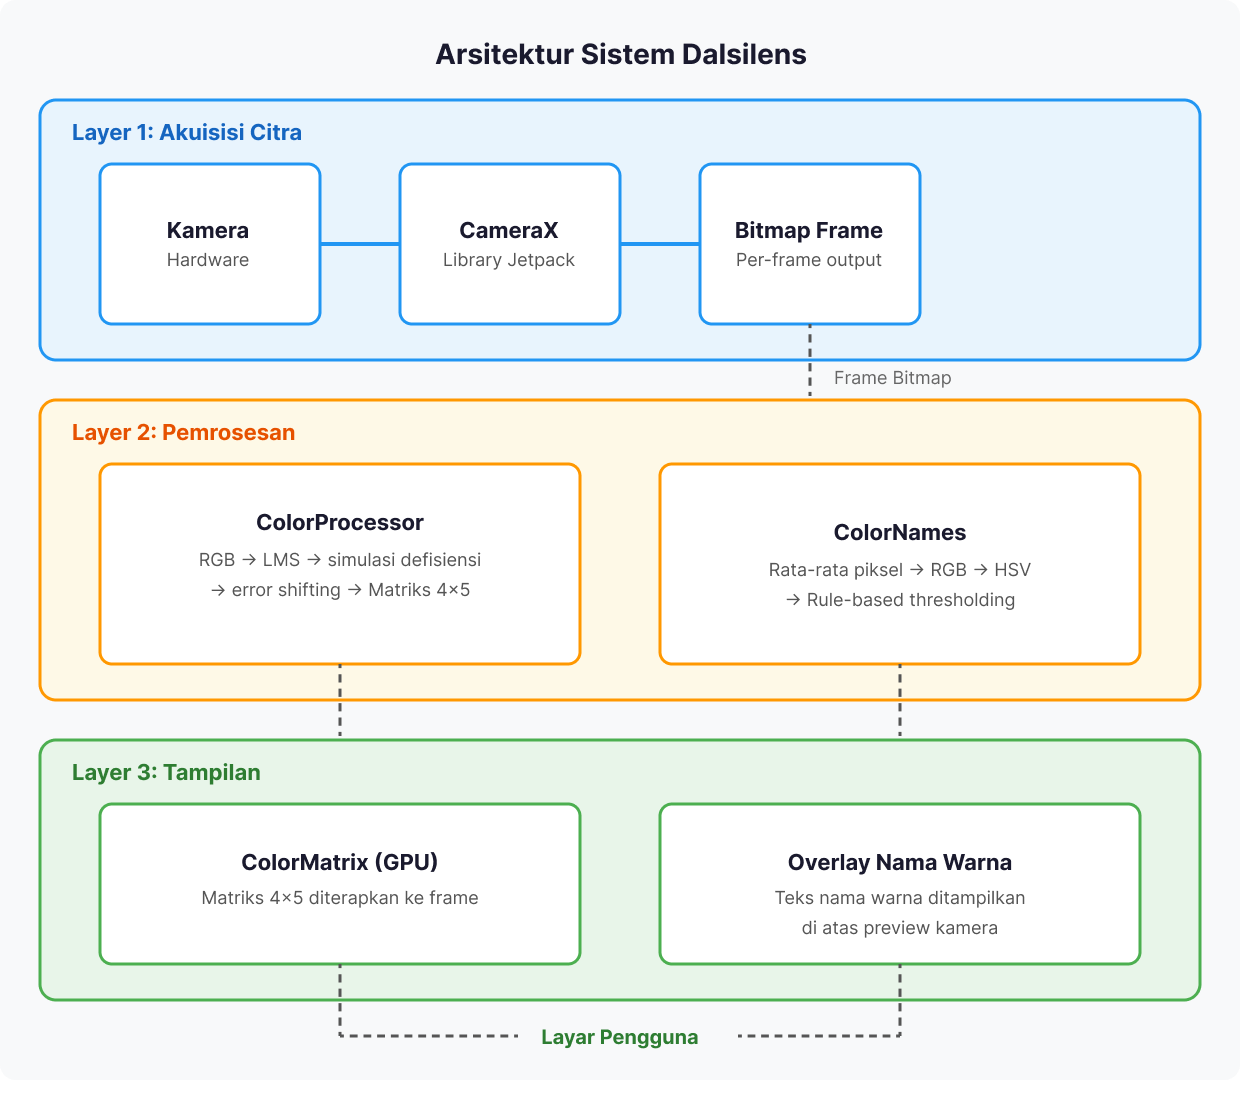
\includegraphics[width=\linewidth]{arsitektur-umum}\\[0.3em]
  {\footnotesize\textit{Figure 1. General Architecture of the Dalsilens System}}
\end{figure}

\subsubsection{Image Acquisition and Color Identification}

The flowchart in Figure 2 describes the early process of processing the image captured by the camera hardware. First, when the user accesses the main interface of the application, the system automatically initializes the camera module. Next, the camera continuously captures each frame and forwards it to the ImageAnalysis component. The image received by this component is then converted into a raw bitmap representation for further processing by system memory. After the conversion process is complete, the system determines a certain Region of Interest (ROI) located exactly in the middle of the bitmap, representing the object that is the target of the crosshair. The system extracts a set of pixels within that ROI for analysis. The extracted pixels are then averaged to obtain a representative RGB value, which is then converted to the HSV color space. The resulting HSV value is then classified using a rule-based thresholding approach to determine the dominant color in the target area. In the final stage, the raw bitmap and the resulting dominant color label are stored in a state variable. Changes to this state then trigger a reactive update of the interface, allowing dynamic visual rendering.

\begin{figure}[H]
  \centering
  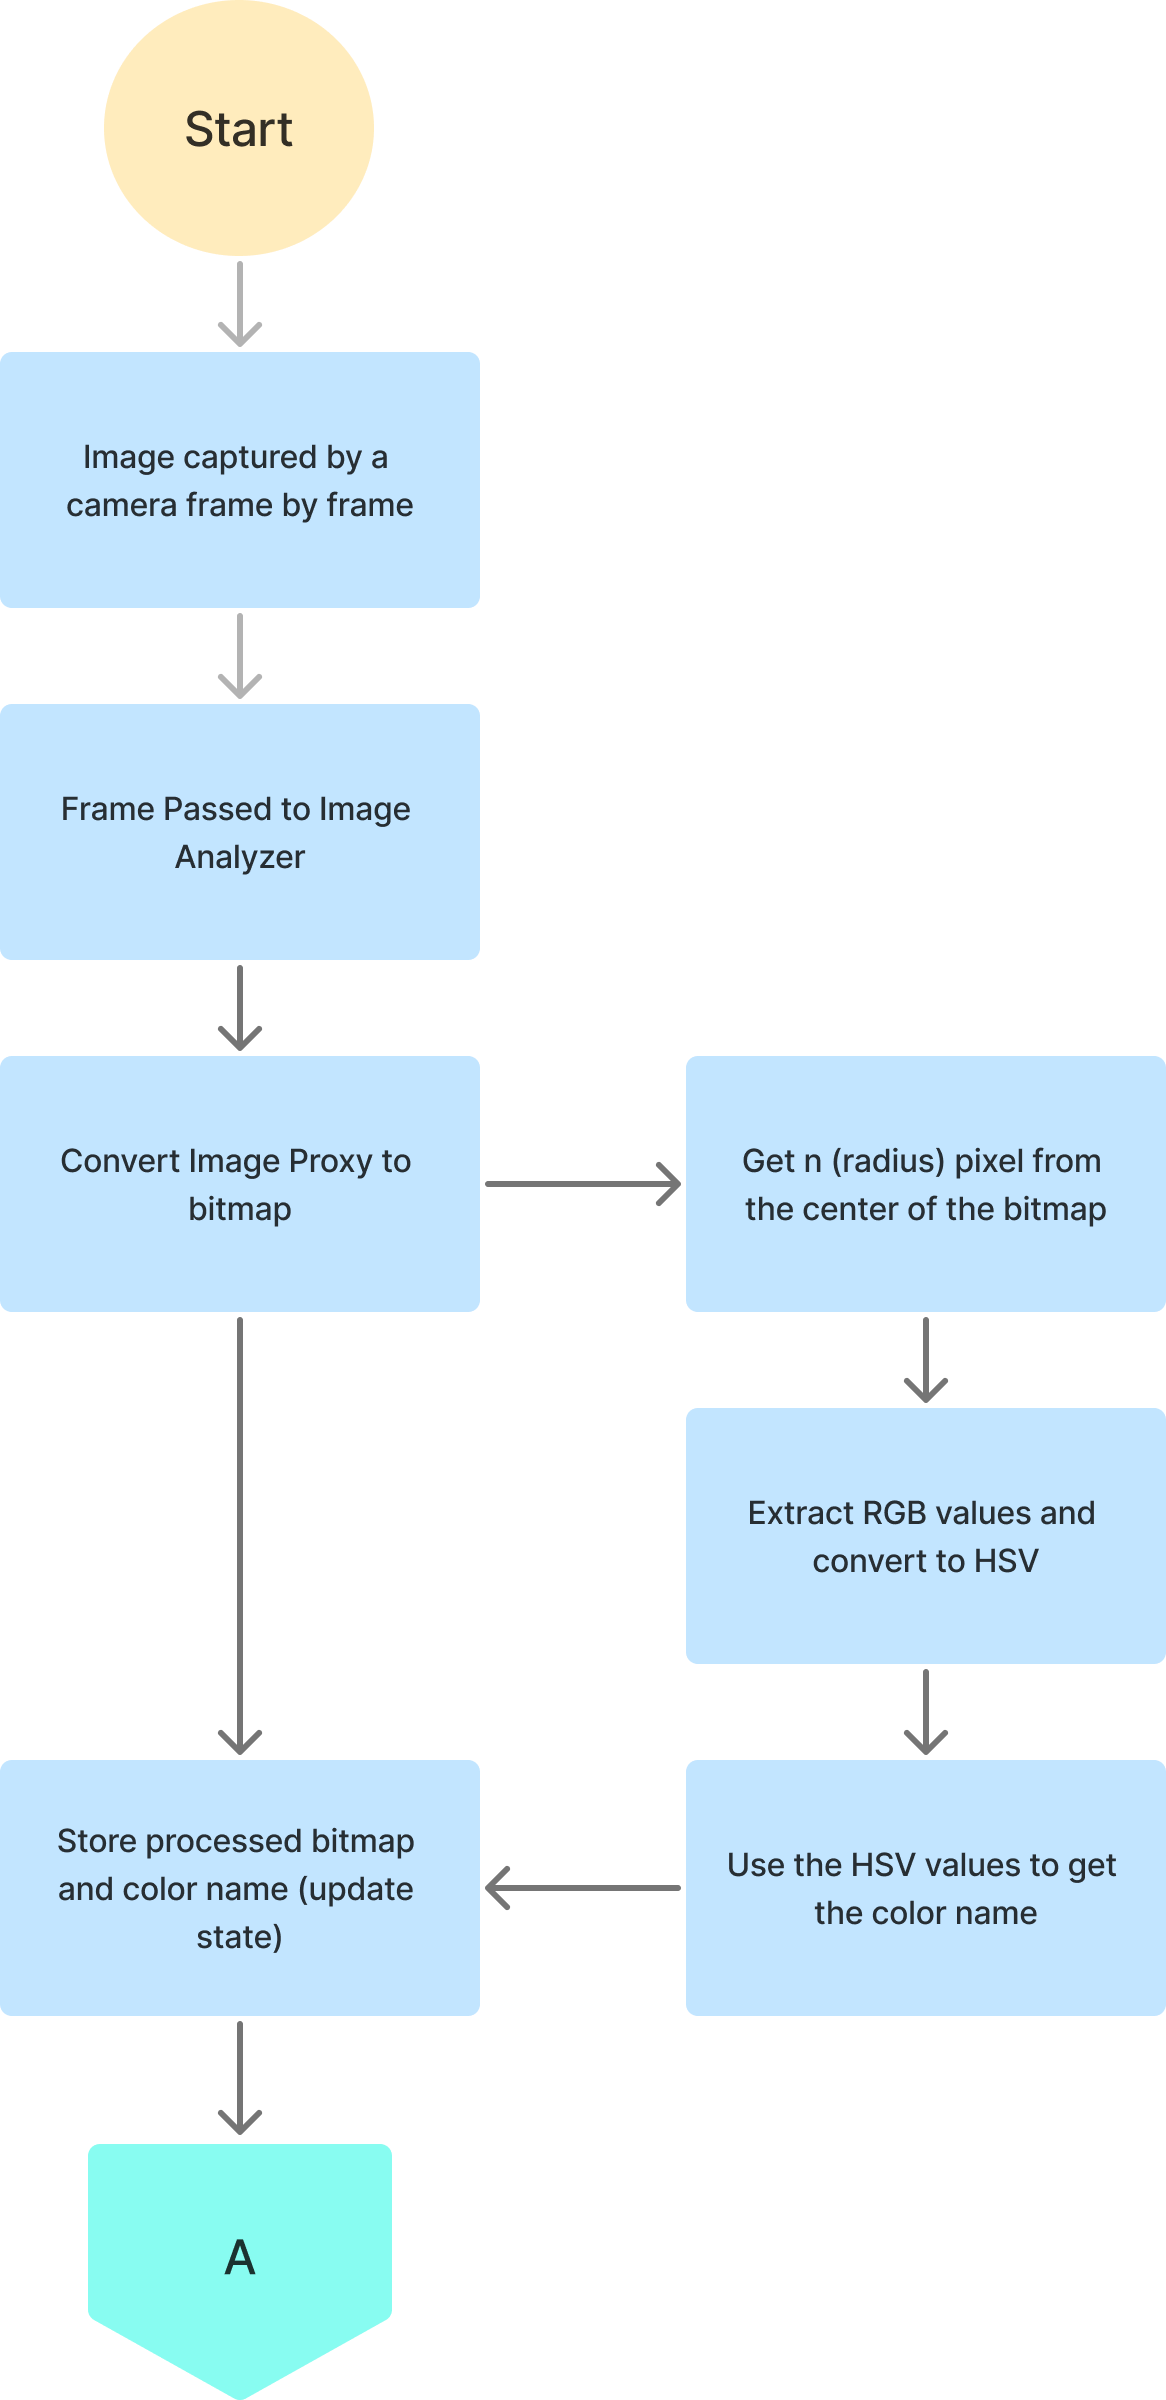
\includegraphics[width=0.8\linewidth]{flowchart-akuisisi}\\[0.3em]
  {\footnotesize\textit{Figure 2. Flowchart of Image Acquisition and Color Identification}}
\end{figure}

\subsubsection{Daltonization Process}

Based on the flowchart in Figure 3, after the bitmap and color label are obtained and stored, the system triggers a reactive update mechanism to update the user interface. Changes to the detected color label are reflected directly on the interface, while the bitmap goes through a verification stage to determine whether the filter has been activated. If the filter is not activated, the system applies an identity color matrix to keep the original color representation of the image. On the other hand, if the filter is activated, the color matrix transformation is applied according to the selected color blindness simulation model. Then, when the daltonization feature is activated, the image is processed further using the LMS-based daltonization algorithm to improve color perception. The bitmap and color matrix that have been determined are then forwarded to the Image component. At this stage, color manipulation is done using a Color Matrix Filter executed through GPU acceleration, so the rendering process can be done efficiently.

\begin{figure}[H]
  \centering
  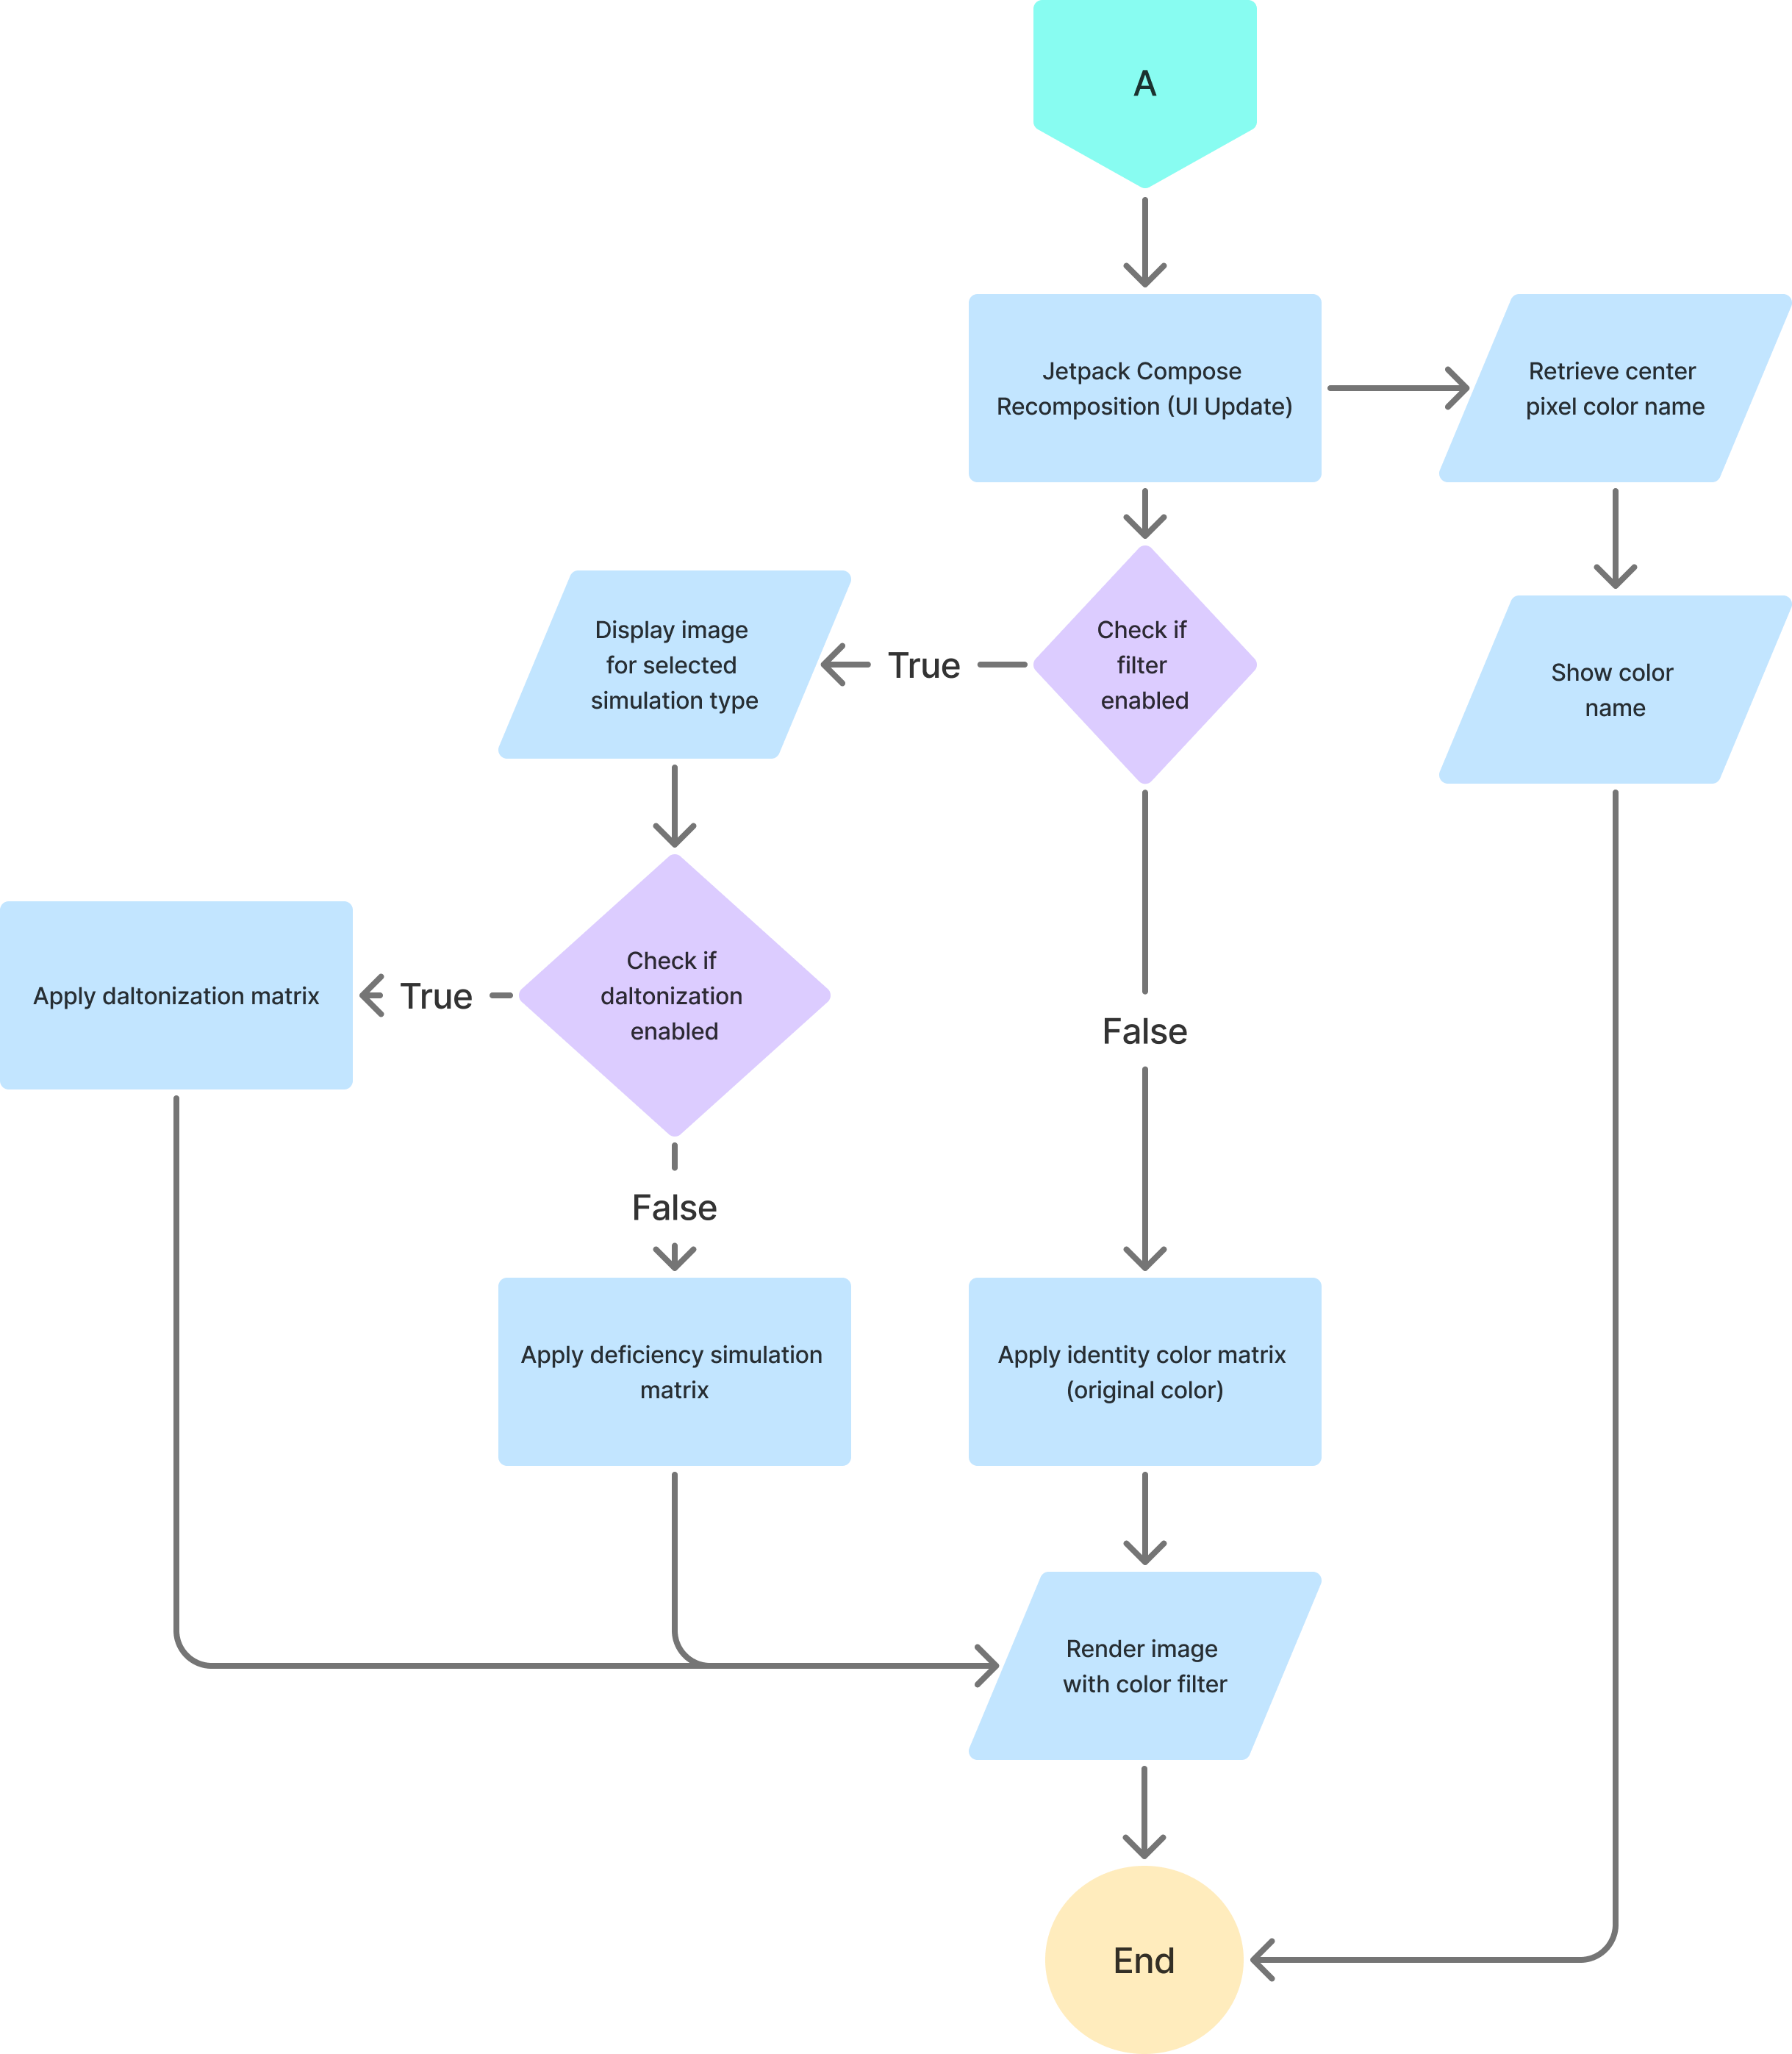
\includegraphics[width=\linewidth]{flowchart-daltonisasi}\\[0.3em]
  {\footnotesize\textit{Figure 3. Flowchart of Color Vision Deficiency Simulation and the Daltonization Process}}
\end{figure}

\subsection{LMS Daltonization Algorithm Implementation}

This section discusses the implementation of the LMS Daltonization algorithm, starting from the RGB-to-LMS conversion, which is the color space the human eye uses to perceive colors, followed by simulation of the color blindness condition, up to the implementation process of the daltonization algorithm.

\subsubsection{RGB to LMS Color Space Conversion}

The first step in implementing this algorithm is converting the image color space from RGB (Red, Green, Blue) to LMS (Long, Medium, Short). This conversion is done using a linear matrix-based transformation, which represents the three types of cone cells in the human visual system. Mathematically, this transformation is done by multiplying the RGB color vector by a certain conversion matrix, so that it produces a color representation in the LMS space. The L, M, and S values in this research are expressed as follows, with the coefficients from [9]:

\begin{equation}
\begin{bmatrix} L \\ M \\ S \end{bmatrix} =
\begin{bmatrix} 17{,}8824 & 43{,}5161 & 4{,}11935 \\ 3{,}4565 & 27{,}1554 & 3{,}86714 \\ 0{,}02996 & 0{,}18431 & 1{,}46709 \end{bmatrix}
\begin{bmatrix} R \\ G \\ B \end{bmatrix}
\end{equation}

The coefficients in this equation are taken from [9], which are used as a reference in the color conversion process from the RGB to the LMS space. These values show the relationship between the RGB elements and the response of each channel in the LMS space, so the conversion result can be applied accurately in the next processing stage. This LMS color space is used as the basis for simulating color vision deficiency and applying the daltonization algorithm in the following stage.

\subsubsection{Color Vision Deficiency Simulation}

The second stage focuses on mathematical modeling to simulate the decrease in color perception ability based on the type of deficiency: Protanopia, Deuteranopia, and Tritanopia. This process is done by modifying the component values in the LMS space obtained from the previous stage. In this condition, one of the components (L, M, or S) loses its sensitivity and is not used directly, but is recalculated based on a combination of the other two components, with transformation coefficients from [10]:

\begin{equation}
\begin{bmatrix} L_{sim} \\ M_{sim} \\ S_{sim} \end{bmatrix}_{Prot} =
\begin{bmatrix} 0 & 2{,}02344 & -2{,}52581 \\ 0 & 1 & 0 \\ 0 & 0 & 1 \end{bmatrix}
\begin{bmatrix} L \\ M \\ S \end{bmatrix}
\end{equation}

\begin{equation}
\begin{bmatrix} L_{sim} \\ M_{sim} \\ S_{sim} \end{bmatrix}_{Deut} =
\begin{bmatrix} 1 & 0 & 0 \\ 0{,}49421 & 0 & 1{,}24827 \\ 0 & 0 & 1 \end{bmatrix}
\begin{bmatrix} L \\ M \\ S \end{bmatrix}
\end{equation}

\begin{equation}
\begin{bmatrix} L_{sim} \\ M_{sim} \\ S_{sim} \end{bmatrix}_{Trit} =
\begin{bmatrix} 1 & 0 & 0 \\ 0 & 1 & 0 \\ -0{,}39591 & 0{,}80111 & 0 \end{bmatrix}
\begin{bmatrix} L \\ M \\ S \end{bmatrix}
\end{equation}

The coefficients in these three equations are taken from [10], [16], which are used to adjust the changes in color components according to the type of deficiency being simulated. In this way, the simulation result can show how colors appear to users with a certain color vision deficiency.

The result of this stage is LMS values that have been modified to simulate the vision condition in color deficiency. These values are then converted back to the RGB space using the inverse matrix of Equation (1), to represent how colors appear to people with color blindness, while also observing the changes in results after applying the daltonization algorithm:

\begin{equation}
\resizebox{0.95\linewidth}{!}{$\displaystyle
\begin{bmatrix} R_{sim} \\ G_{sim} \\ B_{sim} \end{bmatrix} =
\begin{bmatrix} 0{,}08094 & -0{,}13050 & 0{,}11672 \\ -0{,}01025 & 0{,}05402 & -0{,}11362 \\ -0{,}00037 & -0{,}00412 & 0{,}69351 \end{bmatrix}
\begin{bmatrix} L_{sim} \\ M_{sim} \\ S_{sim} \end{bmatrix}$}
\end{equation}

\subsubsection{Daltonization Process}

At this stage, the daltonization process is done by calculating the difference between the original color and the color from the color deficiency simulation. The calculation starts by converting the color value from the RGB to the LMS space, simulating the color deficiency in the LMS space, then converting it back to the RGB space. The difference between the original color and the simulated color is then calculated as the error value:

\begin{equation}
E_R = R - R_{sim}, \quad E_G = G - G_{sim}, \quad E_B = B - B_{sim}
\end{equation}

After the error value is obtained, the next step is redistributing the value to other color components through an error shifting process. This process is done because the color components affected by the deficiency cannot be perceived optimally by the user, so the missing color information needs to be moved to other color components that can still be told apart. This redistribution is done using a different transformation matrix for each type of deficiency, in order to adjust the direction of the error distribution to the color components that can still be perceived optimally.

In the Protanopia condition, the red component has reduced sensitivity so it does not receive error distribution, and all of the error is moved to the green and blue components. In Deuteranopia, the green component is the most affected so it is not used in redistribution, and the error is moved to the red and blue components. Meanwhile, in Tritanopia, the blue component has reduced sensitivity, so the error is moved to the red and green components. The coefficients of the following three matrices are taken from [8], [10], [16]:

\begin{equation}
\begin{bmatrix} R_{shift} \\ G_{shift} \\ B_{shift} \end{bmatrix}_{Prot} =
\begin{bmatrix} 0 & 0 & 0 \\ 0{,}7 & 1 & 0 \\ 0{,}7 & 0 & 1 \end{bmatrix}
\begin{bmatrix} E_R \\ E_G \\ E_B \end{bmatrix}
\end{equation}

\begin{equation}
\begin{bmatrix} R_{shift} \\ G_{shift} \\ B_{shift} \end{bmatrix}_{Deut} =
\begin{bmatrix} 1 & 0{,}7 & 0 \\ 0 & 0 & 0 \\ 0 & 0{,}7 & 1 \end{bmatrix}
\begin{bmatrix} E_R \\ E_G \\ E_B \end{bmatrix}
\end{equation}

\begin{equation}
\begin{bmatrix} R_{shift} \\ G_{shift} \\ B_{shift} \end{bmatrix}_{Trit} =
\begin{bmatrix} 1 & 0 & 0{,}7 \\ 0 & 1 & 0{,}7 \\ 0 & 0 & 0 \end{bmatrix}
\begin{bmatrix} E_R \\ E_G \\ E_B \end{bmatrix}
\end{equation}

The shifted error value is then added back to the original color to produce the corrected (daltonized) color:

\begin{equation}
R_{d} = R + R_{shift}, \; G_{d} = G + G_{shift}, \; B_{d} = B + B_{shift}
\end{equation}

\subsubsection{Construction of the 4$\times$5 Transformation Matrix}

At this stage, all of the color transformation processes described previously are represented as a transformation function $T(R,G,B)$. To optimize the computing load and avoid repeated pixel calculation, this transformation function is simplified into a constant matrix of size 4$\times$5. The simplification is done by evaluating the function $T$ against three primary color vectors: pure red $(1,0,0)$, pure green $(0,1,0)$, and pure blue $(0,0,1)$:

\begin{equation}
\begin{aligned}
T(1,0,0) &= (r_R, r_G, r_B) \\
T(0,1,0) &= (g_R, g_G, g_B) \\
T(0,0,1) &= (b_R, b_G, b_B)
\end{aligned}
\end{equation}

The transformation results of these three basis vectors are then arranged into the coefficient columns of the matrix $M_{dalton}$, so that this matrix can directly map the original color profile into the corrected color, while also keeping the alpha (transparency) parameter on the fourth row:

\begin{equation}
M_{dalton} =
\begin{bmatrix}
r_R & g_R & b_R & 0 & 0 \\
r_G & g_G & b_G & 0 & 0 \\
r_B & g_B & b_B & 0 & 0 \\
0 & 0 & 0 & 1 & 0
\end{bmatrix}
\end{equation}

This $M_{dalton}$ matrix is the one directly applied to the Android ColorMatrix and executed through GPU acceleration, so there is no need to recalculate Equations (1) to (10) for each image pixel in real-time.

\subsection{Severity Level Implementation}

This section explains how the adjustment of the color deficiency severity level is implemented dynamically. The severity parameter is represented in the decimal range 0.0 to 1.0. To keep the accuracy of the visual representation, the system distinguishes the method of applying severity based on its purpose, namely between the vision simulation process and the daltonization process.

\subsubsection{Severity Modeling in the Deficiency Simulation}

In simulation mode, the severity parameter works to imitate the level of damage or shift in sensitivity of the user's cone cells. This process approaches a medical condition known as Anomalous Trichromacy [11]. Therefore, the calculation is done directly in the LMS color space using a linear interpolation method. The system calculates the difference between the LMS value in normal vision conditions and the LMS value in full deficiency conditions, then multiplies this difference by the severity parameter and adds it back to the normal value:

\begin{equation}
L_{f} = L_{n} + (L_{sim} - L_{n}) \times S
\end{equation}

\subsubsection{Severity Modeling in Color Vision Correction}

Different from the simulation stage, the severity parameter in the daltonization process works to determine the intensity or strength of the color aid given to the user. This calculation is done in the RGB color space, specifically at the final computing stage when the shifted error value is added to the original pixel. The compensation intensity is adjusted by multiplying the shifted error result of each color channel by the severity value, before it is combined with the original color, so the user can adjust the color contrast proportionally according to their visual comfort:

\begin{equation}
R_{d} = R + (R_{shift} \times S)
\end{equation}

\subsection{Dominant Color Extraction Based on the HSV Color Space}

This section discusses the process of extracting the dominant color based on the HSV color space. This stage aims to extract the color of the object at the center point that is the target of the crosshair in real-time. This process starts by obtaining the image in bitmap form, continues with processing the pixel area around the center point, and ends with classifying the color name using the HSV color space.

\subsubsection{Bitmap Acquisition and Processing}

The frame from the camera is obtained through the ImageAnalysis component in CameraX, which continuously captures images. The frame is then forwarded to the analyzer function, which produces an ImageProxy, before it is finally converted into a Bitmap. Because the camera sensor orientation varies between Android devices, the rotationDegrees value in the frame metadata is checked. If the rotation value is not zero, the bitmap is rotated using a transformation matrix.

\subsubsection{Pixel Sampling}

Color sampling is not only done on one pixel at the center of the screen, because a single pixel sample tends to be less effective since the color of an area can be affected by noise, lighting, or other conditions. Therefore, a sampling approach is used by taking several pixels around the center point, so the resulting color becomes more stable and can represent the dominant color in the observed area better.

The first step is determining the sampling area radius, with a default radius value of $r=5$. With this radius, the sample area taken covers 121 pixels (11 x 11). The number of pixels used can be calculated using the following equation:

\begin{equation}
N = (2r+1) \times (2r+1)
\end{equation}

Given an image $I$ of size $W \times H$ and a center point $(x_c, y_c)$ with radius $r$, a bounding function is defined so that the processed pixel coordinates do not exceed the image boundaries:

\begin{equation}
f(x) = \min(\max(x, 0), W-1)
\end{equation}
\begin{equation}
g(y) = \min(\max(y, 0), H-1)
\end{equation}

Each pixel at coordinates $(x,y)$ is stored as a 32-bit integer in ARGB format. The bit structure of the blue component (B) is at the very last position, so no bit shift is needed, only masking to remove the other bits using a mask value of 255 (0xFF). Meanwhile, the green component (G) is in the middle position so it needs to be shifted to the right by eight bits first, and the red component (R) is at the very left position so it needs to be shifted to the right by 16 bits. The three color components are extracted through bit shift and masking operations against the pixel value:

\begin{equation}
B_{(x,y)} = \text{pixel} \mathbin{\&} 255
\end{equation}
\begin{equation}
G_{(x,y)} = (\text{pixel} \gg 8) \mathbin{\&} 255
\end{equation}
\begin{equation}
R_{(x,y)} = (\text{pixel} \gg 16) \mathbin{\&} 255
\end{equation}

The average RGB value of all $N$ pixels in the sample area is then calculated as the representation of the dominant color:

\begin{equation}
\bar{R} = \frac{1}{N}\sum_{i=1}^{N} R_i, \quad
\bar{G} = \frac{1}{N}\sum_{i=1}^{N} G_i, \quad
\bar{B} = \frac{1}{N}\sum_{i=1}^{N} B_i
\end{equation}

\subsubsection{Color Name Classification}

The final stage is color classification, which is done by converting the obtained average RGB value to the HSV color space using the built-in Android function in the android.graphics.Color class, namely RGBToHSV(r, g, b, hsv). The conversion result consists of three components: Hue (H) as the type of color in the range $0^\circ$--$360^\circ$, Saturation (S) as the intensity level of the color in the range 0 to 1, and Value (V) as the brightness level in the range 0 to 1. These three components are then used to determine the color name using a threshold approach based on the range of H, S, and V values. The threshold values are determined by testing color samples under normal and dim lighting conditions, by considering the average, standard deviation, and tolerance range.

As an example, the following calculation determines the range of H values for the color red. The test data is obtained from 10 samples under normal lighting and 10 samples under dim lighting, which is then used to calculate the average value and the variation range of the Hue component. The calculation results show that the average Hue value under normal lighting is $3.3^\circ$, while under dim lighting it is $8.1^\circ$. Then, the standard deviation is calculated to find the data spread in each condition, and a standard deviation of $0.48^\circ$ is obtained in normal conditions and $0.88^\circ$ in dim conditions.

The tolerance value (upper and lower limits) is then determined by adding and subtracting the average with the standard deviation, using the equation $\bar{H} \pm 2\sigma$. The lower limit for normal lighting is obtained from $3.3 - 2(0.48^\circ) = 2.34^\circ$, while the upper limit is obtained from $3.3 + 2(0.48^\circ) = 4.26^\circ$, so the tolerance range in normal conditions is between $2.34^\circ$ and $4.26^\circ$. The same method is applied in dim conditions, with the lower limit $8.1 - 2(0.88^\circ) = 6.34^\circ$ and the upper limit $8.1 + 2(0.88^\circ) = 9.86^\circ$, so the tolerance range in dim conditions is between $6.34^\circ$ and $9.86^\circ$.

When compared, the Hue value ranges of normal and dim conditions do not overlap. Based on this result, the threshold value is determined by setting the upper limit of the condition with the largest variation, which is $9.86^\circ$, so the threshold value for the color red is stated as H $< 9.86^\circ$. The same method is applied to the other colors, producing a threshold table that can be used directly in the color classification process, as shown in Table 1.

\begin{table}[H]
  \centering
  {\footnotesize
  \begin{tabular}{|c|c|}
    \hline
    \textbf{Hue Range ($^\circ$)} & \textbf{Color Category} \\
    \hline
    H $<$ 9.85 & Red \\ \hline
    9.85 $\leq$ H $<$ 26.98 & Orange \\ \hline
    26.98 $\leq$ H $<$ 50.42 & Yellow \\ \hline
    50.42 $\leq$ H $<$ 122.50 & Green \\ \hline
    122.50 $\leq$ H $<$ 204.85 & Cyan \\ \hline
    204.85 $\leq$ H $<$ 224.57 & Blue \\ \hline
    224.57 $\leq$ H $<$ 319.37 & Purple \\ \hline
    H $\geq$ 319.37 & Red \\ \hline
  \end{tabular}}\\[0.3em]
  {\footnotesize\textit{Table 1. Color Classification Based on the Hue Range}}
\end{table}

Colors with a low Saturation value are not classified using Hue because they tend to be achromatic (grayscale), so their classification instead uses the Value to tell apart the categories Black, Dark Gray, Gray, and White, as shown in Table 2.

\begin{table}[H]
  \centering
  {\footnotesize
  \begin{tabular}{|c|c|c|}
    \hline
    \textbf{Saturation} & \textbf{Value} & \textbf{Category} \\
    \hline
    S $<$ 0.10 & V $<$ 0.15 & Black \\ \hline
    S $<$ 0.10 & 0.15 $\leq$ V $<$ 0.40 & Dark Gray \\ \hline
    S $<$ 0.10 & 0.40 $\leq$ V $<$ 0.78 & Gray \\ \hline
    S $<$ 0.10 & V $\geq$ 0.78 & White \\ \hline
  \end{tabular}}\\[0.3em]
  {\footnotesize\textit{Table 2. Achromatic Color Classification Based on Saturation and Value}}
\end{table}

By combining the classification based on Hue, Saturation, and Value, the system can recognize both chromatic and achromatic colors in real-time, even when the surrounding lighting conditions vary.

\subsection{Test Scenarios}

Application testing covers four scenarios: (1) functionality testing using Black Box Testing [12] against 15 usage scenarios; (2) color name classification accuracy testing against 10 color categories under normal and dim lighting conditions; (3) real-time performance testing in the form of FPS, latency, RAM usage, and CPU utilization using adb shell dumpsys and the Android Studio Profiler; and (4) usability testing using the System Usability Scale (SUS) questionnaire [13] against 18 respondents, consisting of both people with color vision deficiency and people with normal color vision.

% ============================================================
% 4. RESULTS AND DISCUSSION
% ============================================================
\section{Results and Discussion}

\subsection{Functionality Testing}

Black Box Testing [12] was carried out against 15 scenarios covering interface navigation, filter activation/deactivation, selection of the simulation type (Protanopia, Deuteranopia, Tritanopia), severity setting, sampling area size setting, and real-time color name detection. Each scenario was tested by giving certain input and verifying that the output matches the designed expectation, starting from interface navigation, filter activation and deactivation, selection of the three types of color blindness simulation, severity setting at minimum and maximum values, up to the sampling area size setting. All 15 scenarios produced \textbf{Successful} output, showing that the main features of the application run according to the design expectation without any functional failure found.

\subsection{Color Classification Accuracy Testing}

The testing was carried out against 10 physical objects representing each color category, under two lighting conditions: \textbf{normal} (standard room lighting) and \textbf{dim} (light reduced using curtains). The detected color name was compared with the actual color of the object, as shown in Table 3 and Table 4.

\begin{table}[H]
  \centering
  {\scriptsize
  \begin{tabular}{|c|l|l|l|c|}
    \hline
    \textbf{No.} & \textbf{Object} & \textbf{Actual} & \textbf{Detected} & \textbf{Result} \\
    \hline
    1 & Rope & Red & Red & Correct \\ \hline
    2 & Shirt & Orange & Orange & Correct \\ \hline
    3 & Shirt & Yellow & Yellow & Correct \\ \hline
    4 & Teapot & Green & Green & Correct \\ \hline
    5 & Keyboard cleaner & Cyan & Cyan & Correct \\ \hline
    6 & Keychain & Blue & Blue & Correct \\ \hline
    7 & Student ID card & Purple & Magenta & Wrong \\ \hline
    8 & Tumbler & White & White & Correct \\ \hline
    9 & Pants & Black & Black & Correct \\ \hline
    10 & Clothesline hook & Gray & Gray & Correct \\ \hline
  \end{tabular}}\\[0.3em]
  {\footnotesize\textit{Table 3. Color Classification Test Results Under Normal Lighting}}
\end{table}

\begin{table}[H]
  \centering
  {\scriptsize
  \begin{tabular}{|c|l|l|l|c|}
    \hline
    \textbf{No.} & \textbf{Object} & \textbf{Actual} & \textbf{Detected} & \textbf{Result} \\
    \hline
    1 & Rope & Red & Red & Correct \\ \hline
    2 & Shirt & Orange & Orange & Correct \\ \hline
    3 & Shirt & Yellow & Orange & Wrong \\ \hline
    4 & Teapot & Green & Green & Correct \\ \hline
    5 & Keyboard cleaner & Cyan & Blue & Wrong \\ \hline
    6 & Keychain & Blue & Blue & Correct \\ \hline
    7 & Student ID card & Purple & Red & Wrong \\ \hline
    8 & Tumbler & White & Gray & Wrong \\ \hline
    9 & Pants & Black & Black & Correct \\ \hline
    10 & Clothesline hook & Gray & Yellow & Wrong \\ \hline
  \end{tabular}}\\[0.3em]
  {\footnotesize\textit{Table 4. Color Classification Test Results Under Dim Lighting}}
\end{table}

Based on Table 3 and Table 4, the detection accuracy under normal lighting conditions is $\frac{9}{10} \times 100\% = 90\%$, with one error on the color purple being detected as magenta. Under dim lighting conditions, accuracy drops to $\frac{5}{10} \times 100\% = 50\%$, as summarized in Table 5.

\begin{table}[H]
  \centering
  {\footnotesize
  \begin{tabular}{|l|c|c|}
    \hline
    \textbf{Lighting Condition} & \textbf{Correct} & \textbf{Accuracy} \\
    \hline
    Normal & 9/10 & 90\% \\ \hline
    Dim & 5/10 & 50\% \\ \hline
  \end{tabular}}\\[0.3em]
  {\footnotesize\textit{Table 5. Summary of Color Name Classification Accuracy}}
\end{table}

The drop in accuracy in dim conditions happens because the Value (V) in the HSV color space decreases significantly, so pixels that should be classified as colored tend to be detected as gray or black. This finding is consistent with research [14] which states that smartphone-based colorimetric accuracy in the HSV color space is sensitive to lighting conditions.

\subsection{Real-Time Performance Testing}

Performance testing was carried out in the highest computing load scenario, namely when the daltonization mode and color identification run together, representing the worst-case condition that may occur. FPS and latency testing was done using frame rendering statistics data from the adb shell dumpsys gfxinfo command, in three iterations, each running for roughly one minute, as shown in Table 6.

\begin{table}[H]
  \centering
  {\footnotesize
  \begin{tabular}{|l|c|c|c|c|}
    \hline
    \textbf{Iteration} & \textbf{Frame} & \textbf{FPS} & \textbf{Latency (ms)} & \textbf{Janky (\%)} \\
    \hline
    1 & 2,389 & 55.0 & 18.2 & 28.59 \\ \hline
    2 & 2,808 & 65.3 & 15.3 & 9.62 \\ \hline
    3 & 1,134 & 46.8 & 21.4 & 23.10 \\ \hline
    \textbf{Average} & \textbf{6,331} & \textbf{57.2} & \textbf{17.5} & \textbf{19.19} \\ \hline
  \end{tabular}}\\[0.3em]
  {\footnotesize\textit{Table 6. FPS and Processing Latency Test Results}}
\end{table}

The average value of 57.2 FPS with a latency of 17.5 ms shows that the application is close to a smooth real-time condition (60 FPS) even though the color matrix transformation and color classification run together. The GPU Rendering Profile data shows that the median GPU processing time is in the 5--7 ms range, far lower than the total render time per frame, indicating that color transformation is not the main bottleneck.

Memory usage was measured through the Total Proportional Set Size (PSS) using the adb shell dumpsys meminfo command, as shown in Table 7.

\begin{table}[H]
  \centering
  {\footnotesize
  \begin{tabular}{|l|c|c|}
    \hline
    \textbf{Iteration} & \textbf{PSS (KB)} & \textbf{PSS (MB)} \\
    \hline
    1 & 223,147 & 217.92 \\ \hline
    2 & 227,867 & 222.53 \\ \hline
    3 & 220,339 & 215.18 \\ \hline
    \textbf{Average} & \textbf{223,784} & \textbf{218.54} \\ \hline
  \end{tabular}}\\[0.3em]
  {\footnotesize\textit{Table 7. Memory (RAM) Usage Test Results}}
\end{table}

The PSS values in the three test iterations are within a narrow range ($\pm$3.5 MB from the average) without showing a consistent upward trend between iterations, so no signs of a memory leak were found in the Dalsilens application.

CPU utilization was measured using the adb shell top -n 2 -d 1 command, with the recorded value being the second sample of each measurement pair, as shown in Table 8.

\begin{table}[H]
  \centering
  {\footnotesize
  \begin{tabular}{|l|c|}
    \hline
    \textbf{Iteration} & \textbf{CPU Utilization (\%)} \\
    \hline
    1 & 147 \\ \hline
    2 & 148 \\ \hline
    3 & 166 \\ \hline
    \textbf{Average} & \textbf{153.67} \\ \hline
  \end{tabular}}\\[0.3em]
  {\footnotesize\textit{Table 8. CPU Utilization Test Results}}
\end{table}

The CPU utilization value exceeds 100\% because Linux/Android-based utilities such as top calculate the CPU percentage as the accumulated usage across all cores used by the process, not relative to a single core. The test device has a total CPU capacity of 800\% (8 cores), so the average value of 153.67\% when converted into a percentage relative to the total device capacity produces:

\begin{equation}
\text{Relative CPU Utilization} = \frac{153{,}67\%}{8 \times 100\%} \times 100\% \approx 19{,}21\%
\end{equation}

This value shows that the Dalsilens application only uses around 19.21\% of the total CPU computing capacity of the device even while running the color matrix transformation and color classification at the same time, proving the effectiveness of moving the heavy computing load from the CPU to the GPU through the ColorMatrix [8].

\noindent
\begin{minipage}[t]{0.48\linewidth}
  \centering
  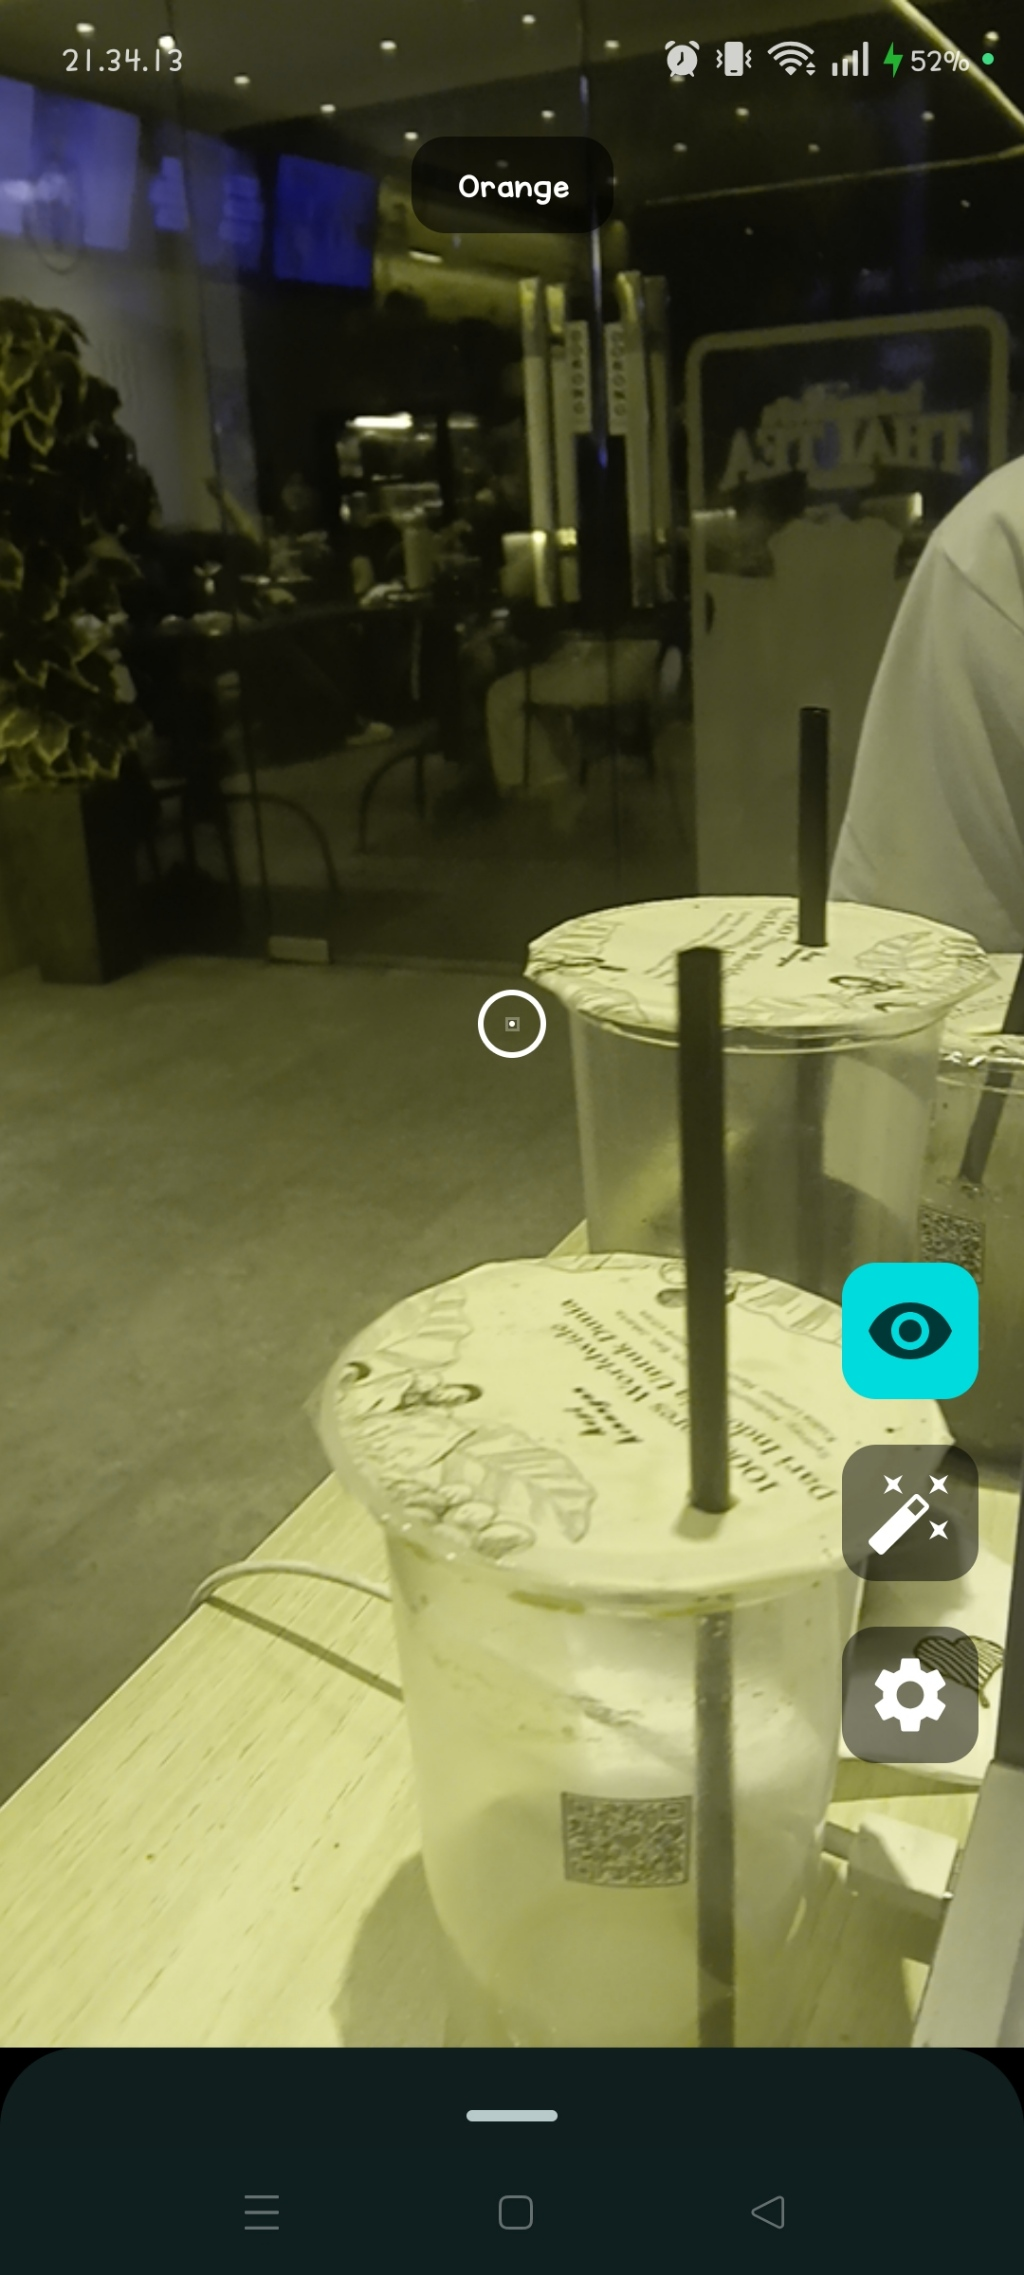
\includegraphics[width=\linewidth]{ss_deuteranopia}\\[0.2em]
  {\footnotesize\textit{Deuteranopia Simulation}}
\end{minipage}
\hfill
\begin{minipage}[t]{0.48\linewidth}
  \centering
  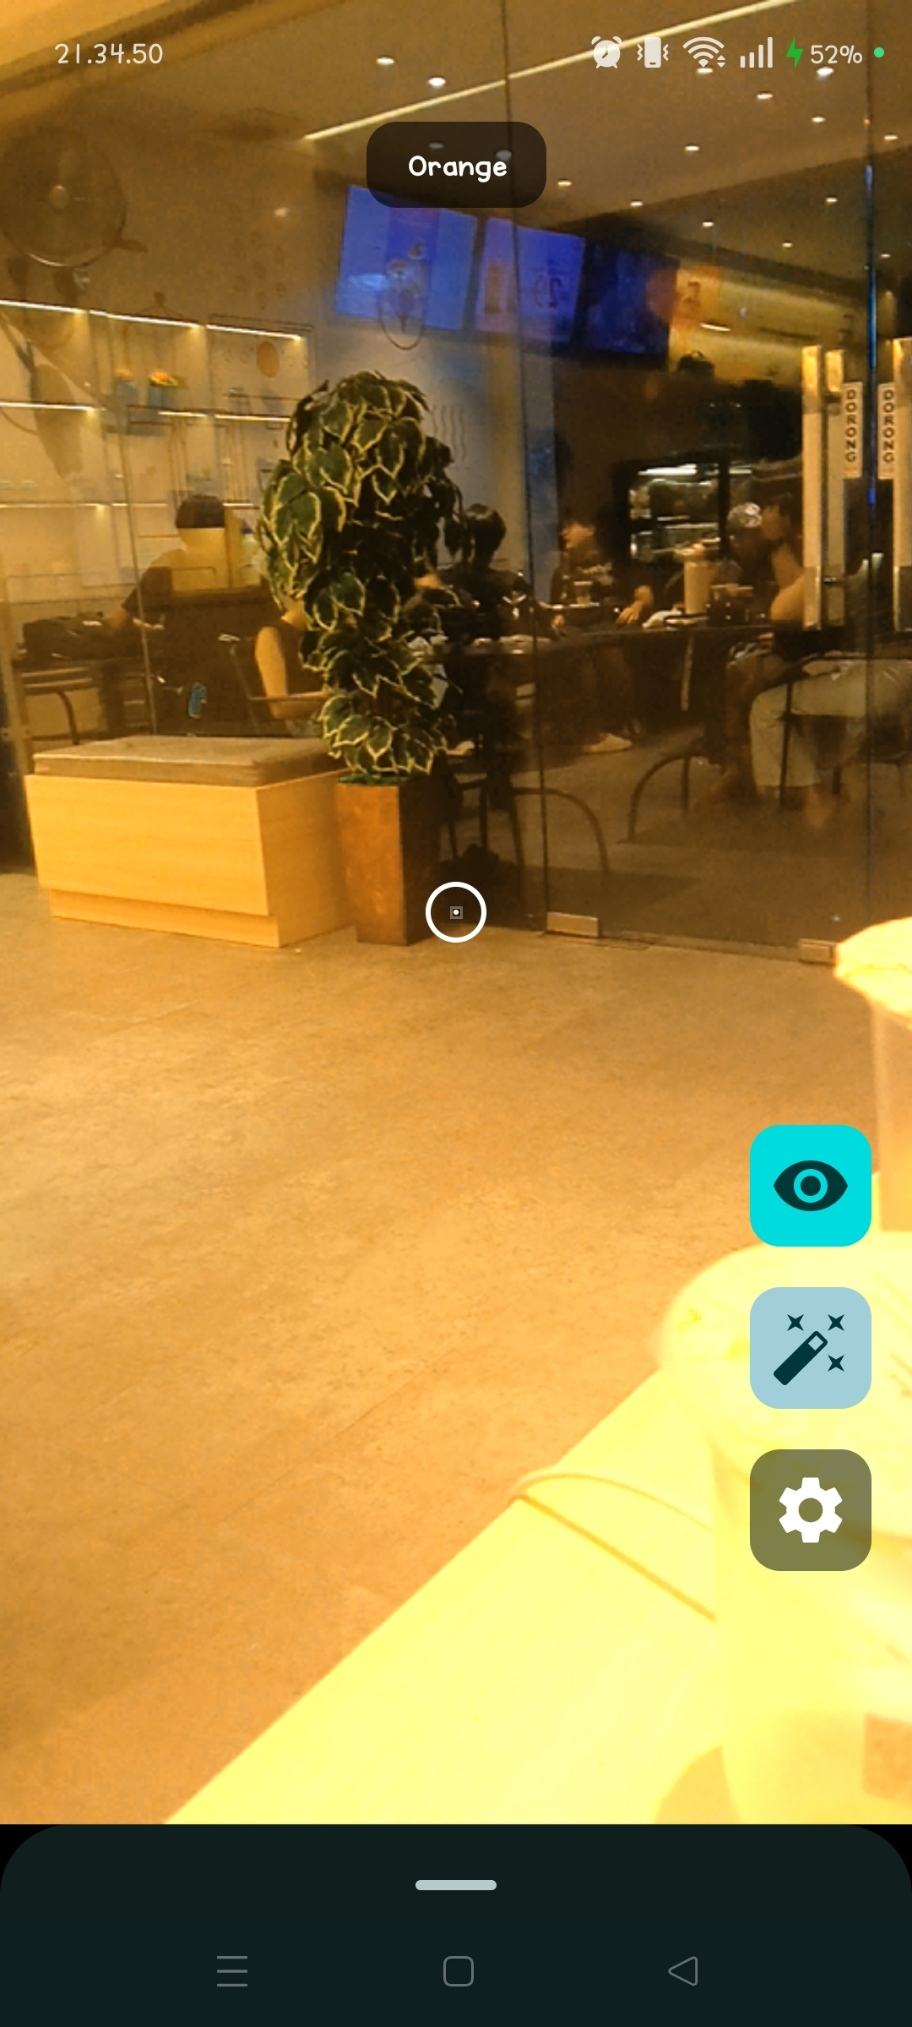
\includegraphics[width=\linewidth]{ss_daltonization}\\[0.2em]
  {\footnotesize\textit{Simulation + Daltonization}}
\end{minipage}
\vspace{0.3em}

\begin{center}
  {\footnotesize\textit{Figure 4. Comparison of the Deuteranopia Simulation View Before and After Daltonization}}
\end{center}

As shown in Figure 4, applying daltonization shifts the object colors to different hues from the pure simulation result, helping people with Deuteranopia tell apart objects that previously looked similar.

\subsection{Usability Testing (SUS)}

The System Usability Scale (SUS) is a standard questionnaire developed by Brooke [13] to measure the level of usability of a system quickly and efficiently, consisting of 10 statements with a Likert scale of 1 to 5, where odd-numbered statements are positive and even-numbered statements are negative [15]. The SUS score is calculated using the following equation [13]:

\begin{equation}
\text{SUS Score} = \left(\sum_{i \in \text{odd}}(x_i - 1) + \sum_{j \in \text{even}}(5 - x_j)\right) \times 2{,}5
\end{equation}

where $x_i$ is the respondent's answer value for statement $i$, and the resulting score is in the range of 0 to 100. The interpretation of the SUS score refers to the classification in Table 9.

\begin{table}[H]
  \centering
  {\footnotesize
  \begin{tabular}{|c|c|c|}
    \hline
    \textbf{Score Range} & \textbf{Grade} & \textbf{Category} \\
    \hline
    $>$ 80.3 & A & \textit{Excellent} \\ \hline
    68 -- 80.3 & B & \textit{Good} \\ \hline
    57 -- 68 & C & \textit{OK} \\ \hline
    $<$ 57 & D & \textit{Poor} \\ \hline
  \end{tabular}}\\[0.3em]
  {\footnotesize\textit{Table 9. System Usability Scale Score Classification}}
\end{table}

The testing was carried out against 18 respondents who tried the Dalsilens application directly on their respective Android devices for about five minutes, then filled out the SUS questionnaire. The respondents were not all affected by CVD: the group included both people with color vision deficiency and people with normal color vision, so that the usability of the application could be assessed from both perspectives. The demographic data of the respondents (anonymized as R1--R18) is presented in Table 10.

\begin{table}[H]
  \centering
  {\footnotesize
  \begin{tabular}{|c|c|c||c|c|c|}
    \hline
    \textbf{Resp.} & \textbf{Age} & \textbf{G} & \textbf{Resp.} & \textbf{Age} & \textbf{G} \\\hline
    R1  & 20 & M & R10 & 20 & F \\ \hline
    R2  & 31 & M & R11 & 20 & M \\ \hline
    R3  & 21 & M & R12 & 19 & M \\ \hline
    R4  & 20 & F & R13 & 19 & F \\ \hline
    R5  & 21 & F & R14 & 21 & M \\ \hline
    R6  & 21 & M & R15 & 15 & M \\ \hline
    R7  & 28 & M & R16 & 20 & F \\ \hline
    R8  & 22 & M & R17 & 21 & M \\ \hline
    R9  & 20 & F & R18 & 20 & M \\ \hline
  \end{tabular}}\\[0.3em]
  {\footnotesize\textit{Table 10. Demographic Data of SUS Testing Respondents (G: Gender, M: Male, F: Female)}}
\end{table}

The recap of all respondents' answers to the 10 SUS statements (P1--P10) produces SUS scores that vary between 47.5 and 90.0, with an average score of 68.33. This average value falls into category B (Good) according to Table 9. This result shows that the Dalsilens application is rated well and is acceptable to users in terms of ease and comfort of use, although there is still room for improvement in the interface aspect to reach the Excellent category.

Overall, the test results show that the GPU-accelerated ColorMatrix-based approach successfully answers the performance challenge faced by the manual calculation approach in previous research [6], while the direct integration into a real-time camera overcomes the static processing limitation in [5]. The high precision level in most color categories (Table 3) indicates a minimal false positive error rate in the color identification context, while the decreasing color classification accuracy in dim conditions (Table 4) is the main limitation that needs attention in further development, for example through a machine learning-based approach that is more adaptive to lighting variations. The gap between academic research and practical application is also bridged through an intuitive interface, so users can get instant visual and textual feedback without needing additional processing outside the device.

% ============================================================
% 5. CONCLUSION
% ============================================================
\section{Conclusion}

The Dalsilens application was successfully developed as an Android-based real-time visual aid for people with dichromacy, integrating the LMS Daltonization algorithm and the HSV-based color name identification feature. All 15 Black Box Testing scenarios ran \textbf{Successfully}, color classification accuracy reached 90\% under normal lighting but dropped under dim lighting, real-time performance averaged 57.2 FPS with a latency of 17.5 ms without signs of memory leaks, and the relative CPU utilization was only 19.21\% thanks to moving the computing load to the GPU through the ColorMatrix. The SUS score of 68.33 (Category B/Good) shows a good level of usability. Further research is suggested to apply a machine learning-based approach to improve color classification accuracy under varied lighting conditions, and to expand support to the Anomalous Trichromacy type.

% ============================================================
% REFERENCES
% ============================================================
\section*{\fontsize{11}{13}\selectfont\bfseries REFERENCES}

{\footnotesize
\begin{enumerate}[leftmargin=1.4em, itemsep=0.3em, label={[\arabic*]}]
  \item D. Man and R. Olchawa, `The Possibilities of Using BCI Technology in Biomedical Engineering', \textit{Advances in Intelligent Systems and Computing}, pp. 30--37, 2018.
  \item S. Chung and J.-W. Son, `Visual Perception in Autism Spectrum Disorder: A Review of Neuroimaging Studies', \textit{Soa Chongsonyon Chongsin Uihak}, pp. 105--120, 2020.
  \item H.-Y. Lin, L.-Q. Chen, and M.-L. Wang, `Improving Discrimination in Color Vision Deficiency by Image Re-Coloring', \textit{Sensors}, vol. 19, no. 10, 2019.
  \item E. Patterson \textit{et al.}, `Effects of color-enhancing glasses on color vision in congenital red-green color deficiencies', \textit{Optics Express}, pp. 31182--31194, 2022.
  \item L. A. Elrefaei, `Smartphone Based Image Color Correction for Color Blindness', \textit{International Journal of Interactive Mobile Technologies (iJIM)}, vol. 12, no. 3, pp. 104--119, Jul. 2018, doi: 10.3991/ijim.v12i3.8160.
  \item G. Tecson, F. Calanda, G. Cayabyab, and F. Reyes Jr, `Covisance: A Real Time Mobile Recolorization Tool for Aiding Color Vision Deficient Users Utilizing D-15 Color Arrangement Test', in \textit{Proceedings of the 2017 ACM International Conference}, 2017, pp. 95--99.
  \item StatCounter, `Mobile Operating System Market Share Worldwide', 2025. [Online]. Available: \url{https://gs.statcounter.com/os-market-share/mobile/worldwide/2025}.
  \item Android Developers, `Hardware Acceleration'. [Online]. Available: \url{https://developer.android.com/develop/ui/views/graphics/hardware-accel}.
  \item F. Vi\'enot, H. Brettel, and J. D. Mollon, `Digital video colourmaps for checking the legibility of displays by dichromats', \textit{Color Research and Application}, vol. 24, pp. 243--252, 1999.
  \item A. B. Muhammad, J. Z. Maitama, A. Bature, and Z. Yunusa, `Analysis of LMS Daltonization Algorithm for Adjusting Image Color for Deuteranopia', \textit{Zaria Journal of Electrical Engineering Technology}, vol. 9, no. 1, pp. 128--135, Mar. 2020.
  \item G. M. Machado, M. M. Oliveira, and L. A. F. Fernandes, `A Physiologically-based Model for Simulation of Color Vision Deficiency', \textit{IEEE Transactions on Visualization and Computer Graphics}, vol. 15, no. 6, pp. 1291--1298, 2009.
  \item Dicoding Indonesia, `Black Box Testing: Pengertian, Manfaat, dan Cara Kerjanya', 2024. [Online]. Available: \url{https://www.dicoding.com/blog/black-box-testing/}.
  \item J. Brooke, `SUS: A quick and dirty usability scale', \textit{Usability Eval. Ind.}, vol. 189, 1995.
  \item Y. Sirisathitkul, N. Dinmeung, W. Noonsuk, and C. Sirisathitkul, `Accuracy and precision of smartphone colorimetry: a comparative analysis in RGB, HSV, and CIELAB color spaces for archaeological research', \textit{STAR: Science \& Technology of Archaeological Research}, vol. 11, no. 1, 2025, doi: \url{10.1080/20548923.2024.2444168}.
  \item J. R. Lewis and J. Sauro, `Can I Leave This One Out? The Effect of Dropping an Item From the SUS', \textit{Journal of Usability Studies}, vol. 13, pp. 38--46, 2017.
  \item A. Tasnim and M. S. Hasan, `An improved dynamic daltonization for color-blinds', in \textit{2017 IEEE Region 10 Humanitarian Technology Conference (R10-HTC)}, 2017, pp. 798--801, doi: 10.1109/R10-HTC.2017.8289076.
\end{enumerate}}     % BAHASA INGGRIS (untuk arXiv)
% ============================================================
%  DALSILENS -- Indonesian content
%  This file holds the Indonesian body of the paper (title, abstract
%  through references). Included from paper.tex when the ID toggle
%  is on.
% ============================================================

\renewcommand{\figurename}{Gambar}
\renewcommand{\tablename}{Tabel}

\begin{center}
  {\bfseries\fontsize{14}{14}\selectfont
  \parbox{1\textwidth}{%
    \centering
    \linespread{1.4}\selectfont
    DALSILENS: ALAT BANTU MOBILE REAL-TIME UNTUK PENDERITA DIKROMASI\\
    MENGGUNAKAN DALTONISASI LMS DAN IDENTIFIKASI WARNA BERBASIS HSV
  }}

  \vspace{0.8em}
  {\fontsize{12}{14}\selectfont\bfseries Anaf Naufalian$^{1}$, Bonang Waspadadi Ligar$^{2}$}

  \vspace{0.5em}
  {\fontsize{11}{13}\selectfont\bfseries Informatika$^{1,2}$}

  \vspace{0.3em}
  {\fontsize{11}{13}\selectfont\bfseries Universitas Gunadarma}

  \vspace{0.3em}
  {\fontsize{10}{12}\selectfont anaf@dalsicore.com$^{1}$, bonangligar@staff.gunadarma.ac.id$^{2}$}
\end{center}

\vspace{0.6em}
\hrule
\vspace{0.8em}

\begin{center}
  {\itshape\fontsize{12}{14}\selectfont Abstrak}
\end{center}

\noindent\fontsize{10}{12}\selectfont
Penyandang \textit{Color Vision Deficiency} (CVD) tipe Dikromasi (\textit{Protanopia}, \textit{Deuteranopia}, dan \textit{Tritanopia}) mengalami kesulitan membedakan warna tertentu, sementara solusi yang tersedia seperti kacamata kromatik relatif mahal dan sulit dijangkau, sedangkan sebagian aplikasi \textit{smartphone} yang ada masih memproses gambar secara statis (bukan \textit{real-time}) atau membebani CPU akibat kalkulasi matriks warna secara manual. Penelitian ini merancang dan mengimplementasikan aplikasi Android bernama Dalsilens yang memanfaatkan kamera \textit{smartphone} secara \textit{real-time} untuk membantu penyandang dikromasi. Aplikasi menerapkan algoritma \textit{LMS Daltonization} untuk mensimulasikan dan mengoreksi warna yang hilang, serta fitur identifikasi nama warna berbasis ruang warna HSV dengan pendekatan \textit{rule-based thresholding}. Transformasi warna dieksekusi melalui \textit{ColorMatrix} yang diakselerasi GPU agar tidak membebani CPU. Hasil pengujian \textit{Black Box Testing} terhadap 15 skenario fungsional menunjukkan seluruhnya \textbf{Berhasil}. Pengujian akurasi klasifikasi nama warna mencapai 90\% pada pencahayaan normal dan 50\% pada pencahayaan redup. Pengujian performa \textit{real-time} menunjukkan rata-rata 57,2 FPS dengan latensi 17,5 ms per \textit{frame}, penggunaan RAM rata-rata 218,54 MB tanpa indikasi \textit{memory leak}, serta utilisasi CPU relatif hanya 19,21\% dari kapasitas total perangkat. Pengujian kebergunaan menggunakan \textit{System Usability Scale} (SUS) terhadap 18 responden menghasilkan skor rata-rata 68,33 (Kategori B/\textit{Good}). Hasil ini menunjukkan bahwa Dalsilens berpotensi menjadi alat bantu visual yang ringan, mandiri (\textit{on-device}), dan mudah diakses bagi penyandang dikromasi.

\vspace{0.6em}
\noindent{\bfseries\fontsize{10}{12}\selectfont Kata Kunci:} \textit{\fontsize{10}{12}\selectfont Color Vision Deficiency, Dikromasi, LMS Daltonization, Ruang Warna HSV, Android, Real-Time.}

\vspace{0.8em}
\begin{center}
  {\itshape\fontsize{12}{14}\selectfont Abstract}
\end{center}

\noindent\fontsize{10}{12}\selectfont
Individuals with Color Vision Deficiency (CVD) of the Dichromacy type (Protanopia, Deuteranopia, and Tritanopia) have difficulty distinguishing certain colors, while available solutions such as chromatic glasses are relatively expensive and hard to access, and many existing smartphone applications still process images statically (not in real-time) or burden the CPU due to manual color matrix calculations. This research designs and implements an Android application called Dalsilens that utilizes the smartphone camera in real-time to assist individuals with dichromacy. The application applies the LMS Daltonization algorithm to simulate and correct missing colors, along with an HSV-based color name identification feature using a rule-based thresholding approach. Color transformation is executed through a GPU-accelerated ColorMatrix to avoid burdening the CPU. Black Box Testing results on 15 functional scenarios show that all scenarios were \textbf{Successful}. Color classification accuracy testing reached 90\% under normal lighting and 50\% under dim lighting. Real-time performance testing shows an average of 57.2 FPS with a latency of 17.5 ms per frame, an average RAM usage of 218.54 MB with no indication of memory leaks, and a relative CPU utilization of only 19.21\% of the device's total capacity. Usability testing using the System Usability Scale (SUS) on 18 respondents produced an average score of 68.33 (Category B/Good). These results indicate that Dalsilens has the potential to become a lightweight, on-device, and accessible visual aid for individuals with dichromacy.

\vspace{0.6em}
\noindent{\bfseries\fontsize{10}{12}\selectfont Keywords:} \textit{\fontsize{10}{12}\selectfont Color Vision Deficiency, Dichromacy, LMS Daltonization, HSV Color Space, Android, Real-Time.}

\vspace{1em}

\twocolumn

% ============================================================
% 1. PENDAHULUAN
% ============================================================
\section{Pendahuluan}

Penglihatan merupakan indra utama pada manusia yang berperan dalam memproses informasi dari lingkungan sekitar. Beberapa penelitian menyebutkan bahwa sekitar 80\% informasi yang diterima dan diproses oleh otak manusia berasal dari sistem visual [1], yang menunjukkan bahwa indra penglihatan berperan sangat penting untuk memahami lingkungan sekitar [2]. Namun, tidak semua orang memiliki kemampuan ini karena adanya \textit{Color Vision Deficiency} (CVD) atau buta warna. Penyandang buta warna, khususnya \textit{Protanopia} dan \textit{Deuteranopia}, sering kali mengalami kesulitan membedakan warna tertentu seperti merah (\textit{Protanopia}) dan hijau (\textit{Deuteranopia}) [3]. Kesulitan ini dapat memengaruhi kemampuan individu dalam membedakan warna, seperti lampu lalu lintas, kode warna pada perangkat elektronik, hingga cairan.

Berbagai solusi untuk permasalahan ini sebenarnya sudah tersedia, salah satunya kacamata kromatik yang dirancang secara khusus untuk menyaring panjang gelombang cahaya tertentu yang tumpang tindih antara warna merah dan hijau [4]. Namun, penggunaan kacamata kromatik masih memiliki beberapa keterbatasan, seperti harganya yang relatif tinggi dan ketersediaannya yang terbatas.

Seiring berkembangnya teknologi \textit{mobile}, \textit{smartphone} kini memiliki kemampuan komputasi yang tinggi untuk melakukan pemrosesan citra digital (\textit{Digital Image Processing}) secara \textit{real-time}. Berdasarkan data \textit{StatCounter}, salah satu platform yang paling banyak digunakan di seluruh dunia adalah Android. Sistem operasi Android mendominasi pasar perangkat \textit{mobile} secara global dengan persentase sebesar 71,68\% pada tahun 2025 [7]. Platform Android juga menyediakan pustaka bawaan untuk memanipulasi matriks warna, yaitu \textit{Color Matrix}, yang memungkinkan modifikasi piksel pada citra secara efisien tanpa memengaruhi performa perangkat [8].

Berdasarkan permasalahan tersebut, penelitian ini bertujuan merancang dan mengimplementasikan sebuah aplikasi alat bantu visual berjudul Dalsilens, yaitu Alat Bantu \textit{Mobile Real-Time} untuk Penderita Dikromasi Menggunakan Daltonisasi LMS dan Identifikasi Warna Berbasis HSV. Aplikasi ini dirancang untuk membantu penyandang buta warna membedakan warna pada suatu objek menggunakan kamera \textit{smartphone} secara \textit{real-time}. Salah satu pendekatan algoritma yang diterapkan dalam penelitian ini adalah metode \textit{LMS Daltonization}. Metode ini bekerja dengan mengonversi matriks warna RGB ke ruang warna LMS, yang merepresentasikan respons sel kerucut pada mata manusia. Selanjutnya, sistem menghitung informasi warna yang hilang pada penyandang dikromasi dan menggeser informasi tersebut ke spektrum warna lain yang masih dapat dilihat, sehingga meningkatkan kontras visual tanpa mengubah struktur atau bentuk objek asli. Solusi ini diharapkan dapat menjadi alternatif alat bantu berbasis perangkat lunak yang bersifat \textit{on-device}, praktis, dan lebih mudah dijangkau dibandingkan solusi optik konvensional.

% ============================================================
% 2. TINJAUAN PUSTAKA
% ============================================================
\section{Tinjauan Pustaka}

Berbagai pendekatan dan solusi teknologi telah dikembangkan untuk membantu penyandang \textit{Color Vision Deficiency} (CVD) meningkatkan kemampuan diskriminasi warnanya. Sebagai contoh, penelitian [5] melakukan perbandingan berbasis \textit{smartphone} terhadap empat algoritma berbeda, yaitu \textit{LMS Daltonization}, \textit{Color Blind Filter Service} (CBFS), \textit{LAB color corrector}, dan \textit{shifting color}. Setiap algoritma diuji menggunakan sekumpulan citra uji untuk setiap jenis Dikromasi. Proses evaluasi dilakukan menggunakan perangkat lunak simulator buta warna, yaitu \textit{Vischeck} dan \textit{Coblis}, untuk membandingkan perbedaan persepsi warna sebelum dan sesudah proses koreksi, serta menganalisis waktu pemrosesan yang dibutuhkan oleh setiap algoritma. Namun, pengujian pada penelitian tersebut masih berbasis pemrosesan citra statis yang diunggah secara manual sehingga aplikasi yang dikembangkan tidak memproses citra secara \textit{real-time}. Peneliti menjelaskan bahwa pengguna harus mengarahkan kamera, mengambil gambar, kemudian menekan tombol ``OK'', setelah itu aplikasi baru memproses gambar tersebut dan menampilkannya di layar \textit{smartphone}.

Selain itu, pada penelitian [6], peneliti mengembangkan aplikasi \textit{mobile} yang berfungsi sebagai alat bantu peningkatan penglihatan warna bagi penyandang CVD. Aplikasi tersebut juga memanfaatkan algoritma \textit{LMS Daltonization} untuk mentransformasikan warna citra secara \textit{real-time} menggunakan kamera, serta menerapkan \textit{Farnsworth D-15 Color Arrangement Test} untuk mendiagnosis jenis buta warna yang dialami pengguna secara langsung di dalam aplikasi. Meskipun berhasil menampilkan simulasi secara \textit{real-time}, pemrosesan matriks pada penelitian tersebut masih mengandalkan kalkulasi nilai warna secara manual, sehingga pendekatan komputasi sekuensial ini berpotensi membebani kinerja CPU, terutama pada perangkat dengan resolusi kamera tinggi.

Oleh karena itu, penelitian ini berfokus pada optimalisasi efisiensi komputasi visual \textit{real-time} dengan memindahkan beban operasional dari CPU ke GPU, guna menghindari komputasi sekuensial yang berat. Dengan memanfaatkan pustaka \textit{CameraX} dan manipulasi \textit{ColorMatrix}, Dalsilens diharapkan mampu mencapai koreksi warna \textit{real-time} yang stabil, sehingga dapat mengatasi masalah \textit{frame-drop} dan latensi yang sering terjadi pada pemrosesan citra \textit{real-time} konvensional.

% ============================================================
% 3. METODE PENELITIAN
% ============================================================
\section{Metode Penelitian}

\subsection{Arsitektur Sistem}

Secara umum, arsitektur sistem Dalsilens dirancang untuk memproses citra secara \textit{real-time} dengan latensi rendah. Komputasi pada sistem ini dibagi menjadi dua tahap utama, yaitu akuisisi citra untuk deteksi warna, dan manipulasi warna pada tingkat \textit{bitmap} menggunakan \textit{color matrix} serta \textit{filtering} yang dipercepat GPU, sebagaimana ditunjukkan pada Gambar 1.

\begin{figure}[H]
  \centering
  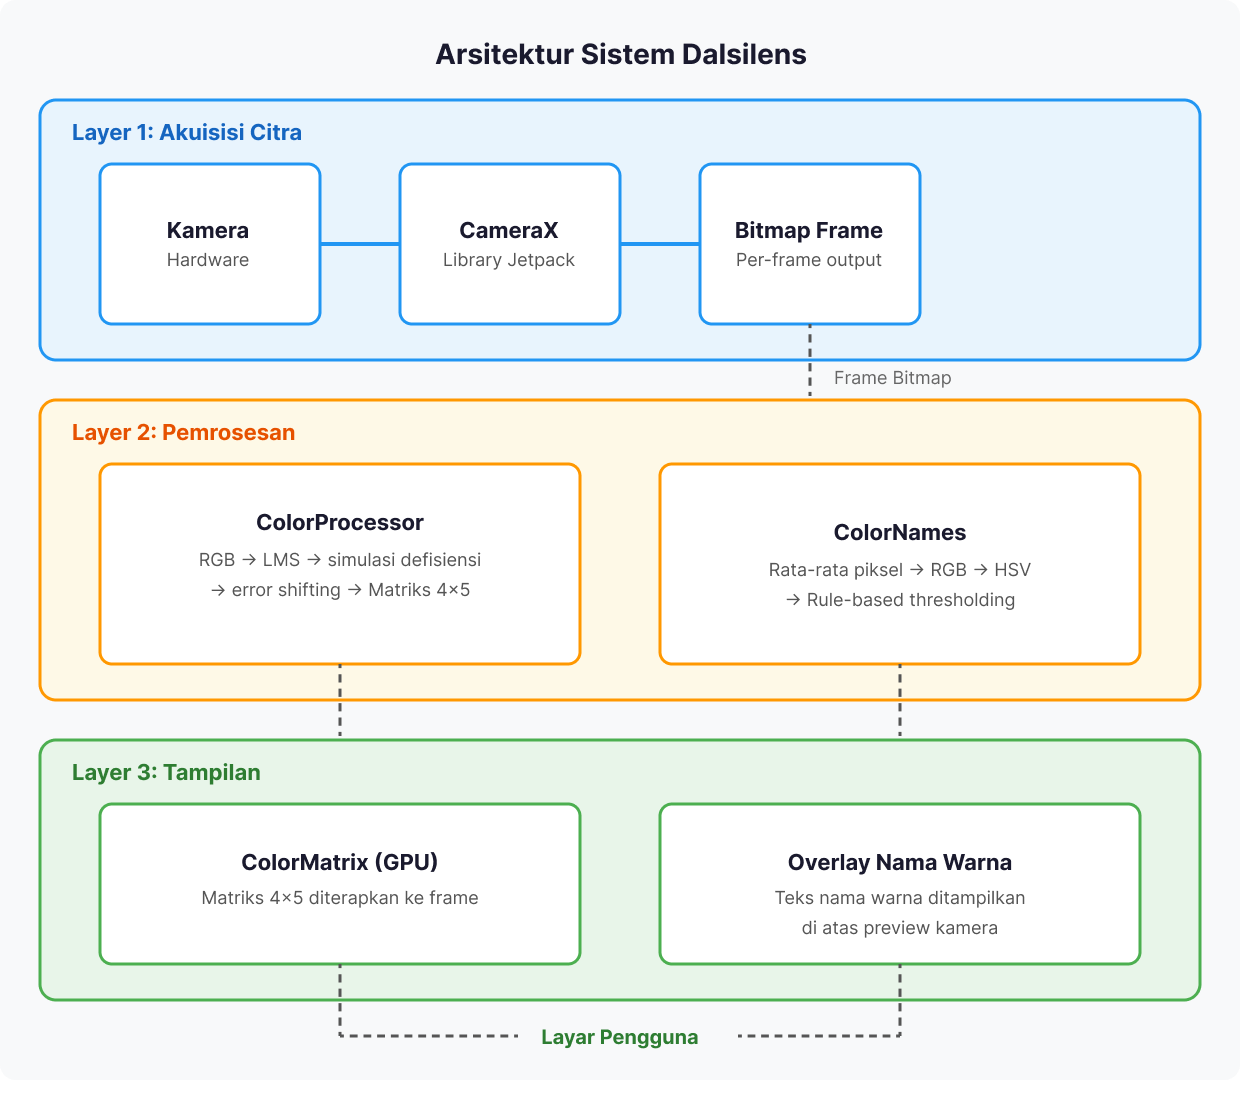
\includegraphics[width=\linewidth]{arsitektur-umum}\\[0.3em]
  {\footnotesize\textit{Gambar 1. Arsitektur Umum Sistem Dalsilens}}
\end{figure}

\subsubsection{Akuisisi Citra dan Identifikasi Warna}

\textit{Flowchart} pada Gambar 2 menggambarkan proses awal pengolahan citra yang ditangkap oleh perangkat keras kamera. Pertama, ketika pengguna mengakses antarmuka utama aplikasi, sistem secara otomatis menginisialisasi modul kamera. Selanjutnya, kamera secara terus-menerus menangkap setiap \textit{frame} dan meneruskannya ke komponen \textit{ImageAnalysis}. Citra yang diterima komponen ini kemudian dikonversi menjadi representasi \textit{bitmap} mentah untuk diproses lebih lanjut oleh memori sistem. Setelah proses konversi selesai, sistem menentukan area atau \textit{Region of Interest} (ROI) tertentu yang berada tepat di tengah \textit{bitmap}, merepresentasikan objek yang menjadi target \textit{crosshair}. Sistem mengekstrak sekumpulan piksel dalam ROI tersebut untuk dianalisis. Piksel yang diekstrak kemudian dirata-ratakan untuk memperoleh nilai RGB representatif, yang selanjutnya dikonversi ke ruang warna HSV. Nilai HSV yang dihasilkan kemudian diklasifikasikan menggunakan pendekatan \textit{rule-based thresholding} untuk menentukan warna dominan pada area target. Pada tahap akhir, \textit{bitmap} mentah dan label warna dominan yang dihasilkan disimpan dalam variabel \textit{state}. Perubahan pada \textit{state} ini selanjutnya memicu pembaruan antarmuka secara reaktif, sehingga memungkinkan \textit{rendering} visual yang dinamis.

\begin{figure}[H]
  \centering
  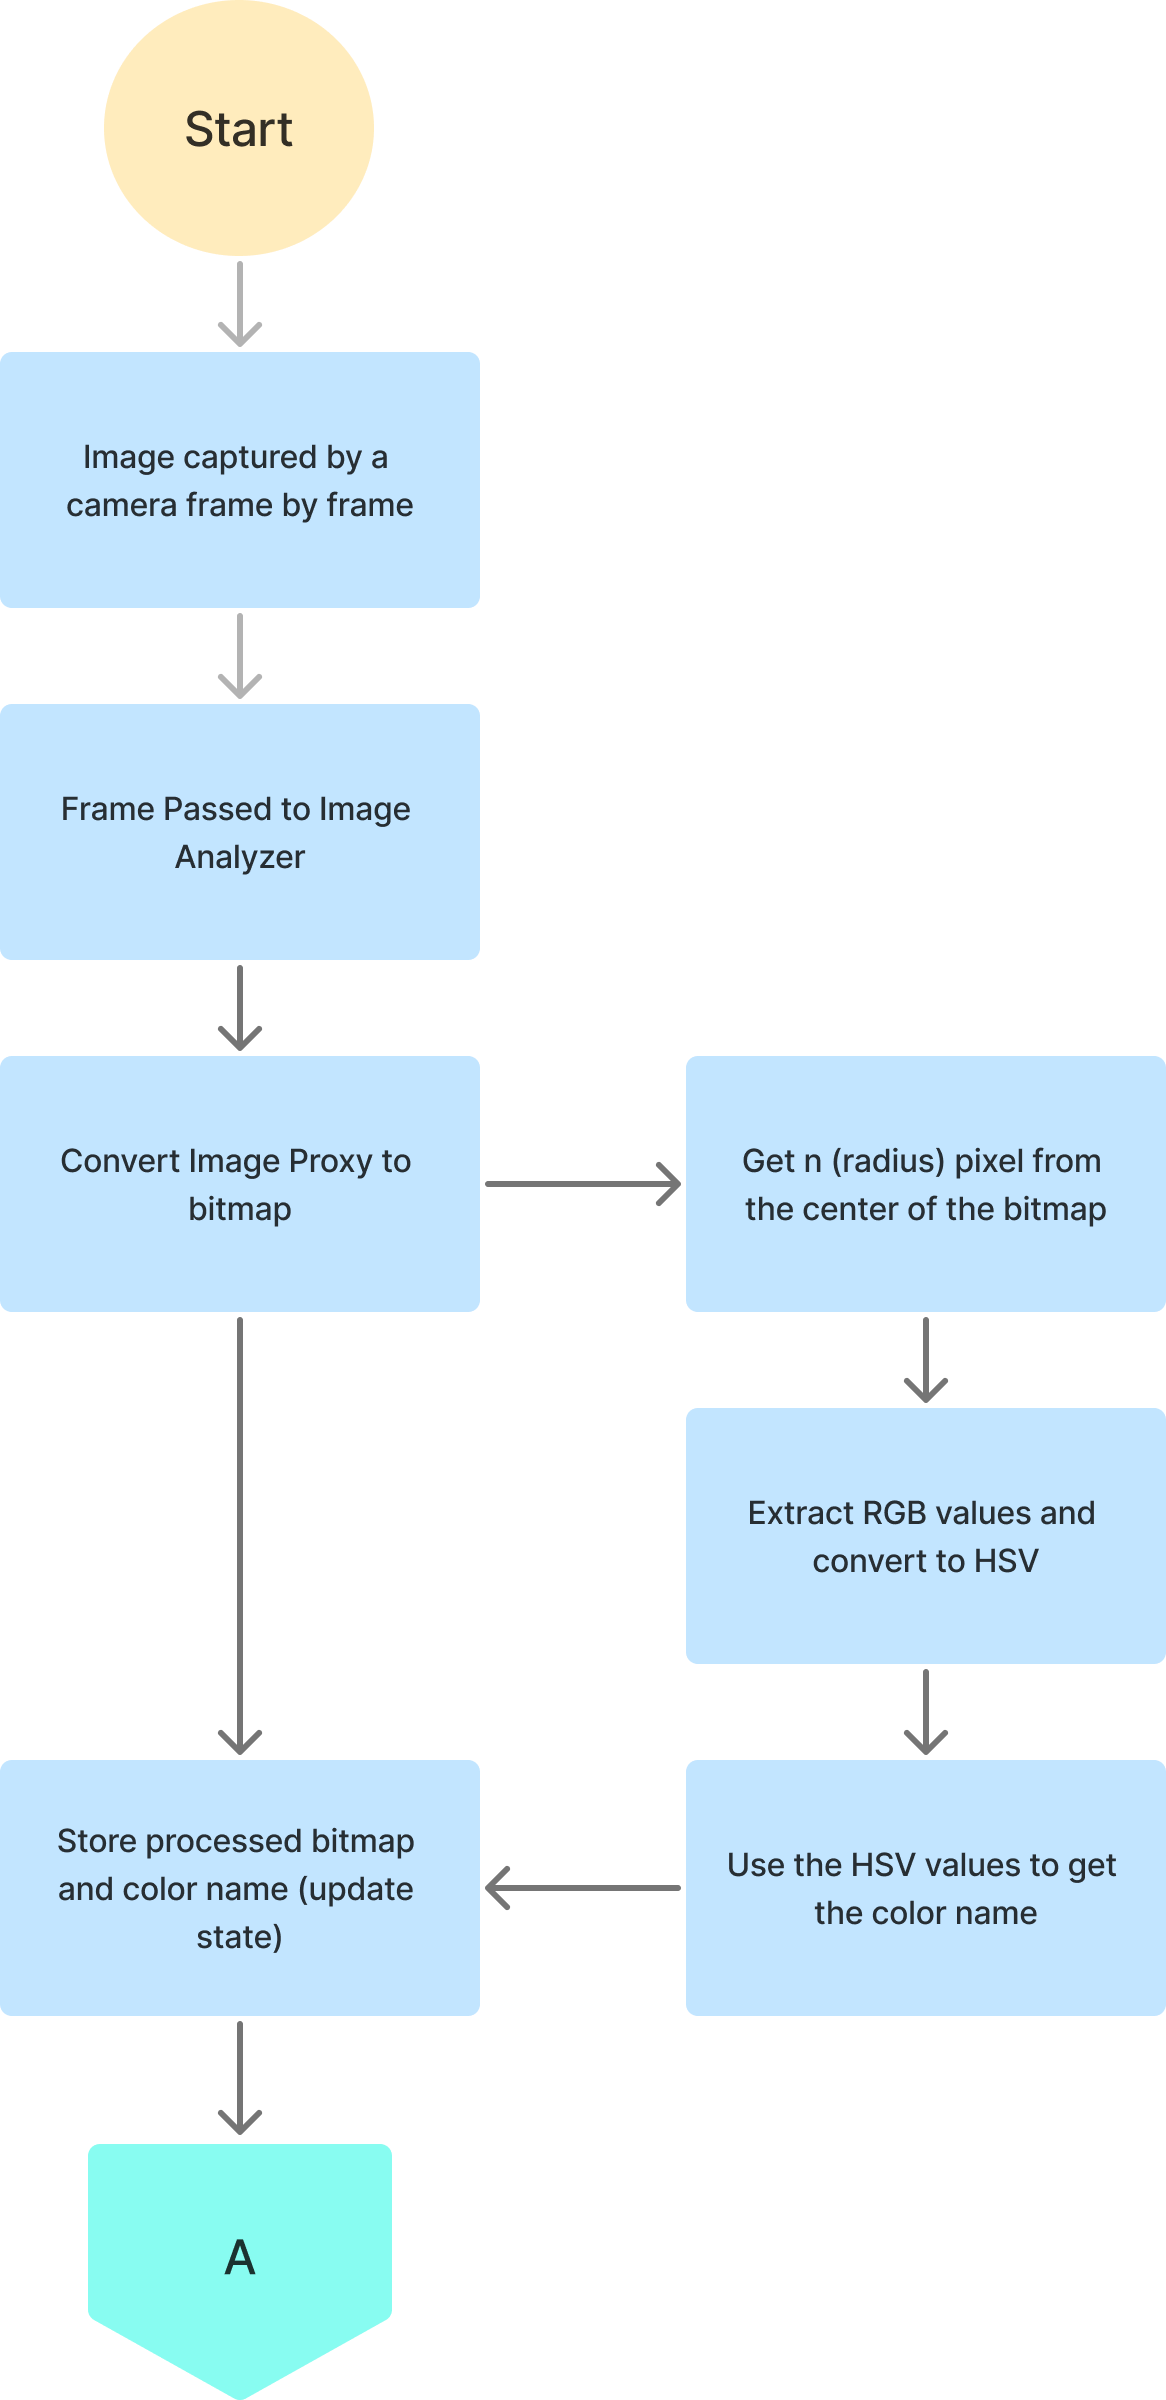
\includegraphics[width=0.8\linewidth]{flowchart-akuisisi}\\[0.3em]
  {\footnotesize\textit{Gambar 2. Flowchart Akuisisi Citra dan Identifikasi Warna}}
\end{figure}

\subsubsection{Proses Daltonisasi}

Berdasarkan \textit{flowchart} pada Gambar 3, setelah \textit{bitmap} dan label warna diperoleh dan disimpan, sistem memicu mekanisme pembaruan reaktif untuk memperbarui antarmuka pengguna. Perubahan pada label warna yang terdeteksi langsung tercermin pada antarmuka, sementara \textit{bitmap} menjalani tahap verifikasi untuk menentukan apakah filter telah diaktifkan. Jika filter tidak diaktifkan, sistem menerapkan matriks warna identitas untuk mempertahankan representasi warna asli citra. Sebaliknya, jika filter diaktifkan, transformasi matriks warna diterapkan sesuai dengan model simulasi buta warna yang dipilih. Selanjutnya, ketika fitur daltonisasi diaktifkan, citra diproses lebih lanjut menggunakan algoritma daltonisasi berbasis LMS untuk meningkatkan persepsi warna. \textit{Bitmap} dan matriks warna yang telah ditentukan kemudian diteruskan ke komponen \textit{Image}. Pada tahap ini, manipulasi warna dilakukan menggunakan \textit{Color Matrix Filter} yang dieksekusi melalui akselerasi GPU, sehingga proses \textit{rendering} dapat dilakukan secara efisien.

\begin{figure}[H]
  \centering
  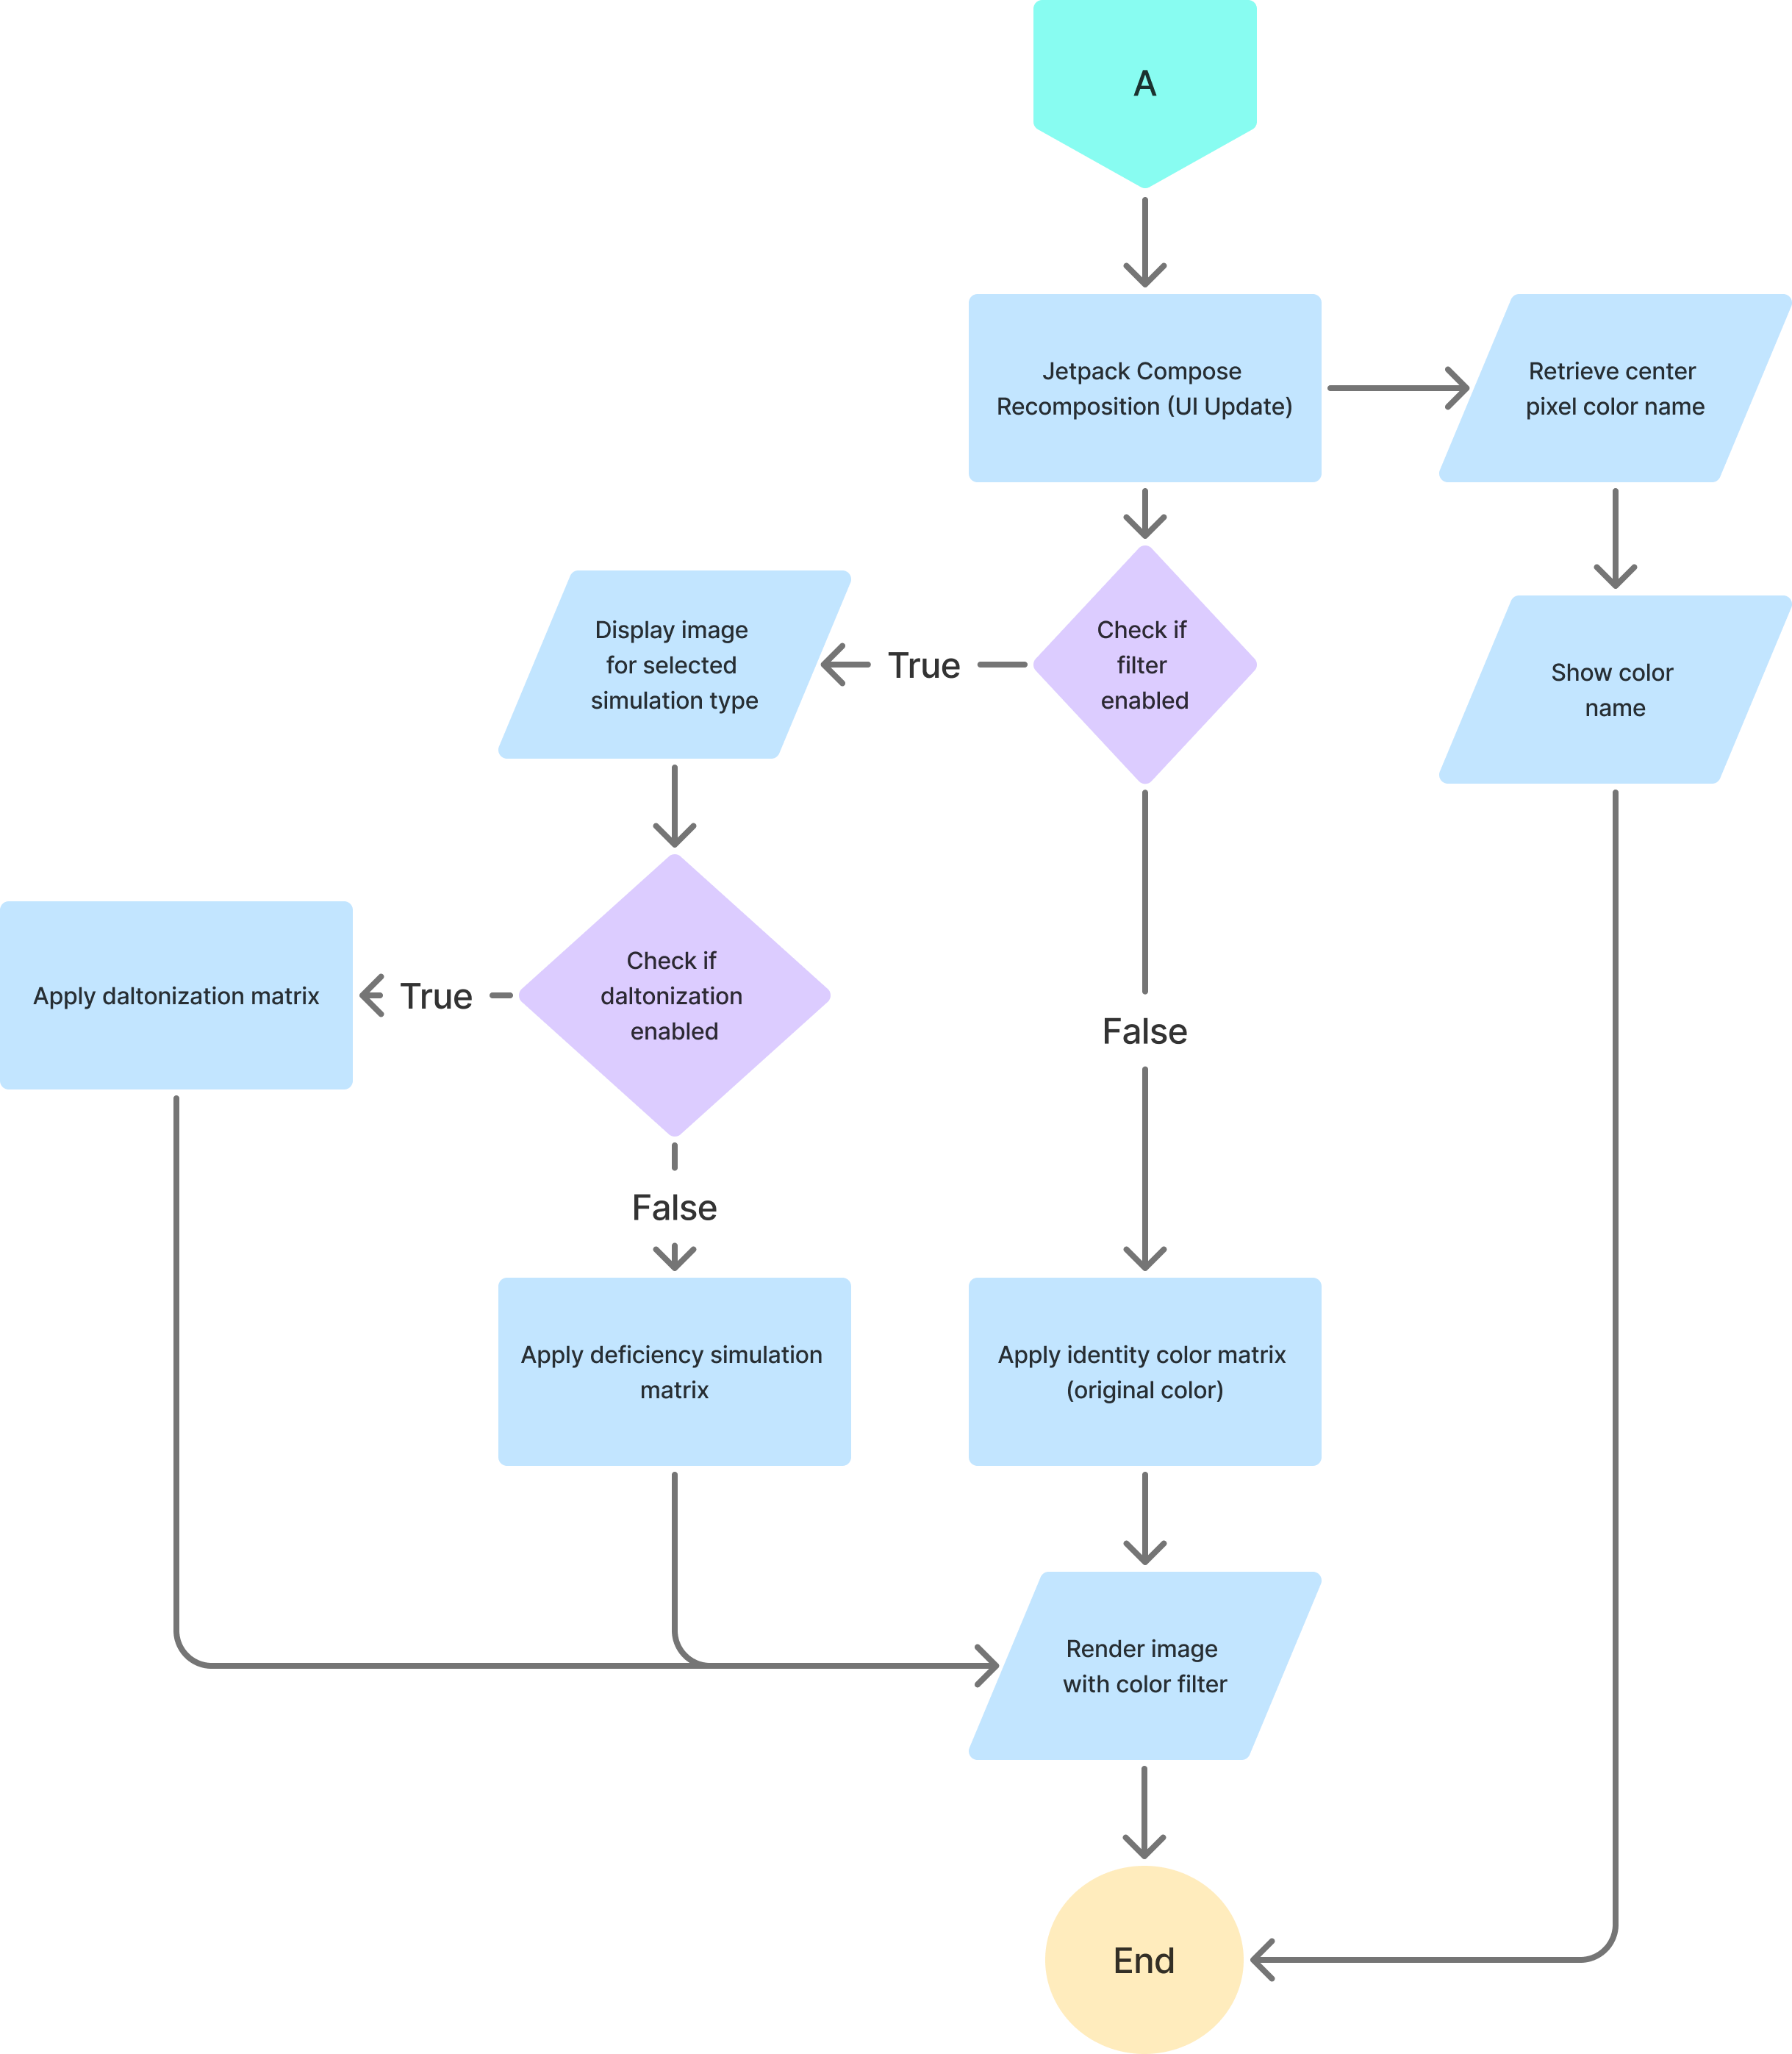
\includegraphics[width=\linewidth]{flowchart-daltonisasi}\\[0.3em]
  {\footnotesize\textit{Gambar 3. Flowchart Simulasi Defisiensi Penglihatan Warna dan Proses Daltonisasi}}
\end{figure}

\subsection{Implementasi Algoritma LMS Daltonization}

Pada bagian ini akan dibahas implementasi algoritma \textit{LMS Daltonization}, dimulai dari konversi RGB ke LMS yang merupakan ruang warna yang digunakan mata manusia untuk mempersepsikan warna, dilanjutkan dengan simulasi kondisi buta warna, hingga proses implementasi algoritma daltonisasi.

\subsubsection{Konversi Ruang Warna RGB ke LMS}

Tahap pertama dalam proses implementasi algoritma ini adalah mengonversi ruang warna citra dari RGB (\textit{Red, Green, Blue}) ke LMS (\textit{Long, Medium, Short}). Konversi ini dilakukan menggunakan transformasi linear berbasis matriks, yang merepresentasikan tiga jenis sel kerucut pada sistem penglihatan manusia. Secara matematis, transformasi ini dilakukan dengan mengalikan vektor warna RGB dengan matriks konversi tertentu, sehingga menghasilkan representasi warna pada ruang LMS. Nilai L, M, dan S dalam penelitian ini dinyatakan sebagai berikut, dengan koefisien dari [9]:

\begin{equation}
\begin{bmatrix} L \\ M \\ S \end{bmatrix} =
\begin{bmatrix} 17{,}8824 & 43{,}5161 & 4{,}11935 \\ 3{,}4565 & 27{,}1554 & 3{,}86714 \\ 0{,}02996 & 0{,}18431 & 1{,}46709 \end{bmatrix}
\begin{bmatrix} R \\ G \\ B \end{bmatrix}
\end{equation}

Koefisien pada persamaan tersebut diperoleh dari [9], yang digunakan sebagai acuan dalam proses konversi warna dari ruang RGB ke LMS. Nilai-nilai ini menunjukkan hubungan antara elemen RGB dan respons setiap kanal pada ruang LMS, sehingga hasil konversi dapat diterapkan secara akurat pada tahap pemrosesan selanjutnya. Ruang warna LMS ini digunakan sebagai dasar untuk mensimulasikan defisiensi penglihatan warna dan menerapkan algoritma daltonisasi pada tahap berikutnya.

\subsubsection{Simulasi Defisiensi Penglihatan Warna}

Tahap kedua berfokus pada pemodelan matematis untuk mensimulasikan penurunan kemampuan persepsi warna berdasarkan jenis defisiensi, yaitu \textit{Protanopia}, \textit{Deuteranopia}, dan \textit{Tritanopia}. Proses ini dilakukan dengan memodifikasi nilai komponen pada ruang LMS yang diperoleh dari tahap sebelumnya. Pada kondisi ini, salah satu komponen (L, M, atau S) kehilangan sensitivitasnya dan tidak digunakan secara langsung, melainkan dihitung ulang berdasarkan kombinasi dua komponen lainnya, dengan koefisien transformasi dari [10]:

\begin{equation}
\begin{bmatrix} L_{sim} \\ M_{sim} \\ S_{sim} \end{bmatrix}_{Prot} =
\begin{bmatrix} 0 & 2{,}02344 & -2{,}52581 \\ 0 & 1 & 0 \\ 0 & 0 & 1 \end{bmatrix}
\begin{bmatrix} L \\ M \\ S \end{bmatrix}
\end{equation}

\begin{equation}
\begin{bmatrix} L_{sim} \\ M_{sim} \\ S_{sim} \end{bmatrix}_{Deut} =
\begin{bmatrix} 1 & 0 & 0 \\ 0{,}49421 & 0 & 1{,}24827 \\ 0 & 0 & 1 \end{bmatrix}
\begin{bmatrix} L \\ M \\ S \end{bmatrix}
\end{equation}

\begin{equation}
\begin{bmatrix} L_{sim} \\ M_{sim} \\ S_{sim} \end{bmatrix}_{Trit} =
\begin{bmatrix} 1 & 0 & 0 \\ 0 & 1 & 0 \\ -0{,}39591 & 0{,}80111 & 0 \end{bmatrix}
\begin{bmatrix} L \\ M \\ S \end{bmatrix}
\end{equation}

Koefisien pada ketiga persamaan tersebut diperoleh dari [10], [16], yang digunakan untuk menyesuaikan perubahan komponen warna sesuai jenis defisiensi yang disimulasikan. Dengan cara ini, hasil simulasi dapat menunjukkan bagaimana warna tampak bagi pengguna dengan defisiensi penglihatan warna tertentu.

Hasil dari tahap ini berupa nilai LMS yang telah dimodifikasi untuk mensimulasikan kondisi penglihatan pada defisiensi warna. Nilai tersebut kemudian dikonversi kembali ke ruang RGB menggunakan matriks kebalikan (\textit{inverse}) dari Persamaan (1), untuk merepresentasikan bagaimana warna terlihat oleh penyandang buta warna, sekaligus mengamati perubahan hasil setelah penerapan algoritma daltonisasi:

\begin{equation}
\resizebox{0.95\linewidth}{!}{$\displaystyle
\begin{bmatrix} R_{sim} \\ G_{sim} \\ B_{sim} \end{bmatrix} =
\begin{bmatrix} 0{,}08094 & -0{,}13050 & 0{,}11672 \\ -0{,}01025 & 0{,}05402 & -0{,}11362 \\ -0{,}00037 & -0{,}00412 & 0{,}69351 \end{bmatrix}
\begin{bmatrix} L_{sim} \\ M_{sim} \\ S_{sim} \end{bmatrix}$}
\end{equation}

\subsubsection{Proses Daltonisasi}

Pada tahap ini, proses daltonisasi dilakukan dengan menghitung selisih antara warna asli dan warna hasil simulasi defisiensi warna. Perhitungan dimulai dengan mengonversi nilai warna dari ruang RGB ke LMS, mensimulasikan defisiensi warna pada ruang LMS, kemudian mengonversinya kembali ke ruang RGB. Selisih warna asli terhadap warna hasil simulasi kemudian dihitung sebagai nilai galat (\textit{error}):

\begin{equation}
E_R = R - R_{sim}, \quad E_G = G - G_{sim}, \quad E_B = B - B_{sim}
\end{equation}

Setelah nilai galat diperoleh, langkah berikutnya adalah mendistribusikan ulang nilai tersebut ke komponen warna lain melalui proses \textit{error shifting}. Proses ini dilakukan karena komponen warna yang terpengaruh oleh defisiensi tidak dapat dipersepsikan secara optimal oleh pengguna, sehingga informasi warna yang hilang perlu dialihkan ke komponen warna lain yang masih dapat dibedakan. Redistribusi ini dilakukan menggunakan matriks transformasi yang berbeda untuk setiap jenis defisiensi, guna menyesuaikan arah distribusi galat ke komponen warna yang masih dapat dipersepsikan secara optimal.

Pada kondisi \textit{Protanopia}, komponen merah mengalami penurunan sensitivitas sehingga tidak menerima distribusi galat, dan seluruh galat dialihkan ke komponen hijau dan biru. Pada \textit{Deuteranopia}, komponen hijau merupakan komponen yang paling terpengaruh sehingga tidak digunakan dalam redistribusi, dan galat dialihkan ke komponen merah dan biru. Sedangkan pada \textit{Tritanopia}, komponen biru mengalami penurunan sensitivitas, sehingga galat dialihkan ke komponen merah dan hijau. Koefisien ketiga matriks berikut diperoleh dari [8], [10], [16]:

\begin{equation}
\begin{bmatrix} R_{shift} \\ G_{shift} \\ B_{shift} \end{bmatrix}_{Prot} =
\begin{bmatrix} 0 & 0 & 0 \\ 0{,}7 & 1 & 0 \\ 0{,}7 & 0 & 1 \end{bmatrix}
\begin{bmatrix} E_R \\ E_G \\ E_B \end{bmatrix}
\end{equation}

\begin{equation}
\begin{bmatrix} R_{shift} \\ G_{shift} \\ B_{shift} \end{bmatrix}_{Deut} =
\begin{bmatrix} 1 & 0{,}7 & 0 \\ 0 & 0 & 0 \\ 0 & 0{,}7 & 1 \end{bmatrix}
\begin{bmatrix} E_R \\ E_G \\ E_B \end{bmatrix}
\end{equation}

\begin{equation}
\begin{bmatrix} R_{shift} \\ G_{shift} \\ B_{shift} \end{bmatrix}_{Trit} =
\begin{bmatrix} 1 & 0 & 0{,}7 \\ 0 & 1 & 0{,}7 \\ 0 & 0 & 0 \end{bmatrix}
\begin{bmatrix} E_R \\ E_G \\ E_B \end{bmatrix}
\end{equation}

Nilai galat yang telah digeser kemudian dijumlahkan kembali dengan warna asli untuk menghasilkan warna hasil koreksi (daltonisasi):

\begin{equation}
R_{d} = R + R_{shift}, \; G_{d} = G + G_{shift}, \; B_{d} = B + B_{shift}
\end{equation}

\subsubsection{Konstruksi Matriks Transformasi 4$\times$5}

Pada tahap ini, seluruh proses transformasi warna yang telah dijelaskan sebelumnya direpresentasikan sebagai fungsi transformasi $T(R,G,B)$. Untuk mengoptimalkan beban komputasi dan menghindari kalkulasi piksel yang berulang, fungsi transformasi ini disederhanakan menjadi sebuah matriks konstan berukuran 4$\times$5. Penyederhanaan dilakukan dengan mengevaluasi fungsi $T$ terhadap tiga vektor warna primer, yaitu merah murni $(1,0,0)$, hijau murni $(0,1,0)$, dan biru murni $(0,0,1)$:

\begin{equation}
\begin{aligned}
T(1,0,0) &= (r_R, r_G, r_B) \\
T(0,1,0) &= (g_R, g_G, g_B) \\
T(0,0,1) &= (b_R, b_G, b_B)
\end{aligned}
\end{equation}

Nilai hasil transformasi ketiga vektor basis tersebut kemudian disusun ke dalam kolom-kolom koefisien matriks $M_{dalton}$, sehingga matriks ini dapat langsung memetakan profil warna asli menjadi warna hasil koreksi, sekaligus mempertahankan parameter \textit{alpha} (transparansi) pada baris keempat:

\begin{equation}
M_{dalton} =
\begin{bmatrix}
r_R & g_R & b_R & 0 & 0 \\
r_G & g_G & b_G & 0 & 0 \\
r_B & g_B & b_B & 0 & 0 \\
0 & 0 & 0 & 1 & 0
\end{bmatrix}
\end{equation}

Matriks $M_{dalton}$ inilah yang langsung diterapkan pada \textit{ColorMatrix} Android dan dieksekusi melalui akselerasi GPU, sehingga tidak diperlukan kalkulasi ulang Persamaan (1) hingga (10) pada setiap piksel citra secara \textit{real-time}.

\subsection{Implementasi Tingkat Keparahan (Severity Level)}

Bagian ini menjelaskan bagaimana penyesuaian tingkat keparahan defisiensi warna diimplementasikan secara dinamis. Parameter \textit{severity} direpresentasikan dalam rentang desimal 0,0 hingga 1,0. Untuk menjaga akurasi representasi visual, sistem membedakan metode penerapan \textit{severity} berdasarkan tujuannya, yaitu antara proses simulasi penglihatan dan proses daltonisasi.

\subsubsection{Pemodelan Severity pada Simulasi Defisiensi}

Pada mode simulasi, parameter \textit{severity} berfungsi untuk meniru tingkat kerusakan atau pergeseran sensitivitas pada sel kerucut mata pengguna. Proses ini mendekati suatu kondisi medis yang dikenal sebagai \textit{Anomalous Trichromacy} [11]. Oleh karena itu, perhitungan dilakukan secara langsung pada ruang warna LMS menggunakan metode interpolasi linear. Sistem menghitung selisih antara nilai LMS pada kondisi penglihatan normal dan nilai LMS pada kondisi defisiensi penuh, kemudian selisih tersebut dikalikan dengan parameter \textit{severity} dan dijumlahkan kembali ke nilai normal:

\begin{equation}
L_{f} = L_{n} + (L_{sim} - L_{n}) \times S
\end{equation}

\subsubsection{Pemodelan Severity pada Koreksi Penglihatan Warna}

Berbeda dari tahap simulasi, parameter \textit{severity} pada proses daltonisasi berfungsi untuk menentukan intensitas atau kekuatan bantuan warna yang diberikan kepada pengguna. Perhitungan ini dilakukan pada ruang warna RGB, tepatnya pada tahap akhir komputasi ketika nilai galat yang telah digeser ditambahkan ke piksel asli. Intensitas kompensasi warna disesuaikan dengan mengalikan hasil galat yang telah digeser dari setiap kanal warna dengan nilai \textit{severity}, sebelum digabungkan dengan warna asli, sehingga pengguna dapat menyesuaikan kontras warna secara proporsional sesuai kenyamanan visualnya:

\begin{equation}
R_{d} = R + (R_{shift} \times S)
\end{equation}

\subsection{Ekstraksi Warna Dominan Berbasis Ruang Warna HSV}

Pada bagian ini akan dibahas proses ekstraksi warna dominan berdasarkan ruang warna HSV. Tahap ini bertujuan mengekstrak warna dari objek yang berada pada titik tengah yang menjadi target \textit{crosshair} secara \textit{real-time}. Proses ini dimulai dengan memperoleh citra dalam bentuk \textit{bitmap}, dilanjutkan dengan pemrosesan area piksel di sekitar titik tengah, dan diakhiri dengan klasifikasi nama warna menggunakan ruang warna HSV.

\subsubsection{Akuisisi dan Pemrosesan Bitmap}

\textit{Frame} dari kamera diperoleh melalui \textit{ImageAnalysis} pada \textit{CameraX}, yang secara terus-menerus menangkap citra. \textit{Frame} tersebut kemudian diteruskan ke fungsi \textit{analyzer}, yang menghasilkan \textit{ImageProxy}, sebelum akhirnya dikonversi menjadi \textit{Bitmap}. Mengingat orientasi sensor kamera bervariasi antar perangkat Android, nilai \texttt{rotationDegrees} pada metadata \textit{frame} diperiksa. Apabila nilai rotasi tidak sama dengan nol, \textit{bitmap} akan dirotasi menggunakan matriks transformasi.

\subsubsection{Pengambilan Sampel Piksel}

Pengambilan sampel warna tidak hanya dilakukan pada satu titik piksel di tengah layar, karena sampel satu piksel cenderung kurang efektif akibat warna pada suatu area dapat dipengaruhi oleh gangguan (\textit{noise}), pencahayaan, atau kondisi lainnya. Oleh karena itu, digunakan pendekatan \textit{sampling} dengan mengambil beberapa piksel di sekitar titik tengah, sehingga warna yang diperoleh menjadi lebih stabil dan dapat merepresentasikan warna dominan pada area yang diamati dengan lebih baik.

Langkah pertama adalah menentukan radius area \textit{sampling}, dengan nilai radius \textit{default} sebesar $r=5$. Dengan radius tersebut, area sampel yang diambil mencakup 121 piksel (11 x 11). Jumlah piksel yang digunakan dapat dihitung menggunakan persamaan berikut:

\begin{equation}
N = (2r+1) \times (2r+1)
\end{equation}

Diberikan citra $I$ berukuran $W \times H$ dan titik tengah $(x_c, y_c)$ dengan radius $r$, sebuah fungsi pembatas (\textit{bounding function}) didefinisikan agar koordinat piksel yang diproses tidak melampaui batas citra:

\begin{equation}
f(x) = \min(\max(x, 0), W-1)
\end{equation}
\begin{equation}
g(y) = \min(\max(y, 0), H-1)
\end{equation}

Setiap piksel pada koordinat $(x,y)$ disimpan sebagai bilangan bulat 32-bit berformat ARGB. Struktur bit dari komponen biru (B) berada pada posisi paling akhir, sehingga tidak diperlukan pergeseran bit, cukup dilakukan \textit{masking} untuk menghilangkan bit lainnya menggunakan nilai \textit{mask} 255 (0xFF). Sementara itu, komponen hijau (G) berada pada posisi tengah sehingga perlu digeser ke kanan sebanyak delapan bit terlebih dahulu, dan komponen merah (R) berada pada posisi paling kiri sehingga perlu digeser ke kanan sebanyak 16 bit. Ketiga komponen warna tersebut diekstrak melalui operasi pergeseran bit (\textit{bit shift}) dan \textit{masking} terhadap nilai piksel:

\begin{equation}
B_{(x,y)} = \text{pixel} \mathbin{\&} 255
\end{equation}
\begin{equation}
G_{(x,y)} = (\text{pixel} \gg 8) \mathbin{\&} 255
\end{equation}
\begin{equation}
R_{(x,y)} = (\text{pixel} \gg 16) \mathbin{\&} 255
\end{equation}

Nilai RGB rata-rata dari seluruh $N$ piksel dalam area sampel kemudian dihitung sebagai representasi warna dominan:

\begin{equation}
\bar{R} = \frac{1}{N}\sum_{i=1}^{N} R_i, \quad
\bar{G} = \frac{1}{N}\sum_{i=1}^{N} G_i, \quad
\bar{B} = \frac{1}{N}\sum_{i=1}^{N} B_i
\end{equation}

\subsubsection{Klasifikasi Nama Warna}

Tahap akhir adalah klasifikasi warna, yang dilakukan dengan mengonversi nilai RGB rata-rata yang diperoleh ke ruang warna HSV menggunakan fungsi bawaan Android pada kelas \texttt{android.graphics.Color}, yaitu \texttt{RGBToHSV(r, g, b, hsv)}. Hasil konversi terdiri dari tiga komponen, yaitu \textit{Hue} (H) sebagai jenis warna pada rentang $0^\circ$--$360^\circ$, \textit{Saturation} (S) sebagai tingkat intensitas warna pada rentang 0 hingga 1, dan \textit{Value} (V) sebagai tingkat kecerahan pada rentang 0 hingga 1. Ketiga komponen ini kemudian digunakan untuk menentukan nama warna menggunakan pendekatan \textit{threshold} berdasarkan rentang nilai H, S, dan V. Nilai \textit{threshold} ditentukan melalui pengujian sampel warna pada kondisi pencahayaan normal dan redup, dengan mempertimbangkan nilai rata-rata, simpangan baku, dan rentang toleransi.

Sebagai contoh, berikut perhitungan untuk menentukan rentang nilai H bagi warna merah. Data uji diperoleh dari 10 sampel pada kondisi pencahayaan normal dan 10 sampel pada kondisi pencahayaan redup, yang kemudian digunakan untuk menghitung nilai rata-rata dan rentang variasi komponen \textit{Hue}. Hasil perhitungan menunjukkan bahwa nilai rata-rata komponen \textit{Hue} pada kondisi pencahayaan normal adalah $3,3^\circ$, sedangkan pada kondisi pencahayaan redup adalah $8,1^\circ$. Selanjutnya, dihitung simpangan baku untuk mengetahui sebaran data pada masing-masing kondisi, dan diperoleh nilai simpangan baku sebesar $0,48^\circ$ pada kondisi normal dan $0,88^\circ$ pada kondisi redup.

Nilai toleransi (batas atas dan bawah) kemudian ditentukan dengan menjumlahkan dan mengurangkan nilai rata-rata dengan simpangan baku, menggunakan persamaan $\bar{H} \pm 2\sigma$. Batas bawah untuk kondisi pencahayaan normal diperoleh dari $3,3 - 2(0,48^\circ) = 2,34^\circ$, sedangkan batas atas diperoleh dari $3,3 + 2(0,48^\circ) = 4,26^\circ$, sehingga rentang toleransi pada kondisi normal berada di antara $2,34^\circ$ dan $4,26^\circ$. Metode yang sama diterapkan pada kondisi redup, dengan batas bawah $8,1 - 2(0,88^\circ) = 6,34^\circ$ dan batas atas $8,1 + 2(0,88^\circ) = 9,86^\circ$, sehingga rentang toleransi pada kondisi redup berada di antara $6,34^\circ$ dan $9,86^\circ$.

Apabila dibandingkan, rentang nilai \textit{Hue} dari kondisi normal dan redup tidak menunjukkan tumpang tindih (\textit{overlap}). Berdasarkan hasil ini, penentuan nilai \textit{threshold} dilakukan dengan menetapkan batas atas dari kondisi dengan variasi terbesar, yaitu $9,86^\circ$, sehingga nilai \textit{threshold} untuk warna merah dinyatakan sebagai H $< 9,86^\circ$. Metode yang sama diterapkan pada warna lainnya, sehingga menghasilkan tabel \textit{threshold} yang dapat langsung digunakan pada proses klasifikasi warna, sebagaimana ditunjukkan pada Tabel 1.

\begin{table}[H]
  \centering
  {\footnotesize
  \begin{tabular}{|c|c|}
    \hline
    \textbf{Rentang Hue ($^\circ$)} & \textbf{Kategori Warna} \\
    \hline
    H $<$ 9,85 & Merah \\ \hline
    9,85 $\leq$ H $<$ 26,98 & Oranye \\ \hline
    26,98 $\leq$ H $<$ 50,42 & Kuning \\ \hline
    50,42 $\leq$ H $<$ 122,50 & Hijau \\ \hline
    122,50 $\leq$ H $<$ 204,85 & Cyan \\ \hline
    204,85 $\leq$ H $<$ 224,57 & Biru \\ \hline
    224,57 $\leq$ H $<$ 319,37 & Ungu \\ \hline
    H $\geq$ 319,37 & Merah \\ \hline
  \end{tabular}}\\[0.3em]
  {\footnotesize\textit{Tabel 1. Klasifikasi Warna Berdasarkan Rentang Hue}}
\end{table}

Warna dengan nilai \textit{Saturation} yang rendah tidak diklasifikasikan menggunakan \textit{Hue} karena cenderung bersifat akromatik (\textit{grayscale}), sehingga klasifikasinya beralih menggunakan nilai \textit{Value} untuk membedakan kategori Hitam, Abu-abu Gelap, Abu-abu, dan Putih, sebagaimana ditunjukkan pada Tabel 2.

\begin{table}[H]
  \centering
  {\footnotesize
  \begin{tabular}{|c|c|c|}
    \hline
    \textbf{Saturation} & \textbf{Value} & \textbf{Kategori} \\
    \hline
    S $<$ 0,10 & V $<$ 0,15 & Hitam \\ \hline
    S $<$ 0,10 & 0,15 $\leq$ V $<$ 0,40 & Abu-abu Gelap \\ \hline
    S $<$ 0,10 & 0,40 $\leq$ V $<$ 0,78 & Abu-abu \\ \hline
    S $<$ 0,10 & V $\geq$ 0,78 & Putih \\ \hline
  \end{tabular}}\\[0.3em]
  {\footnotesize\textit{Tabel 2. Klasifikasi Warna Akromatik Berdasarkan Saturation dan Value}}
\end{table}

Dengan menggabungkan klasifikasi berbasis \textit{Hue}, \textit{Saturation}, dan \textit{Value}, sistem mampu mengenali warna kromatik maupun akromatik secara \textit{real-time}, meskipun kondisi pencahayaan lingkungan bervariasi.

\subsection{Skenario Pengujian}

Pengujian aplikasi mencakup empat skenario, yaitu (1) pengujian fungsionalitas menggunakan \textit{Black Box Testing} [12] terhadap 15 skenario penggunaan; (2) pengujian akurasi klasifikasi nama warna terhadap 10 kategori warna pada kondisi pencahayaan normal dan redup; (3) pengujian performa \textit{real-time} berupa FPS, latensi, penggunaan RAM, dan utilisasi CPU menggunakan \texttt{adb shell dumpsys} dan \textit{Android Studio Profiler}; serta (4) pengujian kebergunaan menggunakan kuesioner \textit{System Usability Scale} (SUS) [13] terhadap 18 responden.

% ============================================================
% 4. HASIL DAN PEMBAHASAN
% ============================================================
\section{Hasil dan Pembahasan}

\subsection{Pengujian Fungsionalitas}

Pengujian \textit{Black Box Testing} [12] dilakukan terhadap 15 skenario yang mencakup navigasi antarmuka, aktivasi/nonaktivasi filter, pemilihan jenis simulasi (\textit{Protanopia}, \textit{Deuteranopia}, \textit{Tritanopia}), pengaturan \textit{severity}, pengaturan ukuran area \textit{sampling}, serta deteksi nama warna secara \textit{real-time}. Setiap skenario diuji dengan memberikan masukan tertentu dan memverifikasi kesesuaian keluaran terhadap ekspektasi yang dirancang, mulai dari navigasi antarmuka, aktivasi dan nonaktivasi filter, pemilihan ketiga jenis simulasi buta warna, pengaturan \textit{severity} pada nilai minimum dan maksimum, hingga pengaturan ukuran area \textit{sampling}. Seluruh 15 skenario tersebut menghasilkan keluaran \textbf{Berhasil}, yang menunjukkan bahwa fitur-fitur utama aplikasi berjalan sesuai dengan ekspektasi rancangan tanpa ditemukan kegagalan fungsional.

\subsection{Pengujian Akurasi Klasifikasi Warna}

Pengujian dilakukan terhadap 10 objek fisik yang mewakili setiap kategori warna, pada dua kondisi pencahayaan yaitu \textbf{normal} (cahaya ruangan standar) dan \textbf{redup} (cahaya dikurangi menggunakan tirai). Hasil deteksi nama warna dibandingkan dengan warna objek yang sebenarnya, sebagaimana ditunjukkan pada Tabel 3 dan Tabel 4.

\begin{table}[H]
  \centering
  {\scriptsize
  \begin{tabular}{|c|l|l|l|c|}
    \hline
    \textbf{No.} & \textbf{Objek} & \textbf{Asli} & \textbf{Deteksi} & \textbf{Ket.} \\
    \hline
    1 & Tali & Merah & Merah & Benar \\ \hline
    2 & Baju & Oranye & Oranye & Benar \\ \hline
    3 & Baju & Kuning & Kuning & Benar \\ \hline
    4 & Teko & Hijau & Hijau & Benar \\ \hline
    5 & Pembersih Keyboard & Cyan & Cyan & Benar \\ \hline
    6 & Gantungan Kunci & Biru & Biru & Benar \\ \hline
    7 & KTM & Ungu & Magenta & Salah \\ \hline
    8 & Tumbler & Putih & Putih & Benar \\ \hline
    9 & Celana & Hitam & Hitam & Benar \\ \hline
    10 & Gagang Jemuran & Abu-abu & Abu-abu & Benar \\ \hline
  \end{tabular}}\\[0.3em]
  {\footnotesize\textit{Tabel 3. Hasil Pengujian Klasifikasi Warna pada Pencahayaan Normal}}
\end{table}

\begin{table}[H]
  \centering
  {\scriptsize
  \begin{tabular}{|c|l|l|l|c|}
    \hline
    \textbf{No.} & \textbf{Objek} & \textbf{Asli} & \textbf{Deteksi} & \textbf{Ket.} \\
    \hline
    1 & Tali & Merah & Merah & Benar \\ \hline
    2 & Baju & Oranye & Oranye & Benar \\ \hline
    3 & Baju & Kuning & Oranye & Salah \\ \hline
    4 & Teko & Hijau & Hijau & Benar \\ \hline
    5 & Pembersih Keyboard & Cyan & Biru & Salah \\ \hline
    6 & Gantungan Kunci & Biru & Biru & Benar \\ \hline
    7 & KTM & Ungu & Merah & Salah \\ \hline
    8 & Tumbler & Putih & Abu-abu & Salah \\ \hline
    9 & Celana & Hitam & Hitam & Benar \\ \hline
    10 & Gagang Jemuran & Abu-abu & Kuning & Salah \\ \hline
  \end{tabular}}\\[0.3em]
  {\footnotesize\textit{Tabel 4. Hasil Pengujian Klasifikasi Warna pada Pencahayaan Redup}}
\end{table}

Berdasarkan Tabel 3 dan Tabel 4, akurasi deteksi pada kondisi pencahayaan normal sebesar $\frac{9}{10} \times 100\% = 90\%$, dengan satu kesalahan pada warna ungu yang terdeteksi sebagai magenta. Pada kondisi pencahayaan redup, akurasi menurun menjadi $\frac{5}{10} \times 100\% = 50\%$, sebagaimana dirangkum pada Tabel 5.

\begin{table}[H]
  \centering
  {\footnotesize
  \begin{tabular}{|l|c|c|}
    \hline
    \textbf{Kondisi Pencahayaan} & \textbf{Benar} & \textbf{Akurasi} \\
    \hline
    Normal & 9/10 & 90\% \\ \hline
    Redup & 5/10 & 50\% \\ \hline
  \end{tabular}}\\[0.3em]
  {\footnotesize\textit{Tabel 5. Rekapitulasi Akurasi Klasifikasi Nama Warna}}
\end{table}

Penurunan akurasi pada kondisi redup terjadi karena nilai \textit{Value} (V) pada ruang warna HSV menurun secara signifikan, sehingga piksel yang seharusnya terklasifikasi berwarna cenderung terdeteksi sebagai abu-abu atau hitam. Temuan ini konsisten dengan penelitian [14] yang menyatakan bahwa akurasi kolorimetri berbasis \textit{smartphone} pada ruang warna HSV sensitif terhadap kondisi pencahayaan.

\subsection{Pengujian Performa Real-Time}

Pengujian performa dilakukan pada skenario beban komputasi tertinggi, yaitu saat mode daltonisasi dan identifikasi warna berjalan bersamaan, merepresentasikan kondisi \textit{worst-case} yang mungkin terjadi. Pengujian FPS dan latensi dilakukan menggunakan data statistik \textit{rendering frame} dari perintah \texttt{adb shell dumpsys gfxinfo}, sebanyak tiga kali iterasi, masing-masing berjalan kurang lebih satu menit, sebagaimana ditunjukkan pada Tabel 6.

\begin{table}[H]
  \centering
  {\footnotesize
  \begin{tabular}{|l|c|c|c|c|}
    \hline
    \textbf{Iterasi} & \textbf{Frame} & \textbf{FPS} & \textbf{Latensi (ms)} & \textbf{Janky (\%)} \\
    \hline
    1 & 2.389 & 55,0 & 18,2 & 28,59 \\ \hline
    2 & 2.808 & 65,3 & 15,3 & 9,62 \\ \hline
    3 & 1.134 & 46,8 & 21,4 & 23,10 \\ \hline
    \textbf{Rata-rata} & \textbf{6.331} & \textbf{57,2} & \textbf{17,5} & \textbf{19,19} \\ \hline
  \end{tabular}}\\[0.3em]
  {\footnotesize\textit{Tabel 6. Hasil Pengujian FPS dan Latensi Pemrosesan}}
\end{table}

Nilai rata-rata 57,2 FPS dengan latensi 17,5 ms menunjukkan bahwa aplikasi mendekati kondisi \textit{real-time} yang mulus (60 FPS) meskipun transformasi \textit{color matrix} dan klasifikasi warna berjalan bersamaan. Data \textit{GPU Rendering Profile} menunjukkan median waktu pemrosesan GPU berada pada kisaran 5--7 ms, jauh lebih rendah dibandingkan total waktu \textit{render} per \textit{frame}, mengindikasikan bahwa transformasi warna bukan titik hambat (\textit{bottleneck}) utama.

Penggunaan memori diukur melalui \textit{Total Proportional Set Size} (PSS) menggunakan perintah \texttt{adb shell dumpsys meminfo}, sebagaimana ditunjukkan pada Tabel 7.

\begin{table}[H]
  \centering
  {\footnotesize
  \begin{tabular}{|l|c|c|}
    \hline
    \textbf{Iterasi} & \textbf{PSS (KB)} & \textbf{PSS (MB)} \\
    \hline
    1 & 223.147 & 217,92 \\ \hline
    2 & 227.867 & 222,53 \\ \hline
    3 & 220.339 & 215,18 \\ \hline
    \textbf{Rata-rata} & \textbf{223.784} & \textbf{218,54} \\ \hline
  \end{tabular}}\\[0.3em]
  {\footnotesize\textit{Tabel 7. Hasil Pengujian Penggunaan Memori (RAM)}}
\end{table}

Nilai PSS pada tiga iterasi pengujian berada dalam rentang sempit ($\pm$3,5 MB dari rata-rata) tanpa menunjukkan tren kenaikan yang konsisten antar iterasi, sehingga tidak ditemukan indikasi \textit{memory leak} pada aplikasi Dalsilens.

Utilisasi CPU diukur menggunakan perintah \texttt{adb shell top -n 2 -d 1}, dengan nilai yang dicatat berupa sampel kedua dari setiap pasangan pengukuran, sebagaimana ditunjukkan pada Tabel 8.

\begin{table}[H]
  \centering
  {\footnotesize
  \begin{tabular}{|l|c|}
    \hline
    \textbf{Iterasi} & \textbf{Utilisasi CPU (\%)} \\
    \hline
    1 & 147 \\ \hline
    2 & 148 \\ \hline
    3 & 166 \\ \hline
    \textbf{Rata-rata} & \textbf{153,67} \\ \hline
  \end{tabular}}\\[0.3em]
  {\footnotesize\textit{Tabel 8. Hasil Pengujian Utilisasi CPU}}
\end{table}

Nilai utilisasi CPU melebihi 100\% karena utilitas berbasis Linux/Android seperti \texttt{top} menghitung persentase CPU sebagai akumulasi penggunaan pada seluruh \textit{core} yang dipakai proses, bukan relatif terhadap satu \textit{core}. Perangkat uji memiliki kapasitas total CPU sebesar 800\% (8 \textit{core}), sehingga nilai rata-rata 153,67\% apabila dikonversi menjadi persentase relatif terhadap kapasitas total perangkat menghasilkan:

\begin{equation}
\text{Utilisasi CPU Relatif} = \frac{153{,}67\%}{8 \times 100\%} \times 100\% \approx 19{,}21\%
\end{equation}

Nilai ini menunjukkan bahwa aplikasi Dalsilens hanya menggunakan sekitar 19,21\% dari total kapasitas komputasi CPU perangkat meskipun menjalankan transformasi \textit{color matrix} dan klasifikasi warna secara bersamaan, membuktikan efektivitas pemindahan beban komputasi berat dari CPU ke GPU melalui \textit{ColorMatrix} [8].

\noindent
\begin{minipage}[t]{0.48\linewidth}
  \centering
  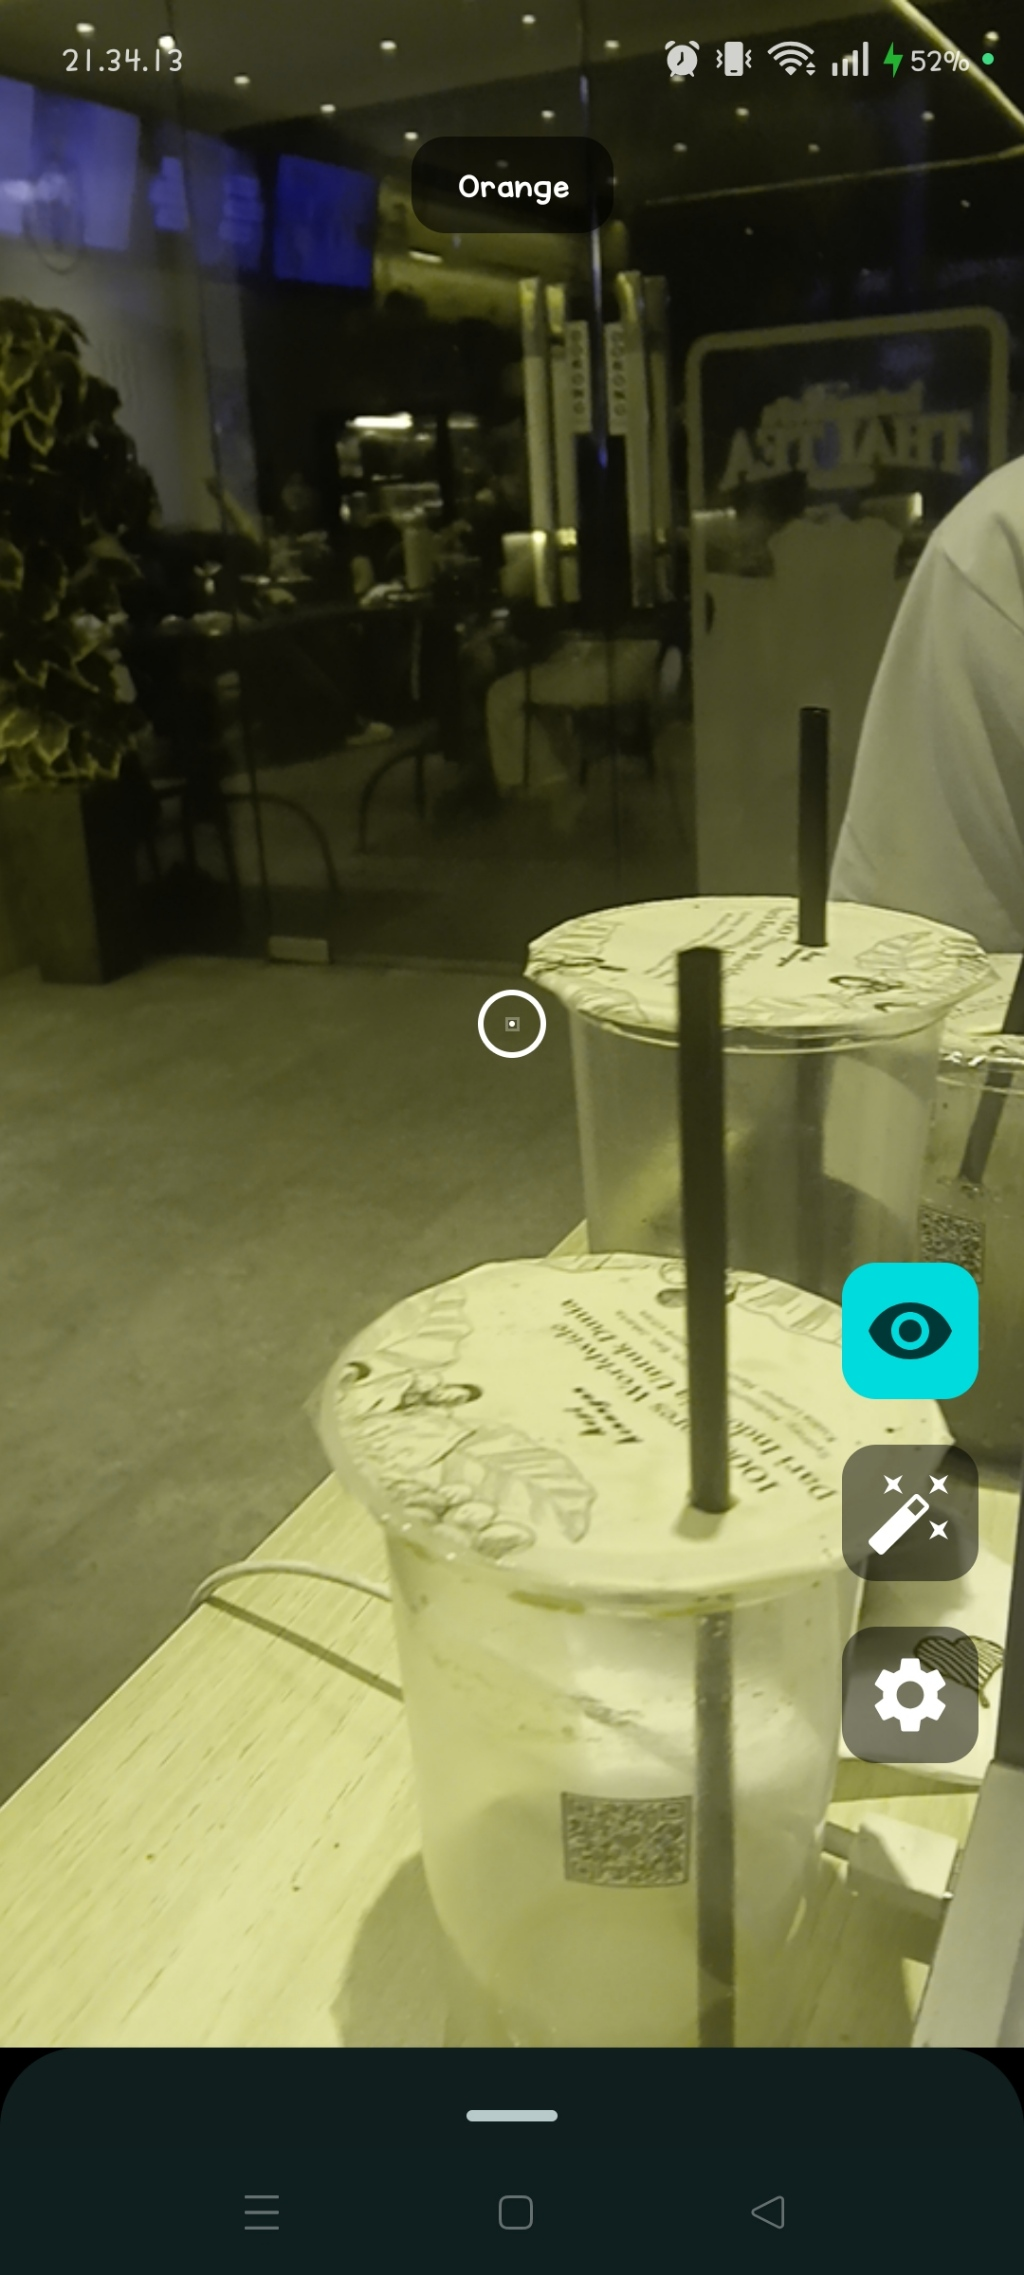
\includegraphics[width=\linewidth]{ss_deuteranopia}\\[0.2em]
  {\footnotesize\textit{Simulasi Deuteranopia}}
\end{minipage}
\hfill
\begin{minipage}[t]{0.48\linewidth}
  \centering
  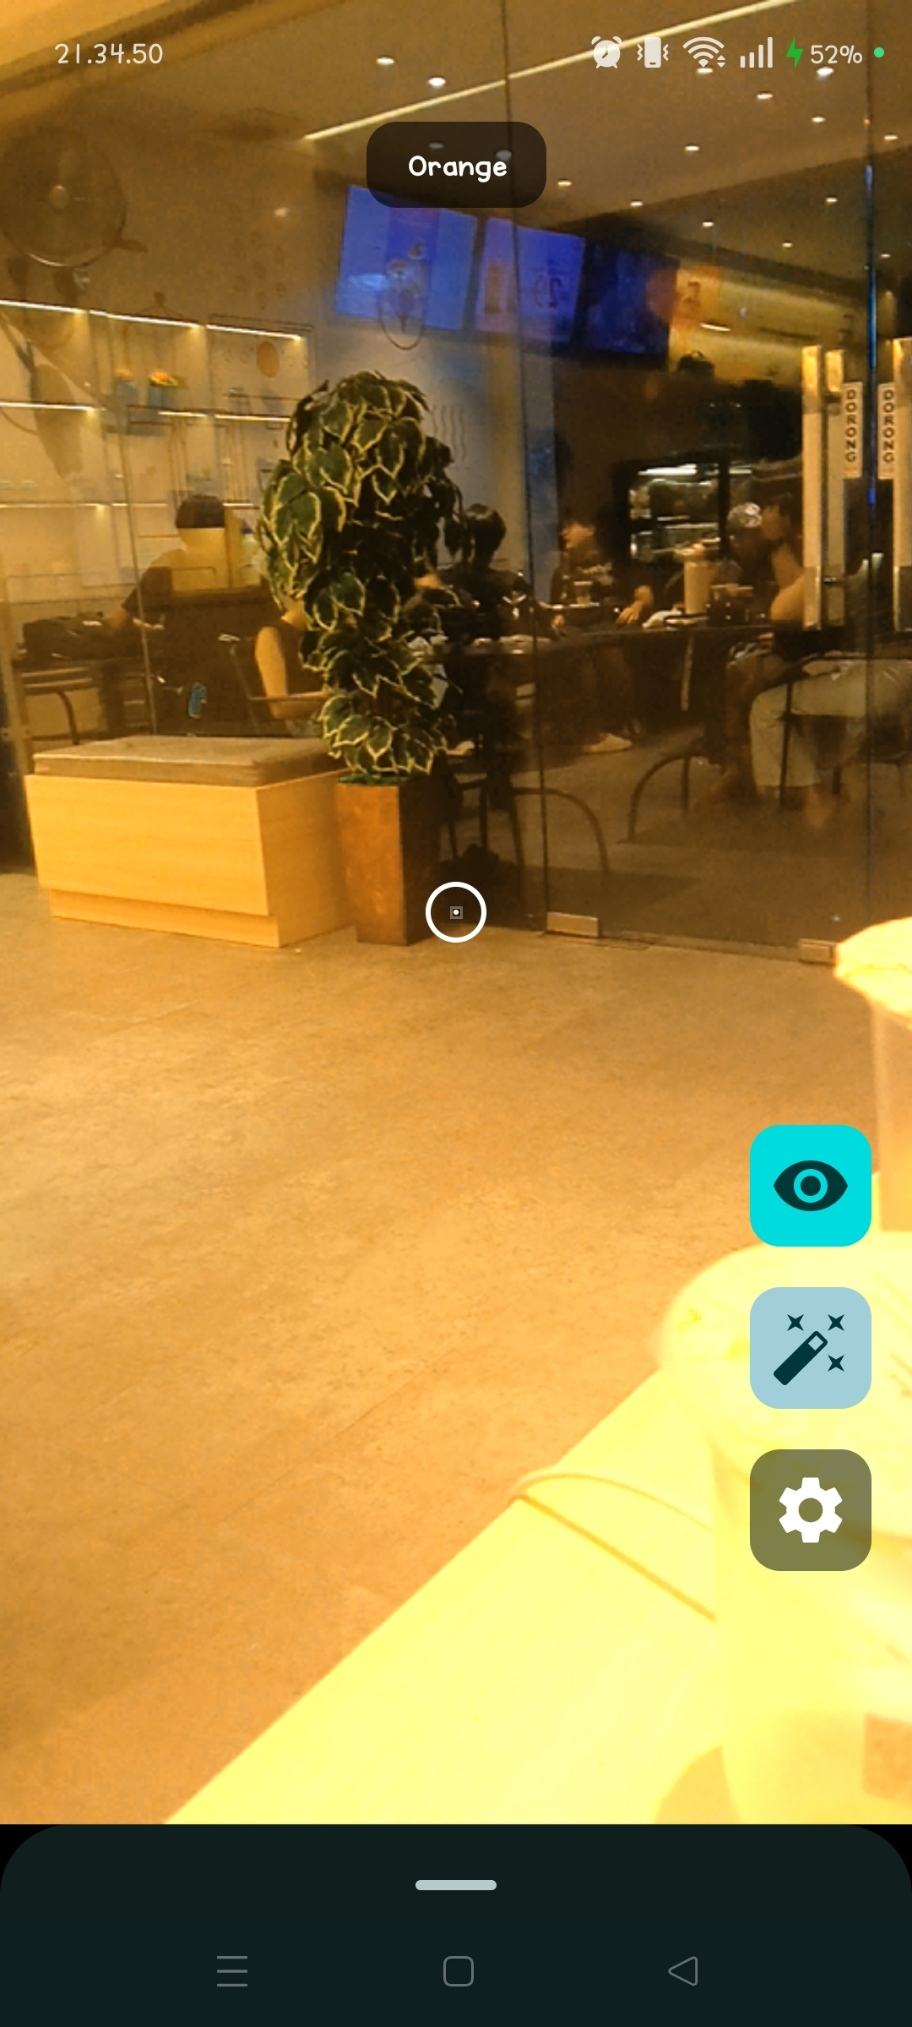
\includegraphics[width=\linewidth]{ss_daltonization}\\[0.2em]
  {\footnotesize\textit{Simulasi + Daltonisasi}}
\end{minipage}
\vspace{0.3em}

\begin{center}
  {\footnotesize\textit{Gambar 4. Perbandingan Tampilan Simulasi Deuteranopia Sebelum dan Sesudah Daltonisasi}}
\end{center}

Sebagaimana ditunjukkan pada Gambar 4, penerapan daltonisasi menggeser warna objek ke rona yang berbeda dari hasil simulasi murni, sehingga membantu penyandang \textit{Deuteranopia} membedakan objek yang sebelumnya tampak serupa.

\subsection{Pengujian Kebergunaan (SUS)}

\textit{System Usability Scale} (SUS) adalah kuesioner standar yang dikembangkan oleh Brooke [13] untuk mengukur tingkat kebergunaan (\textit{usability}) suatu sistem secara cepat dan efisien, terdiri dari 10 pernyataan dengan skala \textit{Likert} 1 hingga 5, di mana pernyataan bernomor ganjil bersifat positif dan pernyataan bernomor genap bersifat negatif [15]. Skor SUS dihitung menggunakan persamaan berikut [13]:

\begin{equation}
\text{Skor SUS} = \left(\sum_{i \in \text{ganjil}}(x_i - 1) + \sum_{j \in \text{genap}}(5 - x_j)\right) \times 2{,}5
\end{equation}

dengan $x_i$ adalah nilai jawaban responden untuk pernyataan ke-$i$, dan hasil skor berada pada rentang 0 hingga 100. Interpretasi skor SUS mengacu pada klasifikasi pada Tabel 9.

\begin{table}[H]
  \centering
  {\footnotesize
  \begin{tabular}{|c|c|c|}
    \hline
    \textbf{Rentang Skor} & \textbf{Nilai} & \textbf{Kategori} \\
    \hline
    $>$ 80,3 & A & \textit{Excellent} \\ \hline
    68 -- 80,3 & B & \textit{Good} \\ \hline
    57 -- 68 & C & \textit{OK} \\ \hline
    $<$ 57 & D & \textit{Poor} \\ \hline
  \end{tabular}}\\[0.3em]
  {\footnotesize\textit{Tabel 9. Klasifikasi Skor System Usability Scale}}
\end{table}

Pengujian dilakukan terhadap 18 responden yang mencoba aplikasi Dalsilens secara langsung pada perangkat Android masing-masing selama kurang lebih lima menit, kemudian mengisi kuesioner SUS. Data demografi responden (dianonimkan sebagai R1--R18) disajikan pada Tabel 10.

\begin{table}[H]
  \centering
  {\footnotesize
  \begin{tabular}{|c|c|c||c|c|c|}
    \hline
    \textbf{Resp.} & \textbf{Usia} & \textbf{JK} & \textbf{Resp.} & \textbf{Usia} & \textbf{JK} \\
    \hline
    R1  & 20 & L & R10 & 20 & P \\ \hline
    R2  & 31 & L & R11 & 20 & L \\ \hline
    R3  & 21 & L & R12 & 19 & L \\ \hline
    R4  & 20 & P & R13 & 19 & P \\ \hline
    R5  & 21 & P & R14 & 21 & L \\ \hline
    R6  & 21 & L & R15 & 15 & L \\ \hline
    R7  & 28 & L & R16 & 20 & P \\ \hline
    R8  & 22 & L & R17 & 21 & L \\ \hline
    R9  & 20 & P & R18 & 20 & L \\ \hline
  \end{tabular}}\\[0.3em]
  {\footnotesize\textit{Tabel 10. Data Demografi Responden Pengujian SUS (JK: Jenis Kelamin, L: Laki-laki, P: Perempuan)}}
\end{table}

Rekapitulasi jawaban seluruh responden terhadap 10 pernyataan SUS (P1--P10) menghasilkan skor SUS yang bervariasi antara 47,5 hingga 90,0, dengan rata-rata skor sebesar 68,33. Nilai rata-rata tersebut termasuk dalam kategori B (\textit{Good}) menurut Tabel 9. Hasil ini menunjukkan bahwa aplikasi Dalsilens dinilai baik dan dapat diterima oleh pengguna dari sisi kemudahan dan kenyamanan penggunaan, meskipun masih terdapat ruang perbaikan pada aspek antarmuka untuk mencapai kategori \textit{Excellent}.

Secara keseluruhan, hasil pengujian menunjukkan bahwa pendekatan berbasis \textit{ColorMatrix} yang diakselerasi GPU berhasil menjawab tantangan performa yang dihadapi oleh pendekatan kalkulasi manual pada penelitian terdahulu [6], sementara integrasi langsung ke kamera \textit{real-time} mengatasi keterbatasan pemrosesan statis pada [5]. Tingkat \textit{precision} yang tinggi pada sebagian besar kategori warna (Tabel 3) menandakan tingkat kesalahan \textit{false positive} yang minim dalam konteks identifikasi warna, sementara akurasi klasifikasi warna yang menurun pada kondisi redup (Tabel 4) menjadi keterbatasan utama yang perlu diperhatikan pada pengembangan selanjutnya, misalnya melalui pendekatan berbasis \textit{machine learning} yang lebih adaptif terhadap variasi pencahayaan. Kesenjangan antara penelitian akademis dan penerapan praktis juga turut dijembatani melalui antarmuka yang intuitif, sehingga pengguna dapat memperoleh umpan balik visual maupun tekstual secara seketika tanpa memerlukan pemrosesan tambahan di luar perangkat.

% ============================================================
% 5. KESIMPULAN
% ============================================================
\section{Kesimpulan}

Aplikasi Dalsilens berhasil dikembangkan sebagai alat bantu visual \textit{real-time} berbasis Android bagi penyandang dikromasi, dengan mengintegrasikan algoritma \textit{LMS Daltonization} dan fitur identifikasi nama warna berbasis ruang warna HSV. Seluruh 15 skenario \textit{Black Box Testing} berjalan \textbf{Berhasil}, akurasi klasifikasi warna mencapai 90\% pada pencahayaan normal namun menurun pada pencahayaan redup, performa \textit{real-time} rata-rata mencapai 57,2 FPS dengan latensi 17,5 ms tanpa indikasi \textit{memory leak}, serta utilisasi CPU relatif hanya 19,21\% berkat pemindahan beban komputasi ke GPU melalui \textit{ColorMatrix}. Skor SUS sebesar 68,33 (Kategori B/\textit{Good}) menunjukkan tingkat kebergunaan yang baik. Penelitian selanjutnya disarankan untuk menerapkan pendekatan berbasis \textit{machine learning} guna meningkatkan akurasi klasifikasi warna pada kondisi pencahayaan yang bervariasi, serta memperluas dukungan ke tipe \textit{Anomalous Trichromacy}.

% ============================================================
% DAFTAR PUSTAKA
% ============================================================
\section*{\fontsize{11}{13}\selectfont\bfseries DAFTAR PUSTAKA}

{\footnotesize
\begin{enumerate}[leftmargin=1.4em, itemsep=0.3em, label={[\arabic*]}]
  \item D. Man and R. Olchawa, `The Possibilities of Using BCI Technology in Biomedical Engineering', \textit{Advances in Intelligent Systems and Computing}, pp. 30--37, 2018.
  \item S. Chung and J.-W. Son, `Visual Perception in Autism Spectrum Disorder: A Review of Neuroimaging Studies', \textit{Soa Chongsonyon Chongsin Uihak}, pp. 105--120, 2020.
  \item H.-Y. Lin, L.-Q. Chen, and M.-L. Wang, `Improving Discrimination in Color Vision Deficiency by Image Re-Coloring', \textit{Sensors}, vol. 19, no. 10, 2019.
  \item E. Patterson \textit{et al.}, `Effects of color-enhancing glasses on color vision in congenital red-green color deficiencies', \textit{Optics Express}, pp. 31182--31194, 2022.
  \item L. A. Elrefaei, `Smartphone Based Image Color Correction for Color Blindness', \textit{International Journal of Interactive Mobile Technologies (iJIM)}, vol. 12, no. 3, pp. 104--119, Jul. 2018, doi: 10.3991/ijim.v12i3.8160.
  \item G. Tecson, F. Calanda, G. Cayabyab, and F. Reyes Jr, `Covisance: A Real Time Mobile Recolorization Tool for Aiding Color Vision Deficient Users Utilizing D-15 Color Arrangement Test', in \textit{Proceedings of the 2017 ACM International Conference}, 2017, pp. 95--99.
  \item StatCounter, `Mobile Operating System Market Share Worldwide', 2025. [Online]. Available: \url{https://gs.statcounter.com/os-market-share/mobile/worldwide/2025}.
  \item Android Developers, `Hardware Acceleration'. [Online]. Available: \url{https://developer.android.com/develop/ui/views/graphics/hardware-accel}.
  \item F. Vi\'enot, H. Brettel, and J. D. Mollon, `Digital video colourmaps for checking the legibility of displays by dichromats', \textit{Color Research and Application}, vol. 24, pp. 243--252, 1999.
  \item A. B. Muhammad, J. Z. Maitama, A. Bature, and Z. Yunusa, `Analysis of LMS Daltonization Algorithm for Adjusting Image Color for Deuteranopia', \textit{Zaria Journal of Electrical Engineering Technology}, vol. 9, no. 1, pp. 128--135, Mar. 2020.
  \item G. M. Machado, M. M. Oliveira, and L. A. F. Fernandes, `A Physiologically-based Model for Simulation of Color Vision Deficiency', \textit{IEEE Transactions on Visualization and Computer Graphics}, vol. 15, no. 6, pp. 1291--1298, 2009.
  \item Dicoding Indonesia, `Black Box Testing: Pengertian, Manfaat, dan Cara Kerjanya', 2024. [Online]. Available: \url{https://www.dicoding.com/blog/black-box-testing/}.
  \item J. Brooke, `SUS: A quick and dirty usability scale', \textit{Usability Eval. Ind.}, vol. 189, 1995.
  \item Y. Sirisathitkul, N. Dinmeung, W. Noonsuk, and C. Sirisathitkul, `Accuracy and precision of smartphone colorimetry: a comparative analysis in RGB, HSV, and CIELAB color spaces for archaeological research', \textit{STAR: Science \& Technology of Archaeological Research}, vol. 11, no. 1, 2025, doi: \url{10.1080/20548923.2024.2444168}.
  \item J. R. Lewis and J. Sauro, `Can I Leave This One Out? The Effect of Dropping an Item From the SUS', \textit{Journal of Usability Studies}, vol. 13, pp. 38--46, 2017.
  \item A. Tasnim and M. S. Hasan, `An improved dynamic daltonization for color-blinds', in \textit{2017 IEEE Region 10 Humanitarian Technology Conference (R10-HTC)}, 2017, pp. 798--801, doi: 10.1109/R10-HTC.2017.8289076.
\end{enumerate}}      % BAHASA INDONESIA (default, sesuai naskah PI)
% ============================================================

\end{document}